\documentclass[reqno,12pt]{amsart} %amsproc/amsbook
%	 Options: leqno/reqno = left/right equation number.
%    If you need symbols beyond the basic set, uncomment this command.
\usepackage{mathrsfs,amsmath,amsthm,amssymb,amsfonts,bbm}%,,graphics,,bbm,amsthm,showkeys
\usepackage{verbatim,pifont,empheq}
%\usepackage[notref,notcite]{showkeys}
\usepackage{esint}
\usepackage{ulem}
\usepackage{enumitem}
%    If your article includes graphics, uncomment this command.
%\usepackage{graphicx}

%    If the article includes commutative diagrams, ...
%\usepackage[cmtip,all]{xy}

%    Include other referenced packages here.
%\usepackage{esint}
%\usepackage{bookmark}
\usepackage{color}
\usepackage[hyperfootnotes=false,pagebackref]{hyperref}
\hypersetup{
  colorlinks,
  citecolor=blue,
  %citecolor=green,
  linkcolor=red,
  urlcolor=blue}
%\usepackage{showkeys}
%\usepackage{amsaddr}

\usepackage{tikz}
\usetikzlibrary{positioning, arrows.meta}
\usetikzlibrary{calc, decorations.pathmorphing}
% \tikzset{
%     box/.style={rectangle, draw, minimum width=2cm, minimum height=1cm},
%     arrow/.style={->, >=Stealth, thick},
% }

%\usetikzlibrary{matrix}
%\usepackage{float}
%\usepackage[font=footnotesize]{caption}
%    Update the information and uncomment if AMS is not the copyright
%    holder.
%\copyrightinfo{2009}{American Mathematical Society}
\usepackage[left=1.2in, right=1.2in, top=1.2in, bottom = 1.2in]{geometry}
%top=1.5in,
\setlength{\parskip}{.5em}
%\linespread{1.1}

\allowdisplaybreaks[3]

\newtheorem{theorem}{Theorem}[section]
\newtheorem{lemma}[theorem]{Lemma}
\newtheorem{proposition}[theorem]{Proposition}
\newtheorem{corollary}[theorem]{Corollary}
%\newtheorem{remark}[theorem]{Remark}
\theoremstyle{definition}
\newtheorem{definition}[theorem]{Definition}
\newtheorem{example}[theorem]{Example}
%\newtheorem{xca}[theorem]{Exercise}

\theoremstyle{remark}
\newtheorem{remark}[theorem]{Remark}

\numberwithin{equation}{section}

\newcommand{\abs}[1]{\lvert#1\rvert}
%\newcommand{\Abs}[1]{\left\lvert#1\right\rvert}
\newcommand{\norm}[1]{\lVert#1\rVert}
%\newcommand{\Norm}[1]{\left\lVert#1\right\rVert}
\newcommand{\Ag}[1]{\langle#1\rangle}
%\newcommand{\fl}[1]{\lfloor#1\rfloor}

%\newcommand{\ang}[2]{\langle#1,#2\rangle}
%\newcommand{\Ang}[2]{\left\langle#1,#2\right\rangle}
\newcommand{\cL}{\mathcal{L}}
\newcommand{\M}{\mathcal{M}}
\newcommand{\W}{\mathcal{W}}
\newcommand{\K}{\mathcal{K}}
\newcommand{\U}{\mathcal{U}}
\newcommand{\X}{\mathcal{X}}
\newcommand{\Q}{\mathcal{Q}}


\newcommand{\Z}{\mathbb{Z}}
\newcommand{\C}{\mathbb{C}}
\newcommand{\R}{\mathbb{R}}
\newcommand{\T}{\mathbb{T}}
\newcommand{\N}{\mathbb{N}}
\newcommand{\e}{\varepsilon}
\newcommand{\wt}{\widetilde}
\newcommand{\wh}{\widehat}
\newcommand{\ka}{\kappa}
\newcommand{\be}{\beta}
\newcommand{\ze}{\zeta}
\newcommand{\vp}{\varphi}
\newcommand{\pr}{\parallel}
\newcommand{\va}{\varepsilon}
\newcommand{\al}{\alpha}
\newcommand{\pa}{\partial}
\newcommand{\Om}{\Omega}
\newcommand{\om}{\omega}
\newcommand{\lm}{\lambda}
\newcommand{\Lm}{\Lambda}
\newcommand{\sg}{\sigma}
\newcommand{\Sg}{\Sigma}
\newcommand{\ga}{\gamma}
\newcommand{\de}{\delta}
\newcommand{\De}{\Delta}
\newcommand{\na}{\nabla}
\newcommand{\te}{\theta}
\newcommand{\var}{\vartheta}
\newcommand{\Sym}{\textbf{Sym}}
\newcommand{\bfD}{\mathbf{D}}

\newcommand{\txt}[1]{\text{#1}}
\newcommand{\osc}[2]{\underset{#1}{\rtxt{osc}}\, [#2]}
\newcommand{\Exc}{{\rm Exc}}
\newcommand{\jz}[1]{\textcolor{red}{#1}}
\newcommand{\xy}{\mathbf{xy}}
\newcommand{\xx}{\mathbf{xx}}
\newcommand{\yy}{\mathbf{yy}}
\newcommand{\yx}{\mathbf{yx}}
\newcommand{\x}{\mathbf{x}}
\newcommand{\y}{\mathbf{y}}

%\newcommand{\bl}{\overline{\lambda}_\eta}
\newcommand{\red}[1]{\textcolor{red}{#1}}
\newcommand{\blue}[1]{\textcolor{blue}{#1}}

\DeclareMathOperator*{\esssup}{ess\,sup}
\DeclareMathOperator{\diam}{diam}
\DeclareMathOperator{\sgn}{sgn}
\DeclareMathOperator{\dist}{dist}
\DeclareMathOperator{\txtdiv}{div}
\DeclareMathOperator{\proj}{proj}

\begin{document}
\title[Large-scale harmonic measures and nontangential maximal functions]{Large-scale harmonic measures and nontangential maximal functions in periodic homogenization}

\author{Zhongwei Shen}
\address{Zhongwei Shen: Institute for Theoretical Sciences, Westlake University, No. 600 Dunyu Road, Xihu District, Hangzhou,
Zhejiang 310030, P.R. China.}
\email{shenzhongwei@westlake.edu.cn}

\author{Jinping Zhuge}
\address{Jinping Zhuge: Morningside Center of Mathematics, Academy of Mathematics and systems science,
Chinese Academy of Sciences, Beijing 100190, China.}
\email{jpzhuge@amss.ac.cn}

%Keywords: Harmonic measure, nontangential maximal function, periodic homogenization, Lipschitz domain

%MSC2020 35B27, 35J25

\date{}

\begin{abstract}
    In this paper, we consider the elliptic operators $\mathcal{L}_\varepsilon = -\nabla\cdot (A(X/\e) \nabla )$ with periodic coefficients in a bounded domain $\Omega$ without any local smoothness assumption on $A = A(Y)$, where $\e \ll \diam(\Omega)$ is a microscopic scale. Due to the irregularity of the coefficients at $\varepsilon$ scale, we introduce the correct forms of the large-scale nontangential maximal functions for the Dirichlet, Neumann and regularity problems that measure the behaviors of solutions at an $\varepsilon$ distance away from the boundary. The $L^p$ estimates uniform in $\e$ are established for these nontangential maximal functions for the same and optimal ranges of $p$ as the Laplace operator in the Lipschitz or $C^1$ domains. With some additional regularity assumption on the coefficients, the large-scale estimates combined with the small-scale estimates recover the classical full-scale estimates of the nontangential maximal functions. Our proofs are based on the notion of large-scale $\mathcal{L}_\varepsilon$-harmonic measures, the periodic structure of operators in the transversal direction to the boundaries, and the homogenization tools, including convergence rates and large-scale regularity.
\end{abstract}

\maketitle

% \tableofcontents

\section{Introduction}

\subsection{Motivations}
Consider the elliptic operator $\cL_\e = -\nabla\cdot (A^\e\nabla)$,
which arises in homogenization theory, 
where $A^\e=A(X/\e)$ and  $\e \in (0, 1)$ is a small parameter.
Assume that the coefficient matrix $A$ is real, symmetric, and satisfies the following conditions:
\begin{itemize}
    \item Ellipticity and boundedness: there exists $\Lambda \ge 1$ such that for a.e. $\xi \in \R^d, Y\in \R^d$,
    \begin{equation}\label{ellipticity}
       \xi \cdot A(Y)\xi \ge \Lambda^{-1} |\xi|^2, \quad |A(Y) \xi| \le \Lambda |\xi|.
    \end{equation}

    \item Periodicity: for any $Z\in \Z^d$, 
    \begin{equation}\label{periodicity}
        A(\cdot + Z) = A(\cdot).
    \end{equation}
\end{itemize}
We are interested in the $L^p$ Dirichlet and Neumann problems in a bounded domain $\Omega$,

\begin{equation}\label{Dp}
    (D)_p \quad \left\{
    \begin{aligned}
        & \cL_\e(u_\e) = 0 \quad \text{in } \Omega, \\
        & u_\e = f \in L^p(\partial \Omega) \quad \text{on } \partial \Omega,
    \end{aligned}
    \right.
\end{equation}
and 
\begin{equation}\label{Np}
    (N)_p \quad \left\{
    \begin{aligned}
        & \cL_\e(u_\e) = 0 \quad \text{in } \Omega, \\
        & \frac{\partial u_\e}{\partial \nu_\e} = g \in L^p(\partial \Omega) \quad \text{on } \partial \Omega,
    \end{aligned}
    \right.
\end{equation}
where $\partial u_\e/\partial \nu_\e = n\cdot A^\e \nabla u_\e$ and $n$ represents the unit outer normal vector.
We will also consider the $L^p$ regularity problem,
\begin{equation}\label{Rp}
    (R)_p \quad \left\{
    \begin{aligned}
        & \cL_\e(u_\e) = 0 \quad \text{in } \Omega, \\
        & u_\e = f \in W^{1, p}(\partial \Omega) \quad \text{on } \partial \Omega.
    \end{aligned}
    \right.
\end{equation}
In the case $\e=1$ without the periodicity condition, these problems have been studied 
extensively since the late 1970's.
Let $N(u)$ denote the nontangential maximal function of $u$.
If $\Omega$ is a bounded Lipschitz domain,
it is well known that under certain smoothness conditions on the matrix $A$, 
the Dirichlet problem $(D)_p$ with $\e=1$ and the natural regularity condition $N(u_1)\in L^p(\partial\Omega)$ 
is solvable for $p_0< p\le \infty$, while 
$(N)_p$ and $(R)_p$ with $\e=1$ and $N(\nabla u_1)\in L^p(\partial\Omega)$ are solvable for $1< p< p_1$, where $p_0<2 $ and $p_1>2$ depend on $A$ and $\Omega$ \cite{K94}.
Under the periodicity condition \eqref{periodicity},
these results were extended to the case $\e\in (0, 1)$
with nontangential-maximal-function estimates that are uniform in $\e$
by C. Kenig and the first author.
Indeed, it was proved in \cite{KS11, KS11-2} that 
solutions of \eqref{Dp} and \eqref{Rp} satisfy the estimates,
\begin{equation}\label{uni-1}
\|N(u_\e) \|_{L^p(\partial\Omega)}
\le C \| f \|_{L^p(\partial\Omega)}
\quad \text{ and } \quad 
\|\widetilde{N}(\nabla u_\e) \|_{L^p(\partial\Omega)}
\le C \| f \|_{W^{1, p}(\partial\Omega)},
\end{equation}
respectively, and solutions of \eqref{Np} satisfy 
\begin{equation}\label{unif-2}
\| \widetilde{N} (\nabla u_\e)\|_{L^p(\partial\Omega)}
\le C \| g \|_{L^p(\partial\Omega)},
\end{equation}
where $C$ is independent of $\e$.
See \eqref{NM}-\eqref{MNM} for the definitions of 
nontangential maximal functions $N(u)$ and $\widetilde{N}(u)$.
We point out that uniform estimates \eqref{uni-1}-\eqref{unif-2}
cannot be expected to hold without some structure conditions on $A$,
as the same estimates for the case $\e=1$ fail 
without some smoothness conditions on $A$, even in a smooth domain
\cite{MM-1980, CFK81, K94}.

The primary purpose of this paper is to address the following question: 
Under the periodicity condition on $A$, 
are there large-scale nontangential-maximal-function estimates
for the operator $\cL_\e$,
without additional smoothness condition on $A$?
The question is partially motivated by the observation that if $u_\e$ is a weak solution of $\cL_\e(u_\e)=0$ in $B_1(0)=B(0, 1)$, where $A$ satisfies 
\eqref{ellipticity} and \eqref{periodicity}, then 
\begin{equation}\label{lip}
    \fint_{B_r (0)} |\nabla u_\e|^2
    \le C \fint_{B_1(0)} |\nabla u_\e|^2,
\end{equation}
for $\e\le r\le 1$, 
where $C$ depends only on $d$ and $\Lambda$.
This estimate, which follows from \cite{AL87}, is now referred to as the large-scale Lipschitz estimate.
By combining \eqref{lip} with the small-scale estimate,
$$
|\nabla u_\e (0) |^2
\le C \fint_{B_\e(0)} |\nabla u_\e|^2,
$$
which holds with some smoothness condition  on $A$ by rescaling, one obtains
the uniform  Lipschitz estimates for $\cL_\e$. The approach of deriving the large-scale estimates (due to periodic structure) and the small-scale estimate (due to the local smoothness of the coefficients) separately turns out to be natural and general in the study of uniform regularity in homogenization. Therefore, it is equally natural to pursue the large-scale nontangential-maximal-function estimates in the same spirit.

In this paper, we find the correct forms of the large-scale nontangential maximal functions and establish their uniform estimates independent of $\e$ for operators with periodic and merely bounded measurable coefficients.

\subsection{Statement of main results}
Recall the definitions of the nontangential maximal function,
\begin{equation}\label{NM}
    N(F) (Q)=\sup \big\{ |F(X)|: X \in \Gamma (Q) \big\}
\end{equation}
and its modified version,
\begin{equation}\label{MNM}
    \widetilde{N}(F)(Q) = \sup \bigg\{ \bigg(\fint_{B(X, \delta(X)/2) }|F|^2  \bigg)^{1/2}: X\in \Gamma(Q)\bigg\},
\end{equation}
where $\delta(X) = \dist(X, \partial \Omega)$, the nontangential region $\Gamma(Q)$ for $Q \in  \partial \Omega$ is given by
\begin{equation}\label{def.NTcone}
    \Gamma(Q) = \left\{X\in \Omega: |X - Q| < \beta \delta(X)\right \},
\end{equation}
and $\beta > 1$ is a large fixed constant depending on $\Omega$.
For $Q \in \partial \Omega$ and $\e\in (0, 1)$, define the large-scale nontangential maximal function by
\begin{equation}\label{def.N_e}
    N_\e(F)(Q) = \sup \big\{ |F(X)|: X\in \Gamma(Q)
    \text{ and } \delta (X)\ge 10\e\big\},
\end{equation}
and its modified version by
\begin{equation}\label{def.tN_e}
    \widetilde{N}_\e(F)(Q) = \sup \bigg\{ \bigg(\fint_{B(X, \delta(X)/2) }|F|^2  \bigg)^{1/2}: X\in \Gamma(Q) \text{ and  }
    \delta (X)\ge 10 \e\bigg\}.
\end{equation}
%The idea is that, due to the absence of the regularity of $A_\e = A(X/\e)$, we cannot expect the uniform estimate of $\nabla u_\e$ at a scale smaller than $\e$, even in the interior of a domain. This will cause the irregularity of the $\cL_\e$-harmonic measure (related to the boundary gradient of Green function) at small scales and the irregularity of the average gradient in \eqref{def.tN_e} when $\delta(X) \ll \e$. Therefore, it is essential to define the nontangential maximal functions for points away from a thin boundary layer.
For $Q \in \partial \Omega$, define
\begin{equation}
    S_{\e}(f)(Q) = \sup \big\{ |f(P)|: P\in \partial\Omega \text{ and } |P-Q|< \e\big \}.
\end{equation}

The following theorems are the main results of the paper.

\begin{theorem}\label{thm.Dp}
Assume that $A$ is real, symmetric and satisfies \eqref{ellipticity} and \eqref{periodicity}.
    Let $\Omega$ be a bounded Lipschitz domain and
    $f\in H^{1/2}(\partial\Omega)\cap C(\partial\Omega)$. Let
     $u_\e\in H^1(\Omega)$  be a weak solution of
     $\cL_\e (u_\e)=0$ in $\Omega$ with the
     Dirichlet condition $u_\e =f$
     on $\partial\Omega$. Then there exists $\delta\in (0, 1)$,
     depending on $d$, $\Lambda$ and $\Omega$,
     such that for $2-\delta < p \le \infty$,
    \begin{equation}\label{est.Dp}
        \| N_\e(u_\e) \|_{L^p(\partial \Omega)} \le C \| S_{\e}(f)\|_{L^p(\partial \Omega)},
    \end{equation}
    where $C$  depends on $d$,  $p$,  $\Lambda$ and $\Omega$.
    Moreover, if $\Omega$ is a bounded $C^1$ domain,
    the estimate \eqref{est.Dp} holds for $1< p\le \infty$.
\end{theorem}

%The endpoint case $p = \infty$ follows from the maximal principle and a local $L^\infty$ estimate. 

%The right-hand side of \eqref{est.Dp} is an average of $u_\e$ over an $4\e$-thick boundary layer. One can also take different forms of this average on the boundary layer in this estimate, such as
%\begin{equation}
 %   \bigg( \frac{1}{\e} \int_{\Omega_{4\e}} |u_\e|^p \bigg)^{1/p} \quad \text{or} \quad  \| \fint_{B_{\e}(Q) \cap \Omega} |u_\e| \|_{L^p(\partial \Omega)}.
%\end{equation}

\begin{theorem}\label{thm.Rp}
Let $A$ and $\Omega$ be the same as in Theorem \ref{thm.Dp}.
     Let $u_\e\in H^1(\Omega)$ be a weak solution of $\cL_\e (u_\e)=0$ in $\Omega$
     with the Dirichlet condition $u_\e=f\in H^1(\partial\Omega)$
     on $\partial\Omega$. Then there exists $\delta>0$, depending only on $d$,  $\Lambda$ and $\Omega$, such that for $1<p<2+\delta$,
    \begin{equation}\label{est.Rp}
        \| \widetilde{N}_\e( \nabla u_\e) \|_{L^p(\partial \Omega)} 
        \le C\| f \|_{W^{1,p}(\partial \Omega)},
    \end{equation}
    where $C$ depends on $d$, $p$,  $\Lambda$ and $\Omega$.
    Moreover, if $\Omega$ is a bounded $C^1$ domain,
    the estimate \eqref{est.Rp} holds for $1< p< \infty$.
\end{theorem}

\begin{theorem}\label{thm.Np}
Let $A$ and $\Omega$ be the same as in Theorem \ref{thm.Dp}.
     Let $u_\e\in H^1(\Omega)$ be a weak solution of 
    the Neumann problem: $\cL_\e (u_\e)=0$ in $\Omega$
    and $\frac{\partial u_\e}{\partial \nu_\e} =g$ on $\partial\Omega$,
    where $g\in L^2(\partial\Omega)$ and
    $\int_{\partial\Omega} gd\sigma =0$. Then there exists $\delta>0$, depending on $d$,  $\Lambda$ and $\Omega$, such that for $1<p<2+\delta$, 
    \begin{equation}\label{est.Np}
        \| \widetilde{N}_\e( \nabla u_\e) \|_{L^p(\partial \Omega)} \le C  \| g \|_{L^p(\partial \Omega)},
    \end{equation}
    where $C$ depends on $d$, $p$, $\Lambda$, and $\Omega$.
    Moreover, if $\Omega$ is a bounded $C^1$ domain,
    the estimate \eqref{est.Np} holds for $1< p< \infty$.
\end{theorem}

%The next three theorems are the estimates of nontangential maximal functions for the full range of $p\in (1,\infty)$ in $C^1$ or convex domains.


%\begin{theorem}\label{thm.Dp.C1}
 %   Let $\Omega$ be a bounded $C^1$ or convex domain and
  %   $u_\e$ be the solution of \eqref{Dp} with $f\in C(\partial \Omega)$. %Then for any $1 < p \le \infty$,
   % \begin{equation}\label{est.DpinC1}
    %    \| N_\e(u_\e) \|_{L^p(\partial \Omega)} \lesssim \| M_{4\e}(u_\e) %\|_{L^p(\partial \Omega)}.
    %\end{equation}
%\end{theorem}

%\begin{theorem}\label{thm.Rp.C1}
 %   Let $\Omega$ be a bounded $C^1$ or convex domain.
%Let $u_\e$ be a solution of \eqref{Rp} with $f\in C^1(\partial \Omega)$. %Then for any $p\in (1,\infty)$, 
%\begin{equation}\label{est.RpinC1}
 %   \| \widetilde{N}_\e(\nabla u_\e) \|_{L^p(\partial \Omega)} \lesssim %\| \nabla_{\tan} f \|_{L^p(\partial \Omega)}.
%\end{equation}
%\end{theorem}


%\begin{theorem}\label{thm.Np.C1}
%    Assume $A$ is symmetric. Let $\Omega$ be a bounded $C^1$ or convex domain.
%Let $u_\e$ be a solution of \eqref{Np} with $g\in C(\partial \Omega)$. Then for any $p\in (1,\infty)$, 
%\begin{equation}\label{est.NpinC1}
 %   \| \widetilde{N}_\e(\nabla u_\e) \|_{L^p(\partial \Omega)} \lesssim %\| g \|_{L^p(\partial \Omega)}.
%\end{equation}
%\end{theorem}

As a corollary, we obtain the full-scale estimates of the nontangential maximal functions under the additional regularity assumption on the coefficients.
\begin{corollary}\label{coro.fullscale}
    If in addition, $A$ is  H\"{o}lder continuous, then the large-scale nontangential maximal functions, $N_\e(u_\e)$ and $\widetilde{N}_\e(\nabla u_\e)$ in Theorems \ref{thm.Dp}-\ref{thm.Np}, can be upgraded to the full-scale nontangential maximal functions, $N(u_\e)$ and $\widetilde{N}(\nabla u_\e)$, respectively.
\end{corollary}

Corollary \ref{coro.fullscale} recovers the results of \cite{KS11} in Lipschitz domains. The results in $C^1$ domains for the full range of $p\in (1,\infty)$ are new. Moreover, we point out that the large-scale estimates in Theorems \ref{thm.Dp}-\ref{thm.Np} hold also in convex domains; see Remark \ref{rmk.convex} for more details.

% \jz{Question: Suppose we already have the estimates of large-scale nontangential maximal functions. If addition we assume the local regularity of $A$, can we cover the full-scale estimate by combining the large-scale estimates and small-scale estimates in a simple way?}

% Yes!

%If the boundary data in the above problems is continuous, then classical solutions exist for any $\e>0$, and the regularity for the coefficients is not needed. In order to extend the boundary data to $L^p$ spaces, we need some uniform estimate for these solutions, known as the nontangential maximal functions. If $A$ is $C^\alpha$ continuous, the uniform estimates of the nontangential maximal functions have been studied by Kenig and Shen \cite{KS11,KS11-2}. The continuity is crucial for obtaining the small-scale regularity of the solutions in order to get the full-scale estimates. On the other hand, Shen in \cite{Shen17} was able to obtain the large-scale Rellich estimates for bounded measurable coefficients with periodic structure. Precisely, for the $(R)_2$ problem in Lipschitz domains, he obtained

\subsection{Proof sketch}
We now describe our approaches to Theorems \ref{thm.Dp}-\ref{thm.Np}.
Let 
$$
\Omega_r = \big\{X \in \Omega:\ \  \dist(X, \partial \Omega) < r \big\}
$$
denote a boundary layer with thickness $r$.
Our starting point is the two large-scale Rellich estimates
\eqref{eq.LSRellich-D} and \eqref{eq.LSRellich-N} established in \cite{KS11, Shen17}.
Let $u_\e$ be a  solution of the Dirichlet problem:
$\mathcal{L}_\e (u_\e)=0$ in $\Omega$ and $u_\e =f \in H^1(\partial\Omega)$
on $\partial \Omega$. Then
\begin{equation}\label{eq.LSRellich-D}
    \bigg( \frac{1}{r} \int_{\Omega_r} |\nabla u_\e|^2 \bigg)^{1/2} \le C  \| f \|_{H^1(\partial \Omega)},
\end{equation}
for all $\e \le r < \diam(\Omega)$, where
 the constant $C$ depends only on $d$, $\Lambda$ and $\Omega$.  
 If $u_\e$ is a  solution of the Neumann problem:
 $\cL_\e(u_\e)=0 $ in $\Omega$ and 
 $\frac{\partial u_\e}{\partial \nu_\e} =g \in L^2(\partial\Omega)$
 on $\partial\Omega$,
 then 
\begin{equation}\label{eq.LSRellich-N}
    \bigg( \frac{1}{r} \int_{\Omega_r} |\nabla u_\e|^2 \bigg)^{1/2} \le C \| g \|_{L^2(\partial \Omega)},
\end{equation}
for all $\e \le r< \diam(\Omega)$.
For $X\in \Omega$, let $\omega_\e^X $ denote the $\cL_\e$-harmonic 
measure in $\Omega$.
We introduce the large-scale $\cL_\e$-harmonic measure $\overline{\omega}^X_\e d \sigma$ (or $\overline{\omega}^X_\e$ for simplicity), where
$$
    \overline{\omega}^X_\e(Q) := \frac{\omega_\e^X(\Delta_\e(Q))}{\sigma(\Delta_\e(Q))}
$$
and $\Delta_\e (Q)=B_\e(Q)\cap \partial \Omega$.
Using a localized version of \eqref{eq.LSRellich-D},
we  show that the large-scale $\cL_\e$-harmonic 
measure is a $B_2$ weight on $\partial\Omega$ (i.e., $\overline{\omega}^X_\e$ satisfies the $L^2$ reverse H\"{o}lder inequality on $\partial\Omega$).
This leads to the estimate \eqref{est.Dp} for the Dirichlet problem in a Lipschitz domain for
$2-\delta < p\le \infty$.
For the Neumann and regularity problems in a bounded Lipschitz domain, we apply the technique of the difference operator to utilize the 
periodicity of the coefficient matrix, as in \cite{KS11}.
Together with the estimate \eqref{est.Dp}, this allows us to bound $\widetilde{N}_\e (u_\e)$ by the boundary data as well as an integral of $|\nabla u_\e|^2$
over the boundary layer $\Omega_{10\e}$.
The desired estimates for $p=2$ then follow from the large-scale Rellich 
estimates \eqref{eq.LSRellich-D} and \eqref{eq.LSRellich-N}.
The extensions to the range $2<p< 2+\delta$
rely on  the large-scale reverse H\"older estimates, 
while the case $1< p< 2$ uses the interpolation and some well-known estimates
for the Green and Neumann functions. 

 If $\Omega$ is a bounded $C^1$ domain,
the large-scale Rellich estimates hold in the $L^p$ setting 
for  $2< p< \infty$, 
as demonstrated in \cite{Shen17} under some smoothness condition on $A$.
Without the smoothness condition, the solutions must be averaged at $\e$-scale in the estimates.
As a result,  by systematic applications of large-scale analysis (involving different types  of average operators), the approach outlined above for Lipschitz domains yields the large-scale
nontangential-maximal-function estimates \eqref{est.Dp}-\eqref{est.Np}
for any $1< p< \infty$; see Figure \ref{fig.proofflow} for the flowchart of the proofs for both the $L^2$ estimate in Lipschitz domains and the $L^p$ estimates in $C^1$ domains.

\begin{figure}[htbp]
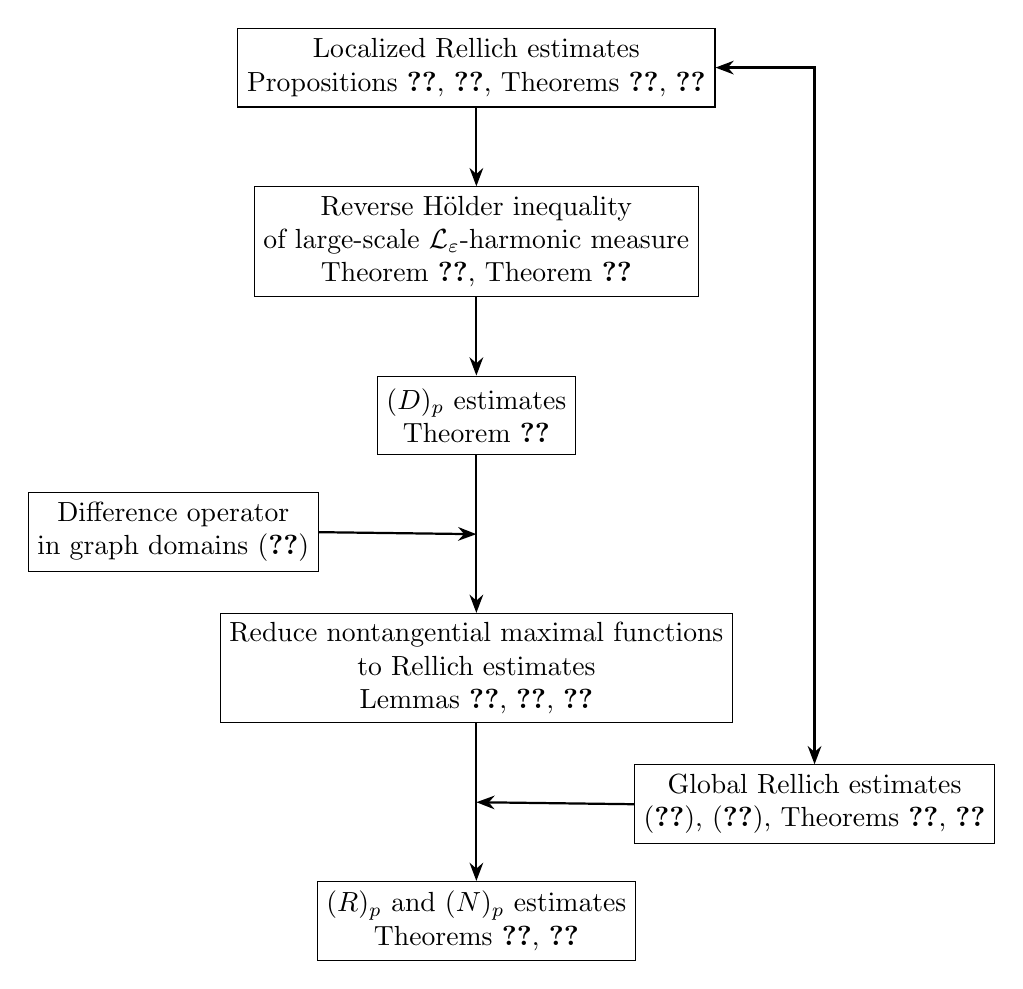
\begin{tikzpicture}[node distance=1.5cm, every node/.style={draw, rectangle, minimum width=2cm, minimum height=1cm, align = center}, arrow/.style={->, >=Stealth, thick}]

    % main flow nodes
    %\node (step0) {$(R)_p$/$(N)_p$ estimates for homogenized operator \\ \cite{D79}, Propositin \ref{prop.L0.averageNT}};
    \node (step1) {Localized Rellich estimates \\ Propositions \ref{prop.localR2}, \ref{prop.localN2}, Theorems \ref{thm.LocalRellich.Rp}, \ref{thm.LocalRellich.Np}};
    \node[below=1cm of step1] (step2) {Reverse H\"{o}lder inequality \\ of large-scale $\cL_\e$-harmonic measure\\ Theorem \ref{thm.B2}, Theorem \ref{thm.C1reverse}};
    \node[below=1cm of step2] (step3) {$(D)_p$ estimates \\ Theorem \ref{thm.Dp}};
    \node[below=2cm of step3] (step4) {Reduce nontangential maximal functions \\ to Rellich estimates \\ Lemmas \ref{lem.NT.ptws}, \ref{lem.NeQe}, \ref{lem.C1Rp}};
    \node[below=2cm of step4] (step5) {$(R)_p$ and $(N)_p$ estimates \\ Theorems \ref{thm.Rp}, \ref{thm.Np}};

    % side nodes
    %\node[left=2cm of step0] (Homo) at ($(step0)!0.5!(step1)$) [yshift = 0pt] {Homogenization \\ \cite{Shen17}, Proposition \ref{prop.Dwe.Lp}}; 
    \node[left=2cm of step3] (Diff) at ($(step3)!0.5!(step4)$) [yshift = 3.5pt] {Difference operator \\ in graph domains \eqref{def.Qe}}; 
    \node[right=2cm of step3] (GloRell) at ($(step4)!0.5!(step5)$) [yshift=-3.5pt] {Global Rellich estimates\\ \eqref{eq.LSRellich-D}, \eqref{eq.LSRellich-N}, Theorems \ref{thm.C1Rellich.Rp}, \ref{thm.C1Rellich.Np}};
    % connect all nodes
    %\draw[arrow] (step0) -- coordinate[midway] (midpoint0) (step1);
    \draw[arrow] (step1) -- (step2);
    \draw[arrow] (step2) -- (step3);
    \draw[arrow] (step3) -- coordinate[midway] (midpoint1) (step4);
    \draw[arrow] (step4) -- coordinate[midway] (midpoint2) (step5);
    %\draw[arrow] (Homo) -- (midpoint0);
    \draw[arrow] (Diff.east) --  (midpoint1);
    \draw[arrow] (GloRell.west) --  (midpoint2);
    \draw[<->,>=Stealth, thick] (GloRell.north) --  ++(0,0.1) |- (step1.east);
\end{tikzpicture}
    \caption{The flowchart of proofs}
    \label{fig.proofflow}
\end{figure}


%\begin{remark}
 %   The proofs of this paper may also go through in more general settings, provided two ingredients. For the large-scale estimates of Dirichlet problem, we only need the large-scale Rellich and $W^{1,p}$ estimates (in $C^1$ domains) down to $\e^\alpha$-scale for some $\alpha \in (0,1]$. Therefore, these estimates are available in various setting as long as a quantitative homogenization theory can be established, such as almost periodic operators \cite{SZ18,Z17}. For the regularity and Neumann problem, we additionally need the existence of the difference operator $\Q_\e$, for which the periodicity of $A$ plays a crucial role.
    %This condition can be guaranteed if $A$ is invariant in many directions. A typical example is that $A$ is quasiperiodic in the sense that $A(X) = B(MX)$ for some periodic $B$ in $\R^m$ and $M$ is a $m\times d$ matrix.  Since $B$ is periodic, the required condition is satisfied if $\{ X \in \mathbb{S}^{d-1}: MX \in \R\Z^m  \}$ is dense in $\mathbb{S}^{d-1}$. Particulary, if $m\le d$ and $M: \R^d \to \R^m$ is surjective, then the required condition is satisfied.
%\end{remark}

% \jz{Question: If $\Omega$ is $C^1$ or convex, can we show the optimal range of $p \in (1,\infty)$?}

\subsection{Notations}

We list below some notations that are frequently used throughout this paper.

\begin{itemize}
    \item We use the capital letters $X, Y, Z, \cdots$ to denote the interior points contained in the domain $\Omega \subset \R^d$, and $P, Q, \cdots$ to denote the boundary points on $\partial \Omega$.

    \item $\delta(X) = \dist(X, \partial \Omega): = \inf\{ |X-Q|: Q\in \partial \Omega \}$.

    %\item $\{ \omega^X_\e: X\in \Omega \}$ denote the family of $\cL_\e$-harmonic measure for the operator $\cL_\e$ in $\Omega$. Denote by $G_\e(X,Y)$ the Green's function of $\cL_\e$ in $\Omega$.

    \item $\sigma$ denotes the surface measure of $\partial \Omega$. For a Borel subset $E\subset \partial \Omega$, we also write $|E| = \sigma(E).$ 

    \item We use $\fint_E = \frac{1}{|E|} \int_E$ to represent the average integral over a set $E$. Here $|E|$ denotes either the volume of $E$ if it is a subset of $\R^d$, or the surface measure of $E$ if it is a subset of $\partial \Omega$.
    
    \item We use $B_r(X)$ or $B(X,r)$ to denote the Euclidean balls in $\R^d$ centered at $X$ with radius $r$. We use $\Delta_r(P) = \partial \Omega \cap B_r(P)$ for some $P\in \partial \Omega$ to denote the surface balls on $\partial \Omega$. Define $D_r(P) = \Omega \cap B_r(P)$ for $P\in \partial \Omega$.

    \item $\Omega_r = \{X \in \Omega: \dist(X,\partial \Omega) < r \}$ denotes the boundary layer of $\Omega$ with thickness $r$. Define $\Omega^r = \Omega \setminus \overline{\Omega_r}$.

    \item Let $\Omega$ be a bounded Lipschitz domain. For $Q\in \partial \Omega$, the nontangential region at $Q$ is defined by
    \begin{equation}
        \Gamma(Q) = \{ X\in \Omega: |X-Q| < \beta \dist(X,\partial \Omega)  \},
    \end{equation}
    where $\beta>1$ is a large fixed constant depending on the Lipschitz character of $\Omega$. A different version of nontangential cone will be defined in Lipschitz graph domains; see \eqref{def.Gamma.graph}.

    \item We will use various nontangential maximal functions on $ \partial \Omega$.
    Let $F \in C^0(\Omega)$. The classical nontangential maximal function $N(F)$ is defined by \eqref{NM}.
    %\begin{equation}
     %   N(u)(Q) = \sup \{|u(X)|: X\in \Gamma(Q) \}.
    %\end{equation}
    In this paper, we define the large-scale (or precisely $\e$-scale) nontangential maximal function $N_\e (F)$ by \eqref{def.N_e}.
     %\begin{equation}
      %  N_\e(u)(Q) = \sup \{|u(X)|: X\in \Gamma(Q) \setminus %\Omega_{10\e} \}.
    % \end{equation}
    % We define the truncated nontangential maximal function by
    % \begin{equation}
    %     N^r(u)(Q) = \sup \{|u(X)|: X\in \Gamma(Q) \cap \Omega_r \}.
    % \end{equation}
    %Similarly, for $r>10\e$, the large-scale and truncated nontangential maximal function is denoted by $N^r_\e(u)(Q)$.
    
    \item Let $F \in L^2_{\rm loc}(\Omega)$ be either a scalar or a vector-valued function. The modified nontangential maximal function $\widetilde{N}(F)$ is given by \eqref{MNM}.
    % \begin{equation}
    %\widetilde{N}(F)(Q) = \sup \bigg\{ \bigg(\fint_{B(X, \delta(X)/2) }|F(Y)|^2 dY \bigg)^{1/2}: X\in \Gamma(Q) \bigg\}.
    %\end{equation} 
    Define the large-scale modified nontangential maximal function $\widetilde{N}_\e(F)$ by \eqref{def.tN_e}. 
    Note that  $\widetilde{N}(F)(Q) = \lim_{\e \to 0} \widetilde{N}_\e(F)(Q)$.
    For $r> 10\e$, define the truncated large-scale nontangential maximal function by $\widetilde{N}_\e^r(F)(Q)$; see \eqref{def.tNe.truncated}.
    % \begin{equation}
    % \widetilde{N}_\e^r(F)(Q) = \sup \bigg\{ \bigg(\fint_{B(X, \delta(X)/2) }|F(Y)|^2 dY \bigg)^{1/2}: X\in \Gamma(Q) \cap \Omega^r \setminus \Omega_{10\e} \bigg\}.
    % \end{equation}
    A variant of the large-scale maximal function in a graph domain can be found in \eqref{def.hatN}.
    % \begin{equation}
    % \widehat{N}_\e(F)(Q) = \widetilde{N}_\e(F)(Q) + \bigg( \fint_{D_{100\e}(Q)} |F|^2 \bigg)^{1/2}.
    % \end{equation}

    \item The conormal derivative of $u_\e$ is denoted by $\frac{\partial u_\e}{\partial \nu_\e} = n\cdot A^\e \nabla u_\e$, where $n$ is the outer unit normal vector on $\partial \Omega$.

    \item Given $f \in C^1(\partial \Omega)$, the tangential derivative (gradient) of $f$ on $\partial \Omega$ is given by $\nabla_{\tan } f = (I - n\otimes n) \nabla f$.

    % \item Denote by $\mathcal{M}_{\partial \Omega}$ the Hardy-Littlewood maximal function on $\partial \Omega$, namely,
    % \begin{equation}\label{def.HL.maximal}
    %     \mathcal{M}_{\partial \Omega} f(Q) = \sup \bigg\{ \fint_{\Delta_r(Q)} |f| d\sigma: 0<r< \diam(\Omega) \bigg\}.
    % \end{equation}

    \item For $u \in L^2(\Omega)$, define the ($\e$-scale) average operator $M_\e$ in $\Omega$ by
    \begin{equation}
        M_\e(u)(X) = \bigg( \fint_{B_\e(X) \cap \Omega} |u|^2 \bigg)^{1/2}.
    \end{equation}
    Clearly, $M_\e(u)(Q)$ can also be defined for $Q \in \partial \Omega$. Similarly, we define the boundary average operator by
    \begin{equation}
        M_\e^{\partial}(f)(Q) = \bigg( \fint_{\Delta_\e(Q)} |f|^2 d\sigma \bigg)^{1/2}.
    \end{equation}
    This definition will be modified if $\Omega$ is a graph domain; see \eqref{def.bdryMt.inIr}.

    \item Let $\psi \in C_0^\infty(\R^d)$ and ${\rm supp}(\psi) \subset B_{1/2}(0)$. Assume $\psi \ge 0$ and $\int \psi = 1$. Let $\psi_\e(X) = \e^{-d} \psi(X/\e)$. Define the smoothing operator $K_\e$ by
    \begin{equation}\label{def.Ke}
        K_\e f(X) = \psi_\e * f(X).
    \end{equation}

    % \item In many proofs, we also relies on the estimates in graph domains. In this setting, we assume $\Omega$ is a Lipschitz domain given by $\Omega = \{ X = (x',x_d): x_d > \phi(x') \}$ where $\phi:\R^{d-1} \to \R$ is a Lipschitz function. We use $x',y',z' \in \R^{d-1}$ to represent the first $d-1$ components of $X,Y,Z \in \R^d$ and $x_d, y_d, z_d$ to represent last component. For $Q = (x',\phi(x')) \in \partial \Omega$, all kinds of nontangential maximal functions can be defined analogously as in bounded Lipschitz domains. Define the nontangential cone with vertex at $Q$ as
    % \begin{equation}\label{def.Gamma.graph}
    % \Gamma(Q) = \{Y = (y', y_d) \in \Omega: |x'-y'| < (\tan \beta) (y_d - \phi(x')) \}
    % \end{equation}
    % for some small $\beta>0$ depending on the Lipschitz constant of $\phi$. This is an infinite cone with opening angle $2\beta$, which is a harmless modification of the original nontangential maximal function in a bounded domain.


    % Define the surface balls by
    % \begin{equation}
    %     I_r(Q) = I_r(x',\phi(x')) = \{ (y',\phi(y')): |y'-x'| < r \}.
    % \end{equation}
    % Define the boundary cylinders by
    % \begin{equation}
    % \begin{aligned}
    %     T_r(Q) & = T_r(x',\phi(x')) \\
    %     & = \{(y',y_d): |y'-x'| < r, \phi(y') < y_d < \phi(y') + r \}.
    % \end{aligned}
    % \end{equation}
    % Observe that $T_r$ is always a bounded Lipschitz domain.

    

    \item For nonnegative quantities $a$ and $b$, we write $a\lesssim b$ if there exists some implicit constant $C$ independent of $a$ and $b$ such that $a\leq C b$. We write $a \gtrsim b$ if $b \lesssim a$. We write $a \simeq b$ if $a \lesssim b \lesssim a$. All the implicit constants in this paper depend at most on $d, \Lambda$, the exponent $p$ and the geometric characters of $\Omega$. In particular, they will never depend on the parameter $\e$.
    \end{itemize}

\textbf{Organization.} In Section \ref{sec.Dp}, we introduce the large-scale $\cL_\e$-harmonic measure and prove Theorem \ref{thm.Dp} in Lipschitz domains with $2-\delta<p\le \infty$. In Section \ref{sec.RpNp}, we prove Theorem \ref{thm.Rp}-\ref{thm.Np} in the case of Lipschitz domains for $1<p<2+\delta$. In Section \ref{sec.C1}, we prove Theorem \ref{thm.Dp}-\ref{thm.Np} in the case of bounded $C^1$ domains for the full range of $p\in (1,\infty)$. In Section \ref{sec.full-scale}, we prove Corollary \ref{coro.fullscale}. Some auxiliary analysis tools are stated or proved in appendices.

\textbf{Acknowledgments.} J. Zhuge is partially supported by NNSF of China (No. 12288201, 12494541, 12471115).


\section{Large-scale $\cL_\e$-harmonic measure and Dirichlet problem} \label{sec.Dp}

\subsection{$\cL_\e$-harmonic measure}

The $\cL_\e$-harmonic measure and Green function can be defined for the elliptic operator $\cL_\e = -\nabla\cdot (A^\e\nabla)$ in a bounded domain, as long as $A^\e$ is bounded measurable and satisfies the uniform ellipticity condition. In particular, the periodic structure or regularity on $A^\e$ is not needed.
Let $\{ \omega^X_\e \}_{X\in \Omega}$ denote the family of $\cL_\e$-harmonic measures for the operator $\cL_\e$ in $\Omega$. This means that if $f\in C(\partial \Omega)$, the classical solution of \eqref{Dp} can be expressed as
\begin{equation}\label{eq.hm}
    u_\e(X) = \int_{\partial \Omega} f d \omega^X_\e.
\end{equation}
Let $G_\e(X,Y)$ be the Green function of $\cL_\e$ in $\Omega$, i.e., for each $Y\in \Omega$, $\cL_\e(G_\e(\cdot,Y)) = \delta_Y(\cdot)$ in the sense of distributions and $G_\e(\cdot, Y) = 0$ on $\partial \Omega$. Moreover, $G_\e(X,Y) = G_\e^*(Y,X)$, where $G_\e^*$ is the Green function for the adjoint operator $\cL_\e^* = -\nabla\cdot (A^*(Y/\e) \nabla)$. In other words, $\cL_\e^*(G_\e(X,\cdot)) = \delta_X(\cdot)$ for each $X\in \Omega$.

We recall some basics of the $\cL_\e$-harmonic measure and Green function, which hold for any bounded measurable coefficients; see \cite{K94} for a collection of these materials. 
Let $\Delta_r(Q) = \partial \Omega \cap B_r(Q)$. Let $A_r(Q)$ be a point in $\Gamma(Q)$ such that $|A_r(Q) - Q| \simeq r$.
\begin{proposition}\label{prop.hmBasics}
    Let $\Omega$ be a bounded Lipschitz domain and $Q\in \partial \Omega$.
    \begin{enumerate}[label=(\roman*)]
        \item \label{item.doubling}
        $\omega^X_\e$ is doubling, i.e., for $X\in \Omega \setminus B_{4r}(Q)$,
        \begin{equation}
            \omega^X_\e(\Delta_{2r}(Q)) \lesssim \omega^X_\e(\Delta_{r}(Q)).
        \end{equation}
        \item \label{item.w=1} It holds
        \begin{equation}
            \omega_\e^{A_r(Q)}(\Delta_{r}(Q)) \simeq 1.
        \end{equation}
        
        \item  \label{item.w=G}  
        For $X\in \Omega \setminus B_{2r}(Q)$, 
    \begin{equation}\label{est.w=G}
        \omega_\e^X(\Delta_r(Q)) \simeq r^{d-2} G_\e(X, A_r(Q)).
    \end{equation}
        \item \label{item.G-L2}
        For $X\in \Omega \setminus B_{2r}(Q)$,
    \begin{equation}
        G_\e(X, A_r(Q)) \simeq \bigg( \fint_{\Omega \cap B_r(Q)} |G_\e(X,Y)|^2 dY\bigg)^{1/2}.
    \end{equation}

    \item \label{item.G.Holder}
    There exists $\alpha \in (0,1)$ such that for $X,Y\in \Omega$ and $\delta(X) < \frac12 |X-Y|$, 
    \begin{equation}
        G_\e(X,Y) \lesssim \frac{\delta(X)^\alpha}{|X-Y|^{d-2+\alpha}}.
    \end{equation}
    \end{enumerate}
\end{proposition}

% \red{The following prop can be stated for general solutions as a localized $L^2$ Rellich estimate}
% \begin{proposition}
%     Suppose $A$ is 1-periodic. Then we have the localized Rellich estimate for the Green function, i.e., for $r \ge \e, Q\in \partial \Omega$ and $X \in \Omega\setminus B_{4r}(Q)$,
%     \begin{equation}
%         \frac{1}{\e} \int_{D_r(Q) \cap \Omega_\e} |\nabla_Y G_\e(X,Y)|^2 dY \lesssim \frac{1}{r} \int_{D_{2r}(Q)}  |\nabla_Y G_\e(X,Y)|^2 dY.
%     \end{equation}
% \end{proposition}

\subsection{Localization}
\label{subsec.localization}
Though our main theorems are proved for bounded Lipschitz domains, it is standard to apply a localization argument to reduce the local boundary estimates to Lipschitz graph domains to avoid some technical issues. For example, for a bounded Lipschitz domain $\Omega$, $D_r(P) = \Omega\cap B_r(P)$ may not be a Lipschitz domain or even be disconnected. Here, we will briefly describe the localization argument.

Let $\Omega$ be a bounded Lipschitz domain. If we want to estimate $\widetilde{N}_\e(\nabla u)$, it suffices to estimate the truncated nontangential maximal function $\widetilde{N}_\e^R(\nabla u)$. This is due to the following observation
\begin{equation}\label{est.ReduceToLayer}
    \widetilde{N}_\e(u)(Q) \le \widetilde{N}_\e^{R}(u)(Q) + C_R \| \nabla u \|_{L^2(\Omega\setminus \Omega_{R/2})}.
\end{equation}
If we choose $R \simeq r_0 \gg \e$, where $r_0$ is a constant depending only on ${\rm diam}(\Omega)$ and the Lipschitz character of $\Omega$, then the second term on the right-hand side of \eqref{est.ReduceToLayer} can be easily controlled by the energy estimate. 
%It suffices to estimate the truncated nontangential maximal function $\widetilde{N}_\e^{r_0}(u)(Q)$, which relies only on $u$ restricted in $\Omega_{2r_0}$.
Consequently, we may concentrate on the estimates on the boundary layer $\Omega_{2r_0}$. Next, we cover $\Omega_{2r_0}$ by a finite number of balls $B(P_i,10r_0)$ centered at $P_i \in \partial \Omega$ with finite overlaps. This reduces the estimates to each $ D_{10r_0}(P_i) = B(P_i, 10r_0) \cap \Omega$. By a translation and a rotation, we can assume
\begin{equation}\label{eq.graphdomain}
    B(P_i, 10r_0) \cap \Omega = B(0,10r_0) \cap \left\{ X = (x',x_d): x_d > \phi(x') \right\},
\end{equation}
where $\phi:\R^{d-1} \to \R$ is a Lipschitz function, representing the local graph of $\partial \Omega$. We will use $x',y',z' \in \R^{d-1}$ to represent the first $d-1$ components of $X,Y,Z \in \R^d$ and $x_d, y_d, z_d$  the last components.

%\jz{Is it more convenient to use $(x,t)$ instead of $(x',x_d)$?}

With the above localization and reduction, we only need to consider the boundary value problems in the Lipschitz  graph domain $\Omega = \{ X = (x', x_d): x_d > \phi(x') \}$, whose boundary is given by $\partial \Omega = \{ X = (x',\phi(x')) \}$, where $\phi$ is a Lipschitz function. 
%Let $u_\e$ be a weak solution of $\cL_\e (u_\e) = 0$ in $\Omega$. 
Without loss of generality, assume $O = (0',0) \in \partial \Omega$, where $0'$ denotes the origin in $\R^{d-1}$.
%Because of the above localization, we will focus on the local estimate in a neighborhood of $(0',\phi(0')) \in \partial \Omega$, where $0'$ is the origin in $\R^{d-1}$.
%Above the graph domain, it is convenient define $B(x', r)$ as the ball in $\R^{d-1}$ centered at $x' \in \R^{d-1}$. 
% Consider
% \begin{equation}
%     D_t = \{ X = (x',x_d): |x'|< t, \phi(x') < x_d < C_0 t \},
% \end{equation}
% where $C_0$ is a constant depending on the Lipschitz constant of $\phi$. 
Given $Q = (x',\phi(x')) \in \partial \Omega$, let 
\begin{equation}\label{I-r}
I_r(Q) = \left\{ P = (y',\phi(y')): |y'-x'|<r \right\}
\end{equation}
and 
\begin{equation}\label{T-r}
T_r(Q) = \left\{ Y = (y',y_d): |y'-x'|<r, \phi(y') < y_d < \phi(x') + M r \right\},
\end{equation}
where $M=100d(1+ \| \nabla \phi \|_\infty).$
These are analogs of $\Delta_r(Q)$ and $D_r(Q)$. Note that $T_r(Q)$ is always a Lipschitz domain and $I_r(Q)$ is the bottom boundary of $T_r(Q)$. The crucial fact is that the estimates in $I_r(Q)$ or $T_r(Q)$ are interchangeable with those in $\Delta_r(Q)$ and $D_r(Q)$ due to the following simple comparisons: 
\begin{equation}\label{eq.Tr=Dr}
    I_{cr}(Q) \subset \Delta_r(Q) \subset I_r(Q) \quad \text{and} \quad T_{cr}(Q) \subset D_r(Q) \subset T_{Cr}(Q),
\end{equation}
for some constants $0<c<1<C$. Oftentimes, we will simply write $I_r$ and $T_r$ if $Q = O \in \partial \Omega$, where $O$ is the origin.

    \begin{figure}[htbp]
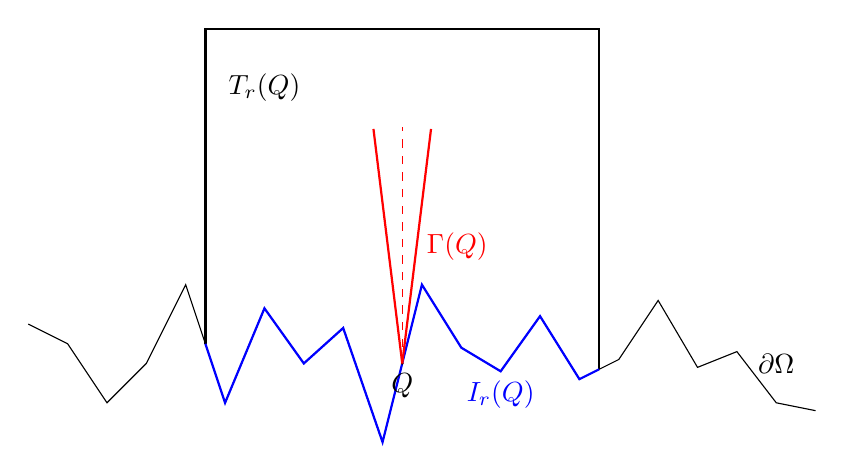
\begin{tikzpicture}[scale = 0.5]
    % 
    \draw (-1, 1) -- (0,0.5) -- (1,-1) -- (2,0) -- (3,2) -- (4,-1) -- (5,1.4) -- (6, 0) -- (7,0.9) -- (8,-2) -- (9,2) -- (10, 0.4) -- (11, -0.2) -- (12, 1.2) -- (13, -0.4) -- (14, 0.1) -- (15, 1.6) -- (16, -0.1) -- (17, 0.3) -- (18, -1) -- (19, -1.2);

\draw[thick] (3.5, 0.5) -- (3.5, 8.5) -- (13.5, 8.5) -- (13.5, -0.15);

     %\draw[thick] (3.5, 0.5) -- (3.5, 9.5) -- (4,8) -- (5,10.4) -- (6, 9) -- (7,9.9) -- (8,8) -- (9,11) -- (10, 9.4) -- (11, 8.8) -- (12, 10.2) -- (13, 8.6) -- (13.5, 8.85) -- (13.5, -0.15);

    \draw[blue, thick] (3.5, 0.5) -- (4,-1) -- (5,1.4) -- (6, 0) -- (7,0.9) -- (8,-2) -- (9,2) -- (10, 0.4) -- (11, -0.2) -- (12, 1.2) -- (13, -0.4) -- (13.5, -0.15);

    \node at (18,0) {$\partial \Omega$};
    \node[blue] at (11,-0.8) {$I_r(Q)$};
    \node at (5,7) {$T_r(Q)$};

    \coordinate (Q) at (8.5,0);
    \fill (Q) circle (1pt) node[below] {$Q$};

    \draw[red, thick] (Q) -- ++(83:6) node[midway, right] {$\Gamma(Q)$};
    \draw[red, thick] (Q) -- ++(97:6);

    \draw[dashed, red] (Q) -- ++(90:6);

    %\draw (3.5, 0.5) -- (3.5, 9) -- (13.5, 9) -- (13.5, -0.15);
    

    %\foreach \point in {(0,0), (1,2), (3,-1), (5,1), (7,0)} {\fill \point circle (2pt);}
\end{tikzpicture}
\caption{A graph domain}
\label{fig.graphdomain}
\end{figure}

Note that although $\Omega$ is an unbounded graph domain, we can still define $\delta(X)$ as the distance from $X\in \Omega$ to the boundary $\partial \Omega$, and $\Omega_r = \{ X\in \Omega: \delta(X) < r \}$. For each $Q = (x',\phi(x')) \in \partial \Omega$, we redefine the nontangential cone on $Q$ by
\begin{equation}\label{def.Gamma.graph}
    \Gamma(Q) = \left\{Y = (y', y_d) \in \Omega: |x'-y'| < (\tan \beta) (y_d - \phi(x')) \right\}
\end{equation}
for some $\beta \in (0,\pi/2)$ (representing the half-aperture of the cone), which is a harmless modification of the original nontangential maximal function in a bounded domain. By this, all kinds of nontangential maximal functions can be defined analogously as in bounded Lipschitz domains.
% Let
% \begin{equation}
%     \Omega_{t} = \{ (x',x_d) \in \Omega: \phi(x') < x_d < \phi(x') + t \}.
% \end{equation}
For example, we redefine the truncated large-scale nontangential maximal function by
\begin{equation}\label{def.tNe.truncated}
    \widetilde{N}_\e^r(F)(Q) = \sup\bigg\{ \bigg(\fint_{B(Y,\delta(Y)/2)} |F|^2 \bigg)^{1/2}: Y\in \Gamma(Q) \cap (\Omega_{r}\setminus \Omega_{10\e}) \bigg\}.
\end{equation}

Finally, we will see how the operator $\cL_\e$ changes in the above localization. If $A^\e(X) = A(X/\e)$ is $\e$-periodic (i.e., under the assumption \eqref{periodicity}), then after a rotation it is still $\e$-periodic with respect to a rotated lattice. Here, we will introduce the idea in \cite{KS11} that can handle more general cases for which $A^\e$ only needs to be periodic in the $x_d$-direction (and has no structure assumption in the remaining $d-1$ directions). Actually, if $A$ satisfies \eqref{periodicity}, we can always choose a rational rotation in the above reduction to \eqref{eq.graphdomain} such that $A^\e(X)$ is still $\ell \e$-periodic in $x_d$-direction for some integer $\ell \ge 1$ (the size of $\ell$ depends on the Lipschitz character of $\partial \Omega$), i.e., $A^\e(x',x_d) = A^\e(x', x_d + z\ell \e)$ for all $z\in \Z$. Without loss of generality, we assume $\ell = 1$, which yields
\begin{equation}\label{eq.periodicInxd}
    A^\e(x',x_d) = A^\e(x', x_d + \e z ) \qquad \text{for any } z\in \Z.
\end{equation}
Indeed, the results in this section are available whenever $A^\e$ satisfies \eqref{eq.periodicInxd} in each localized graph domain, which is a  weaker assumption than \eqref{periodicity}.
%Here for convenience, we omit the superscript $r_0$ for the truncated nontangential maximal function.

\subsection{$L^2$ Rellich estimates}
\label{subsec.L2Rel}
There are two different approaches to achieve the large-scale $L^2$ Rellich estimates. The first one was introduced in \cite{KS11} using the difference operator under the assumption \eqref{eq.periodicInxd}, and the second was introduced in \cite{Shen17} based on the convergence rates in homogenization theory. These two approaches have their own advantages and disadvantages, though they are both applicable to periodic (in all directions) coefficients. The approach in \cite{KS11} relies on the strict periodicity in the $x_d$-direction (i.e., \eqref{eq.periodicInxd}); while the approach in \cite{Shen17} also applies to non-periodic coefficients, but needs the structure assumption on the coefficients in all directions so that the quantitative homogenization applies.
We also point out that the approach in \cite{KS11} requires $A$ to be symmetric, while the approach in \cite{Shen17} only requires symmetry for the Neumann condition. For simplicity, we will always assume that $A$ is symmetric in this paper.

In order to be consistent with the class of operators for regularity and Neumann problems, we recall the large-scale $L^2$ Rellich estimates in \cite{KS11} based on the assumption \eqref{eq.periodicInxd}.

\begin{proposition}[{\cite[Lemma 3.4]{KS11}}] \label{prop.localR2}
    Let $\e < r$ and $A^\e$ satisfy \eqref{ellipticity} and \eqref{eq.periodicInxd}. Let $u_\e$ be a solution of
        \begin{equation}\label{eq.Rp.T3r}
    \left\{
    \begin{aligned}
        & -\nabla\cdot A^\e \nabla u_\e = 0 \quad \text{in } T_{3r}, \\
        & u_\e = f  \quad \text{on } I_{3r}.
    \end{aligned}
    \right.
    \end{equation}
    Then for any $\e < t< r$,
    \begin{equation}\label{est.L2Rellich-1}
        \frac{1}{t} \int_{T_r \cap \Omega_t} |\nabla u_\e|^2 \lesssim \int_{I_{3r}} |\nabla_{\tan} f|^2  + \frac{1}{r} \int_{T_{3r}} |\nabla u_\e|^2.
    \end{equation}
\end{proposition}

\begin{proposition}[{\cite[Lemma 3.2]{KS11} }] \label{prop.localN2}
    Let $\e < r$ and $A^\e$ satisfy \eqref{ellipticity} and \eqref{eq.periodicInxd}. Let $u_\e$ be a solution of
        \begin{equation}\label{eq.Np.T3r}
    \left\{
    \begin{aligned}
        & -\nabla\cdot A^\e \nabla u_\e = 0 \quad \text{in } T_{3r}, \\
        & \frac{\partial u_\e}{\partial \nu_\e} = g \quad \text{on } I_{3r}.
    \end{aligned}
    \right.
    \end{equation}
    Then for any $\e < t< r$,
    \begin{equation}\label{est.L2Rellich-2}
        \frac{1}{t} \int_{T_r \cap \Omega_t} |\nabla u_\e|^2 \lesssim \int_{I_{3r}} |g|^2  + \frac{1}{r} \int_{T_{3r}} |\nabla u_\e|^2.
    \end{equation}
\end{proposition}

\begin{remark}
 The above propositions are not stated in the same form as \cite[Lemmas 3.2, 3.4]{KS11}. In this remark, we clarify that they are actually equivalent. First, the above propositions are stated in a scaled version with period $\e$, which definitely is equivalent to the original version in \cite[Lemmas 3.2, 3.4]{KS11}  with period 1. Second,
    \cite[Lemma 3.2, 3.4]{KS11} were stated for the flat boundary $\{ x_d = 0 \}$, while the above propositions are stated over Lipschitz boundaries $\{x_d = \phi(x') \}$. However, by a change of variables, $(x', x_d) \to (y',y_d) = (x', x_d - \phi(x'))$, we can flatten the boundary without changing the condition \eqref{eq.periodicInxd}. Third, the estimates \eqref{est.L2Rellich-1} and \eqref{est.L2Rellich-2} hold for all $t \in (\e,r)$, instead of a fixed scale $t = \e$, because if $A_\e$ is $\e$-periodic in $x_d$, then it is $m\e$-periodic for any $m\in \N$ and the desired estimates are valid for any $t \simeq [t/\e]\e$.
\end{remark}

The above propositions can be converted to $D_r$ in a bounded Lipschitz domain for the operator $\cL_\e$ using \eqref{eq.Tr=Dr} and a covering argument. Consequently, they implies the global $L^2$ Rellich estimates \eqref{eq.LSRellich-D} and \eqref{eq.LSRellich-N}. In fact, by \eqref{est.L2Rellich-1}, we have
\begin{equation}
        \frac{1}{t} \int_{D_{cr_0}(P_i) \cap \Omega_t} |\nabla u_\e|^2 \lesssim \int_{\Delta_{r_0}(P_i)} |\nabla_{\tan} f|^2  + \frac{1}{r_0} \int_{D_{r_0}(P_i)} |\nabla u_\e|^2.
    \end{equation}
Choosing $P_i$'s such that $\Omega_{cr_0}$ is covered by the union of $D_{cr_0}(P_i)$ with finite overlaps, then we sum over $i$ for the above inequality and obtain
\begin{equation}\label{est.L2RR}
    \frac{1}{t}\int_{\Omega_t} |\nabla u_\e|^2 \lesssim \int_{\partial \Omega} |\nabla_{\tan} f|^2 + \frac{1}{r_0}\int_{\Omega} |\nabla u_\e|^2.
\end{equation}
Finally, the energy estimate yields $\| \nabla u_\e \|_{L^2(\Omega)} \lesssim \| f \|_{H^1(\partial \Omega)}$, which combined with \eqref{est.L2RR} leads to \eqref{eq.LSRellich-D}. The derivation of \eqref{eq.LSRellich-N} is completely similar.

For an application to the Dirichlet problem in the next subsection, we state the following local estimate in $D_r$, which follows readily from \eqref{eq.Rp.T3r}.

\begin{proposition}\label{prop.LSRellich}
    Let $\e \le r$. Let $u_\e$ be a weak solution of $\cL_\e(u_\e) = 0$ in $D_{2r}(Q) = \Omega \cap B_{2r}(Q)$ for some $Q \in \partial \Omega$, and $u_\e = 0$ on $\Delta_{2r}(Q)$. Then for any $t\in [\e,r]$, 
    \begin{equation}
        \frac{1}{t} \int_{D_r(Q) \cap \Omega_t} |\nabla u_\e|^2 \lesssim \frac{1}{r} \int_{D_{2r}(Q)} |\nabla u_\e|^2.
    \end{equation}
\end{proposition}

%We point out in advance that the $(D)_p$ estimate \eqref{est.Dp} in Theorem \ref{thm.Dp} relies only on the large-scale $L^2$ Rellich estimate in Proposition \ref{prop.LSRellich}. As mentioned at the beginning of Subsection \ref{subsec.L2Rel}, this estimate is available for larger classes of operators, not necessarily with periodic coefficients, by using different approaches.


\subsection{Large-scale $\cL_\e$-harmonic measure}
Define the large-scale $\cL_\e$-harmonic measure by
\begin{equation}\label{def.LSomega}
    \overline{\omega}^X_\e(Q) := \frac{\omega_\e^X(\Delta_\e(Q))}{\sigma(\Delta_\e(Q))}.
\end{equation}
For a Lipschitz domain $\Omega$, we have $\sigma(\Delta_\e(Q)) \simeq \e^{d-1}$.
By the doubling property of $\omega^X_\e$, we can show the doubling property of $\overline{\omega}^X_\e$.
\begin{lemma}\label{lem.doubling}
For any $0<r<r_0, \Delta_r = \Delta_r(P), X \in \Omega $ and $|X - P| > 5\max\{ r,\e \}$, we have
\begin{equation}\label{est.doubling}
    \int_{\Delta_{2r}} \overline{\omega}^X_\e(Q) d\sigma(Q) \lesssim \int_{\Delta_{r}} \overline{\omega}^X_\e(Q) d\sigma(Q).
\end{equation}
\end{lemma}
\begin{proof}
    First, consider $r<10\e$. In this case, by the doubling property of $\omega_\e^X$, for any $Q, Q' \in \Delta_{2\e}(P)$, we have $\omega_\e^X(\Delta_\e(Q)) \simeq  \omega_\e^X(\Delta_\e(Q'))$. 
    Here we have used the assumption $|X-P|>5\e$.
    This implies that $\overline{\omega}^X_\e(Q) \simeq \overline{\omega}^X_\e(Q') $ for any $Q, Q^\prime\in \Delta_{2r} \subset \Delta_{2\e}(P)$. Thus, \eqref{est.doubling} follows.

    Now consider the case $r\ge 10\e$. By Fubini's Theorem, we have
    \begin{equation}\label{est.doubling<}
        \begin{aligned}
            \int_{\Delta_{2r}} \overline{\omega}^X_\e(Q) d\sigma(Q) & = \int_{\Delta_{2r}} \int_{\Delta_{2r+\e}} \mathbbm{1}_{\{|Q'-Q|<\e\}} |\Delta_\e(Q')|^{-1} d\omega_\e^X(Q') d\sigma(Q) \\
            & \lesssim \int_{\Delta_{2r+\e}} \int_{\Delta_{2r}} \mathbbm{1}_{\{|Q'-Q|<\e\}} d\sigma(Q) \e^{1-d} d\omega_\e^X(Q') \\
            & \lesssim \int_{\Delta_{2r+\e}} d\omega_\e^X(Q') \\
            & \lesssim \omega_\e^X(\Delta_{2r+\e}) \lesssim \omega_\e^X(\Delta_{r-\e}),
        \end{aligned}
    \end{equation}
    where in the last line we have used the fact $2r+\e \le 3(r-\e)$ for $r\ge 10\e$ and the doubling property of $\omega_\e^X$ in Proposition \ref{prop.hmBasics} \ref{item.doubling}.

    On the other hand, using Fubini's Theorem again, we have
    \begin{equation}
    \begin{aligned}
        \int_{\Delta_{r}} \overline{\omega}^X_\e(Q) d\sigma(Q) & = \int_{\Delta_{r}} \int_{\Delta_{r+\e}} \mathbbm{1}_{\{|Q'-Q|<\e\}} |\Delta_\e(Q')|^{-1} d\omega_\e^X(Q') d\sigma(Q) \\
        & \gtrsim \int_{\Delta_{r+\e}} \int_{\Delta_{r}} \mathbbm{1}_{\{|Q'-Q|<\e\}} d\sigma(Q) \e^{1-d} d\omega_\e^X(Q').
    \end{aligned}
    \end{equation}
    Observe that for $Q'\in \Delta_{r-\e}$,
    \begin{equation}
        \int_{\Delta_{r}} \mathbbm{1}_{\{|Q'-Q|<\e\}} d\sigma(Q) = \sigma(\Delta_\e(Q')) \simeq \e^{d-1}.
    \end{equation}
    It follows that
    \begin{equation}\label{est.doubling>}
        \int_{\Delta_{r}} \overline{\omega}^X_\e(Q) d\sigma(Q) \gtrsim \int_{\Delta_{r-\e}} d\omega_\e^X(Q') = \omega_\e^X(\Delta_{r-\e}).
    \end{equation}
    Combining \eqref{est.doubling<} and \eqref{est.doubling>}, we get \eqref{est.doubling}.
\end{proof}

%This follows from Proposition \ref{prop.hmBasics} \ref{item.doubling} and the Fubini's theorem. \jz{Better give a detailed proof, meanwhile show how Fubini's theorem is applied.}

%Fix $x_0 \in \Omega$ to be a ``center'' of $\Omega$ such that $\dist(X_0, \partial \Omega) \simeq \text{diam}(\Omega)$. Let $\overline{\omega}_\e = \overline{\omega}^{X_0}_\e$.

\begin{theorem}\label{thm.B2}
    It holds $\overline{\omega}_\e^X \in B_2(d\sigma)$ uniformly in $\e$, in the sense that, any $r > 0, P\in \partial \Omega, X \in \Omega$ and $|X-P| > 5\max \{r, \e \}$,
    \begin{equation}\label{est.B2}
        \bigg( \fint_{\Delta_r(P)} \overline{\omega}_\e^X(Q)^2 d\sigma(Q) \bigg)^{1/2} \lesssim \fint_{\Delta_{r}(P)} \overline{\omega}_\e^X(Q) d\sigma(Q).
    \end{equation}
\end{theorem}
\begin{proof}
    The case $r<10\e$ follows by the same reasoning as Lemma \ref{lem.doubling}. It suffices to assume $r>10\e$. Let $\Delta_r = \Delta_r(P)$ and $B_r = B_r(P)$.

    By Proposition \ref{prop.hmBasics} \ref{item.w=G}, \ref{item.G-L2}  and \eqref{def.LSomega}, for each $Q\in \Delta_r$,
    \begin{equation}
        \overline{\omega}_\e^X(Q) \simeq \e^{-1} G(X, A_\e(Q)) \lesssim \bigg( \fint_{B_{2\e}(Q) \cap \Omega} |\nabla_Y G_\e(X, Y)|^2 dY \bigg)^{1/2},
    \end{equation}
    where we also used the Poincar\'{e} inequality. Thus, by Fubini's Theorem, Proposition \ref{prop.LSRellich}, Caccioppoli's inequality and Proposition \ref{prop.hmBasics} \ref{item.G-L2}, \ref{item.w=G}, in order, we have
    \begin{equation}
    \begin{aligned}
        \int_{\Delta_r} \overline{\omega}_\e^X(Q)^2 d\sigma(Q) & \lesssim \e^{-d} \int_{\Delta_r} \int_{B_{2\e(Q)} \cap \Omega} |\nabla_Y G_\e(X,Y)|^2 dY d\sigma \\
        & \lesssim \e^{-d} \int_{\Omega_{2\e} \cap B_{1.5r}} |\nabla G(X,Y)|^2 \int_{\Delta_r} \mathbbm{1}_{|Y-Q| < 2\e} d\sigma dY\\
        & \lesssim \e^{-1} \int_{\Omega_{2\e} \cap B_{1.5r}} |\nabla G_\e(X,Y)|^2 dY \\
        & \lesssim r^{-1} \int_{D_{3r}} |\nabla G_\e(X,Y)|^2 dY \\
        & \lesssim r^{-3} \int_{D_{4r}} |G_\e(X, Y)|^2 dY \\
        & \lesssim r^{d-3} |G_\e(X, A_r(P))|^2 \\
        & \simeq r^{1-d} \omega_\e^X(\Delta_r)^2.
    \end{aligned}
    \end{equation}
    Dividing both sides by $r^{d-1}$ and taking square root, we obtain
    \begin{equation}
        \bigg( \fint_{\Delta_r} \overline{\omega}_\e^X(Q)^2 d\sigma(Q) \bigg)^{1/2} \lesssim \frac{\omega_\e^X(\Delta_r)}{\sigma(\Delta_r)} \lesssim  \frac{\omega_\e^X(\Delta_{r/2})}{\sigma(\Delta_r)} \lesssim \fint_{\Delta_{r}} \overline{\omega}_\e^X(Q) d\sigma(Q),
    \end{equation}
    where we also used the doubling property of $\omega^X_\e$ in Proposition \ref{prop.hmBasics} \ref{item.doubling}, and Fubini's Theorem in the last inequality.
\end{proof}

The estimate \eqref{est.B2} is a reverse H\"{o}lder inequality valid over all small scales $r>0$. The well-known  self-improving property of the reverse H\"{o}lder inequality implies the following.
\begin{corollary}\label{coro.2+delta}
    There exists $\delta>0$, depending on $d$, $\Lambda$ and $\Omega$, such that $\overline{\omega}_\e^X \in B_{2+\delta}(d\sigma)$ in the sense that for any $r>0, P\in \partial \Omega, X\in \Omega$ and $|X - P| > 5\max \{r, \e\}$,
    \begin{equation}
        \bigg( \fint_{\Delta_r(P)} \overline{\omega}_\e^X(Q)^{2+\delta} d\sigma(Q) \bigg)^{1/(2+\delta)} \lesssim \fint_{\Delta_{r}(P)} \overline{\omega}_\e^X(Q) d\sigma(Q).
    \end{equation}
\end{corollary}

\subsection{Dirichlet problem}

In this subsection, we consider the Dirichlet problem \eqref{Dp} and prove Theorem \ref{thm.Dp} for Lipschitz domains. The following is the key theorem that explains how the large-scale $\cL_\e$-harmonic measure is involved.

\begin{theorem}\label{thm.Neve<f}
    Let $f\in C(\partial \Omega)$ and
    \begin{equation}\label{def.ve}
        v_\e(X) = \int_{\partial \Omega} f(Q) \overline{\omega}^X_\e(Q) d\sigma(Q).
    \end{equation}
    Then $v_\e$ is a solution of
    \begin{equation}\label{eq.ve=barf}
    \left\{
    \begin{aligned}
        & \cL_\e(v_\e) = 0 \quad \text{in } \Omega, \\
        & v_\e(Q) = \bar{f}(Q) := \int_{\Delta_\e(Q)} |\Delta_\e|^{-1} f d\sigma \quad \text{on } \partial \Omega,
    \end{aligned}
    \right.
\end{equation}
where $|\Delta_\e| = |\Delta_\e(P)| \simeq \e^{d-1}$.
    Moreover, for any $p\in (2-\delta, \infty)$,
    \begin{equation}\label{est.Neve}
        \| N_\e(v_\e) \|_{L^p(\partial \Omega)} \lesssim \| f \|_{L^p(\partial \Omega)}.
    \end{equation}
\end{theorem}

\begin{proof}
    By Fubini's Theorem,
    \begin{equation}
    \begin{aligned}
        v_\e(X) & = \int_{\partial \Omega} \int_{\partial \Omega} |\Delta_\e(Q)|^{-1} f(Q) 1_{\Delta_\e(Q)}(P) d\omega^X_\e(P) d\sigma(Q) \\ & = \int_{\partial \Omega} \int_{\partial \Omega} |\Delta_\e(Q)|^{-1} f(Q) 1_{\Delta_\e(P)}(Q) d\sigma(Q) d\omega_\e^X(P) \\
        & = \int_{\partial \Omega} \int_{\Delta_\e(P)} |\Delta_\e(Q)|^{-1} f(Q) d\sigma(Q) d\omega_\e^X(P)\\
        & = \int_{\partial \Omega} \bar{f} d\omega_\e^X.
    \end{aligned}
    \end{equation}
    This proves \eqref{eq.ve=barf}.

    Next, we prove \eqref{est.Neve}. Let $X\in \Gamma(Q)$ and $\dist(X,\partial \Omega) > 10\e$. Let $r_0 = c|X - Q|$ and $r_j = 2^j r_0$. Let $R_0 = \Delta_{r_0}(Q)$, $R_j = \Delta_{r_j}(Q) \setminus \Delta_{r_{j-1}}(Q)$ for $j = 1,2, \cdots, L$, where $L$ is the minimal integer such that $2^L r_0 \ge c\diam(\Omega)$,
    and $R_{L+1} = \partial\Omega \setminus \Delta_{r_L}$. Then
    \begin{equation}
        \partial \Omega = \bigcup_{j = 0}^{L+1} R_j.
    \end{equation}
    Observe that for every $j = 0,1,\cdots, L+1$, we have $\dist(X, R_j) \simeq 2^j r_0$. Thus, Corollary \ref{coro.2+delta} and a covering argument yields
    \begin{equation}
        \bigg( \fint_{R_j} \overline{\omega}_\e^X(Q)^{2+\delta} d\sigma(Q) \bigg)^{1/(2+\delta)} \lesssim \fint_{R_j} \overline{\omega}_\e^X(Q) d\sigma(Q).
    \end{equation}

    Now, we bound \eqref{def.ve} by
    \begin{equation}\label{est.BdryDecomp}
    \begin{aligned}
    |v_\e(X)| & \lesssim \sum_{j = 0}^{L+1} \int_{R_j} |f(P')| \overline{\omega}_\e^X(P') d\sigma(P')\\
    & \le \sum_{j = 0}^{L+1} \bigg(\int_{R_j} |f(P')|^{p'_0} d\sigma(P') \bigg)^{1/p'_0} \bigg( \int_{R_j} \overline{\omega}_\e^X(P')^{p_0} d\sigma(P') \bigg)^{1/p_0} \\
    & \lesssim \sum_{j = 0}^{L+1} \bigg(\int_{R_j} |f(P')|^{p'_0} d\sigma(P') \bigg)^{1/p'_0} \int_{R_j} \overline{\omega}_\e^X(P') d\sigma(P') |R_j|^{-1/p^\prime_0}, 
    %  \sum_{k = 0}^M \sum_{ c2^k|X-Q| \le r_j < c2^{k+1}|X-Q|} \bigg(\int_{\Delta_{r_j}(P_j)} |f(P')|^2 d\sigma(P') \bigg)^{1/2} \overline{\omega}_\e^X(P') d\sigma(P'),
    \end{aligned}
\end{equation}
where $p_0=2+\delta$.
By the definition of $\overline{\omega}_\e^X$ and Proposition \ref{prop.hmBasics} \ref{item.w=G} \ref{item.G.Holder},
\begin{equation}
    \int_{R_j} \overline{\omega}_\e^X(P') d\sigma(P') \lesssim \int_{R_j} d \omega_\e^X = \omega_\e^X(R_j) \simeq 2^{-j\alpha}.
\end{equation}
It follows from \eqref{est.BdryDecomp} that
\begin{equation}
\begin{aligned}
    |v_\e(X)| & \lesssim \sum_{j = 0}^{L+1} \bigg(\fint_{R_j} |f(P')|^{p'_0} d\sigma(P') \bigg)^{1/p'_0} 2^{-j \alpha} \\ 
    & \lesssim \big\{ \M_{\partial \Omega}(|f|^{p'_0})(Q) \big\}^{1/{p'_0}},
\end{aligned}
\end{equation}
where $\M_{\partial \Omega}(F)$ denotes the Hardy-Littlewood maximal function on $\partial \Omega$.

Taking supremum over all $X\in \Gamma(Q)$ with $\dist(X,\partial \Omega) > 10\e$, we arrive at
\begin{equation}
    N_\e(v_\e)(Q) \lesssim \big\{ \M_{\partial \Omega}(|f|^{p'_0})(Q)\big\}^{1/{p'_0}}.
\end{equation}
Now, for any $p> p'_0$, by the $L^q$ boundedness of Hardy-Littlewood maximal function for any $q>1$, we have
\begin{equation}
    \| N_\e(v_\e) \|_{L^p(\partial \Omega)} \lesssim \bigg( \int_{\partial \Omega} \big\{ \M_{\partial \Omega}(|f|^{p'_0})(Q)\big\}^{p/{p'_0}} d\sigma(Q) \bigg)^{1/p} \lesssim \| f \|_{L^p(\partial \Omega)}.
\end{equation}
Note that $p = \infty$ is trivial from the maximal principle.
This ends the proof.
\end{proof}

\begin{remark}
    The equations \eqref{def.ve} and \eqref{eq.ve=barf}  can be written as
\begin{equation}\label{eq.bar.dual}
    \int_{\partial \Omega} f(Q) \overline{\omega}^X_\e(Q) d\sigma(Q) = \int_{\partial \Omega} \bar{f}(Q) d\omega_\e^X(Q).
\end{equation}
\end{remark}

\begin{remark}\label{rmk.Bp-Dp'}
    The proof of Theorem \ref{thm.Neve<f} gives the following result. If $\overline{\omega}_\e^X \in B_p(d\sigma)$ for some $p>1$, namely, for $X\in \Omega\setminus B_{10r}(P)$,
    \begin{equation}
        \bigg( \fint_{\Delta_r(P)} \overline{\omega}_\e^X(Q)^p d\sigma(Q) \bigg)^{1/p} \lesssim \fint_{\Delta_r(P)} \overline{\omega}_\e^X(Q) d\sigma(Q),
    \end{equation}
    then $v_\e$ given by \eqref{def.ve} satisfies
    \begin{equation}
            \| N_\e(v_\e) \|_{L^{p'}(\partial \Omega)} \lesssim \| f \|_{L^{p'}(\partial \Omega)}.
    \end{equation}
    This large-scale estimate can be compared to the classical result for $\cL_\e$-harmonic functions; see e.g. \cite{D77,D79,FKP91}.
\end{remark}

% Let $f \in C(\partial \Omega)$. Define
% \begin{equation}
%     S_\e (f)(Q) = \sup \{ |f(P)|: P \in \Delta_\e(Q) \}.
% \end{equation}

% \begin{theorem}\label{thm.Dp+}
%     Let $u_\e$ be the solution of \eqref{Dp} with $f\in C(\partial \Omega)$. Then there exists some $\delta>0$ such that for $2-\delta < p\le \infty$,
%     \begin{equation}\label{est.Neue<Sef}
%         \| N_\e(u_\e) \|_{L^p(\partial \Omega)} \lesssim \| S_\e(f) \|_{L^p(\partial \Omega)}.
%     \end{equation}
% \end{theorem}

\begin{proof}[\textbf{Proof of Theorem \ref{thm.Dp}}]
We use the representation formula by $\cL_\e$-harmonic measure,
\begin{equation}
    u_\e(X) = \int_{\partial \Omega} f(P) d\omega_\e^X(P).
\end{equation}
Observe that by the definition of $S_\e(f)$, we have $|f(P)| \le S_\e(f)(Q)$ for any $Q\in \Delta_\e(P)$. Since $|\Delta_\e(P)| \simeq |\Delta_\e(Q)|$, we have
$|f(P)| \lesssim \overline{S_\e(f)}(P)$.
Consequently, in view of \eqref{eq.bar.dual},
\begin{equation}
    |u_\e(X)| \lesssim \int_{\partial \Omega} \overline{S_\e(f)} d\omega_\e^X = \int_{\partial \Omega} S_\e(f) \overline{\omega}_\e^X d\sigma.
\end{equation}
Then \eqref{est.Dp} follows from this and \eqref{est.Neve} in Theorem \ref{thm.Neve<f}.
\end{proof}

% For $X \in \Gamma(Q)$ and $\dist(X,\partial \Omega) \ge 2\e$,
% \begin{equation}
%     \begin{aligned}
%         |u_\e(X)| & \le \int_{\partial \Omega} |f(P)| d\omega_\e^X(P) \\
%         & \lesssim \int_{\partial \Omega} \e^{1-d}\int_{\partial \Omega} 1_{\Delta_\e(P)}(P') |f(P)| d\sigma(P') d\omega_\e^X(P) \\
%         & \lesssim \int_{\partial \Omega} \e^{1-d}\int_{\partial \Omega} 1_{\Delta_\e(P')}(P) |f(P)| d\omega_\e^X(P) d\sigma(P') \\
%         & \lesssim \int_{\partial \Omega} S_\e(f)(P') \frac{{\omega}_\e^X(\Delta_\e(P'))}{\sigma(\Delta_\e(P'))} d\sigma(P') \\
%         & \lesssim \int_{\partial \Omega} S_\e(f)(P') \overline{\omega}_\e^X(P') d\sigma(P').
%     \end{aligned}
% \end{equation}

% Decompose the boundary $\partial \Omega$ as 
% \begin{equation}
%     \partial \Omega =  \bigcup_{j} \Delta_{r_j}(P_j) \quad \text{and} \quad  \frac15|P_j-X| > r_j \simeq |P_j - X|.
% \end{equation}
% Moreover, these $\{ \Delta_{r_j}(P_j) \}$ has a finite number of overlaps. Note that these surface balls have a minimum radius $r_0 = c|X-Q|$ for some universal constant $c>0$. The number of elements in $\{ \Delta_{r_j}(P_j) \}$ satisfying $c2^k|X-Q| \le r_j < c2^{k+1}|X-Q|$ is a finite number depending only on $d$ and $\Omega$. The condition $X\in \Gamma(Q)$ implies $|P_j - Q| \lesssim |P_j - X| \lesssim r_j$.
% Then we can write
% \begin{equation}\label{est.BdryDecomp}
%     |u_\e(X)| \lesssim \sum_{k = 0}^L \sum_{ c2^k|X-Q| \le r_j < c2^{k+1}|X-Q|} \int_{\Delta_{r_j}(P_j)} |f(P')| \overline{\omega}_\e^X(P') d\sigma(P'),
%     %  \sum_{k = 0}^M \sum_{ c2^k|X-Q| \le r_j < c2^{k+1}|X-Q|} \bigg(\int_{\Delta_{r_j}(P_j)} |f(P')|^2 d\sigma(P') \bigg)^{1/2} \overline{\omega}_\e^X(P') d\sigma(P')
% \end{equation}
% where $L$ the minimum integer such that $c2^{L+1}|X-Q| \ge \text{diam}(\Omega)$.
% Now, for each $j$, applying the Cauchy-Schwarz inequality,
% \begin{equation}
% \begin{aligned}
%     & \int_{\Delta_{r_j}(P_j)} |f(P')| \overline{\omega}_\e^X(P') d\sigma(P') \\ 
%     & \le \bigg(\int_{\Delta_{r_j}(P_j)} |f(P')|^{p'_0} d\sigma(P') \bigg)^{1/p'_0} \bigg( \int_{\Delta_{r_j}(P_j)} \overline{\omega}_\e^X(P')^{p_0} d\sigma(P') \bigg)^{1/p_0} \\
%     & \le \bigg(\int_{\Delta_{r_j}(P_j)} |f(P')|^{p'_0} d\sigma(P') \bigg)^{1/p'_0} \int_{\Delta_{2r_j}(P_j)} \overline{\omega}_\e^X(P') d\sigma(P') |\Delta_{r_j}(P_j)|^{-1/p_0},
%     \end{aligned}
% \end{equation}
% where $p_0 = 2+\delta$ is taken from Corollary \ref{coro.2+delta}.
% By the definition of $\overline{\omega}_\e^X$
% \begin{equation}
%     \int_{\Delta_{2r_j}(P_j)} \overline{\omega}_\e^X(P') d\sigma(P') \lesssim \int_{\Delta_{3r_j}(P_j)} d \omega_\e^X = \omega_\e^X(\Delta_{3r_j}(P_j)) \simeq 1.
% \end{equation}
% Consequently,
% \begin{equation}
%     \int_{\Delta_{r_j}(P_j)} |f(P')| \overline{\omega}_\e^X(P') d\sigma(P') \lesssim \big\{ M(|f|^{p'_0})(Q) \big\}^{1/{p'_0}} r_j^{(d-1)(1/{p'_0} - 1/p_0)},
% \end{equation}
% where $M(F)$ is the Hardy-Littlewood maximal function on $\partial \Omega$.
% Since $p_0 = 2+\delta > 2$, then $\alpha:= (d-1)(1/{p'_0} - 1/p_0) > 0$, we have
% \begin{equation}
% \begin{aligned}
%     \sum_{ c2^k|X-Q| \le r_j < c2^{k+1}|X-Q|} & \int_{\Delta_{r_j}(P_j)} |f(P')| \overline{\omega}_\e^X(P') d\sigma(P') \\
%     & \lesssim \big\{ M(|f|^{p'_0})(Q) \big\}^{1/{p'_0}} (2^k |X-Q|)^{\alpha}
% \end{aligned}
% \end{equation}
% Inserting this into \eqref{est.BdryDecomp}, we obtain
% \begin{equation}
% \begin{aligned}
%     |u_\e(X)| & \lesssim \big\{ M(|f|^{p'_0})(Q) \big\}^{1/{p'_0}} \sum_{k = 0}^{L} (2^k |X-Q|)^{\alpha} \\
%     & \lesssim \big\{ M(|f|^{p'_0})(Q) \big\}^{1/{p'_0}} (2^L |X-Q|)^\alpha \\
%     & \lesssim \text{diam}(\Omega)^\alpha \big\{ M(|f|^{p'_0})(Q)\big\}^{1/{p'_0}}.
% \end{aligned}
% \end{equation}
% Taking supremum over all $X\in \Gamma(Q)$ with $\dist(X,\partial \Omega) > 2\e$, we arrive at
% \begin{equation}
%     N_\e(u_\e)(Q) \lesssim \big\{ M(|f|^{p'_0})(Q)\big\}^{1/{p'_0}}.
% \end{equation}
% Now, for any $p> p'_0 = 2-\delta$ for some $\delta>0$, by the $L^q$ boundedness of Hardy-Littlewood maximal function for any $q>1$, we have
% \begin{equation}
%     \| N_\e(u_\e) \|_{L^p(\partial \Omega)} \lesssim \bigg( \int_{\partial \Omega} \big\{ M(|f|^{p'_0})(Q)\big\}^{p/{p'_0}} d\sigma(Q) \bigg)^{1/p} \lesssim \| |f| \|_{L^p(\partial \Omega)}.
% \end{equation}
% Note that $p = \infty$ is trivial from the maximal principle.
% This ends the proof.

%\begin{proof}[\textbf{Proof of Theorem \ref{thm.Dp}}]

Note that if $\Omega$ is a Lipschitz domain and $\e$ is small enough (depending on $\Omega$), then $\Omega^\e= \Omega \setminus \overline{\Omega_\e}$ is also a Lipschitz domain.
 Applying Theorem \ref{thm.Dp} to the subdomain $\Omega^\e $, we obtain
\begin{equation}\label{est.N<S}
    \| N_\e(u_\e) \|_{L^p(\partial \Omega)} \lesssim \| S_\e(u_\e) \|_{L^p(\partial \Omega^\e)}.
\end{equation}
Here, we have also used an observation that the large-scale nontangential maximal function on $\partial \Omega$ can be bounded by that on $\partial \Omega^\e$ with slight modifications (enlarge $\beta$ in \eqref{def.NTcone} and replace $10\e$ by $8\e$ in \eqref{def.N_e}) on the definition for the latter.
We find a bi-Lipschitz map $\tau: \partial \Omega \mapsto \partial \Omega^\e$ such that $Q^\e = \tau(Q)$ satisfies $B_{2\e}(Q_\e) \subset B_{4\e}(Q)$.
Hence, by the interior $L^\infty$ estimate, we have for $P \in \partial \Omega^\e$
\begin{equation}
    S_\e(u_\e)(Q^\e) = \sup_{ \substack{P\in \partial \Omega^\e \\ |P-Q^\e|<\e }} |u_\e(P)|  \lesssim \fint_{B_{2\e}(Q^\e) \cap \Omega} |u_\e| \lesssim \fint_{B_{4\e}(Q) \cap \Omega} |u_\e| = M_{4\e}(u_\e)(Q).
\end{equation}
It follows that $\| S_\e(u_\e) \|_{L^p(\partial \Omega^\e)} \lesssim \| M_{4\e}(u_\e) \|_{L^p(\partial \Omega)}$, which together with \eqref{est.N<S} leads to
\begin{equation}\label{N-M}
    \| N_\e (u_\e)\|_{L^p(\partial\Omega)}
    \lesssim \| M_{4\e} (u_\e)\|_{L^p(\partial\Omega)}.
\end{equation}
This is an alternative version of the large-scale $(D)_p$ estimates.

%\begin{remark}
 %   By examining the proof of Theorem \ref{thm.Dp}, we note that the $(D)_p$ estimate \eqref{est.Dp} relies only on the large-scale $L^2$ Rellich estimate in Proposition \ref{prop.LSRellich}. As mentioned at the beginning of Subsection \ref{subsec.L2Rel}, this estimate is available for larger classes of operators, not necessarily with periodic coefficients, by using different approaches. \jz{We will provided a nontrivial example in ??.}
%\end{remark}

\section{Regularity and Neumann problems}
\label{sec.RpNp}
%\subsection{Localization}\label{subsec.localization}
% We define the truncated nontangential maximal function by
% \begin{equation}\label{def.tNe.truncated}
%     \widetilde{N}_\e^{R}(u)(Q) = \sup \bigg\{ \bigg(\fint_{B(X,\delta(X)/2)} |u|^2 \bigg)^{1/2}: X\in \Gamma(Q),  10\e < \delta(X) \le R \bigg\}.
% \end{equation}
% Then it is easy to see

Apart from the $L^2$ Rellich estimate, for the regularity and Neumann problems, we also need the difference operator, which relies essentially on the periodicity of the coefficient matrix $A^\e$ in the $x_d$-direction as in \eqref{eq.periodicInxd} in graph domains (after localization). 
%The difference operator is crucial for establishing the $L^2$ estimate of the large-scale nontangential maximal function. 
%The $L^p$ estimates for $1<p<2$ and $2<p<2+\delta$ are 
%We first introduce the difference operator.

\subsection{Difference operator}

Let $u_\e$ be a weak solution of $-\nabla\cdot A^\e \nabla u_\e = 0$ in $T_{10r} = T_{10r}(O)$ with $r>10\e$. Assume that $A^\e$ satisfies \eqref{eq.periodicInxd}. We will estimate $\widetilde{N}_\e^r(u_\e)(Q)$ for $Q \in I_{r}$.

For $X = (x',x_d) \in \Omega$, define the difference operator by
\begin{equation}\label{def.Qe}
    \Q_\e(u)(X) = \frac{ u(X + \e e_d) - u(X)}{\e} = \frac{1}{\e} \int_{x_d}^{x_d + \e} \frac{\partial u}{\partial x_d}(x',t) dt.
\end{equation}
The key observation for the difference operator $\Q_\e$ is that if $u_\e$ is a solution of $-\nabla\cdot A^\e \nabla u_\e = 0$ with $A^\e$ satisfying \eqref{eq.periodicInxd}, then $\Q_\e(u_\e)$ is also a solution in the domain where $\Q_\e(u_\e)$ is defined. The following lemma reduces the local estimate of large-scale nontangential maximal functions to the difference estimate and a boundary layer term.

\begin{lemma}\label{lem.NT.ptws}
    Let $\e \lesssim r$ and $I_r = I_r(O)$ with $O \in \partial \Omega$. Let $u_\e$ be a solution of $-\nabla\cdot A^\e \nabla u_\e = 0$ in $T_{10r}$.
    Then for any $Q = (z',\phi(z')) \in I_r$,
    % \begin{equation}\label{est.NeDue.local}
    % \begin{aligned}
    %     \widetilde{N}_\e^r(\nabla u_\e)(z',\phi(z')) &\lesssim \M_{I_{3r}} (\widetilde{N}_\e^{3r}(\Q_\e(u_\e)))(z',\phi(z')) \\
    % & \quad + \M_{I_{3r}} (V_\e)(z',\phi(z')) + \M_{I_{3r}}(\nabla_{\tan} u_\e)(z',\phi(z')),
    % \end{aligned}
    % \end{equation}
    \begin{equation}\label{est.NeDue.local}
    \begin{aligned}
        \widetilde{N}_\e^r(\nabla u_\e)(Q) &\lesssim \M_{I_{3r}} (\widetilde{N}_\e^{3r}(\Q_\e(u_\e)))(Q)  + \M_{I_{3r}} (V_\e)(Q),
    \end{aligned}
    \end{equation}
    where
\begin{equation}\label{def.VeP}
    V_\e(P) = \fint_{0}^{11\e} |\nabla u_\e(y',\phi(y') + t)| dt, \ \text{with } P = (y',\phi(y')),
\end{equation}
    and
    \begin{equation}\label{def.MI3r}
        \M_{I_{3r}}f(Q) = \sup \bigg\{ \fint_{I'} |f| d\sigma: Q\in I' \subset I_{3r}\bigg\}.
    \end{equation}
\end{lemma}

\begin{proof}
Fix $Q_0 = (z',\phi(z')) \in I_r$ and $X \in \Gamma(Q_0) \cap (\Omega_{r} \setminus \Omega_{10\e})$. Let $s:= \delta(X) \le r$. 
By the interior Caccioppoli inequality,
\begin{equation}\label{est.Due2ue-E}
\begin{aligned}
    \bigg( \fint_{B(X,s/2)} |\nabla u_\e|^2 \bigg)^{1/2} & \lesssim \frac{1}{s} \bigg( \fint_{B(X,3s/5)} | u_\e - E|^2 \bigg)^{1/2} \\
    & \lesssim \frac{1}{s} \fint_{B(X,4s/5)} |u_\e - E|,
    \end{aligned}
\end{equation}
where $E$ is an arbitrary constant to be specified later.

Let $Y = (y',y_d) \in B(X, 4s/5)$.
Note that 
\begin{equation}
\begin{aligned}
    & |u_\e(y',y_d) - E| \\
    & \le |u_\e(y',y_d) - u_\e(y',y_d-\e)| +  |u_\e(y',y_d-\e) - u_\e(y',y_d-2\e)| \\
    & \qquad + \cdots + |u_\e(y',y_d-m\e) - u_\e(y',\phi(y') + h)| + |u_\e(y',\phi(y') + h) - E|,
    \end{aligned}
\end{equation}
where $m$ is an integer such that $y_d-m\e > \phi(y')+10\e \ge y_d-(m+1)\e $, and $h \in [0,\e]$ is a free parameter. On both sides taking average over $h\in [0,\e]$, we have
\begin{equation}\label{est.ue-E}
\begin{aligned}
     |u_\e(y',y_d) - E| & \le \sum_{j= 1}^{m-1} \e |\Q_\e(u_\e)(y',y_d - j \e)| \\
     & \qquad + \frac{1}{\e} \int_0^\e |u_\e(y',y_d-m\e) - u_\e(y',\phi(y') + h)|dh \\
     & \qquad + \frac{1}{\e} \int_0^\e |u_\e(y',\phi(y') + h) - E|dh \\
    & \le (m-1) \e \sup_{\phi(y')+10\e < t <\phi(y') + 3s} |\Q_\e(u_\e)(y',t)| \\
    & \qquad + \int_{\phi(y')}^{\phi(y') + 11\e} |\nabla u_\e(y',t)| dt \\
    & \qquad + \frac{1}{\e} \int_0^\e |u_\e(y',\phi(y') + h) - E| dh.
\end{aligned}
\end{equation}
Note that $m\e \simeq s$. We will write $u_\e(y',\phi(y') + h) = u_\e(Q + he_d)$ for $Q = (y', \phi(y'))$.

Integrating \eqref{est.ue-E} over $Y \in B(X,4s/5)$, we get
\begin{equation}\label{est.ue-E2}
\begin{aligned}
    & \fint_{B(X,4s/5)} |u_\e - E| \\
    & \lesssim s \fint_{I_s(x',\phi(x'))} \widetilde{N}_\e^{3r}(\Q_\e(u_\e)) d\sigma + \e \fint_{I_s(x',\phi(x'))} V_\e d\sigma \\
    & \qquad +  \frac{1}{\e} \int_0^\e \fint_{I_s(x',\phi(x'))} |u_\e(Q + he_d) - E| d\sigma(Q) dh,
    \end{aligned}
\end{equation}
where $V_\e$ is given by \eqref{def.VeP} and $(x',\phi(x'))$ is the vertical projection of $X = (x',x_d)$ on $\partial \Omega$.
Let $E = E_0 = \fint_{I_s(x',\phi(x'))} u_\e(Q) d\sigma(Q)$ and $E_h = \fint_{I_s(x',\phi(x'))} u_\e(Q + he_d) d\sigma(Q)$. Then by the Poincar\'{e} inequality,
\begin{equation}
    \fint_{I_s(x',\phi(x'))} |u_\e(Q + he_d) - E_h| \lesssim s \fint_{I_s(x',\phi(x'))} |\nabla_{\tan} u_\e(Q + he_d) | d\sigma(Q), 
\end{equation}
and
\begin{equation}
\begin{aligned}
    |E_h - E| & = \bigg| \fint_{I_s(x',\phi(x'))} ( u_\e(Q + he_d) - u_\e(Q)) d\sigma(Q)\bigg| \\
        & \le \fint_{I_s(x',\phi(x'))} \int_0^\e |\partial_{x_d} u_\e(Q + he_d)| dh d\sigma(Q).
\end{aligned}
\end{equation}
By these two inequalities, we have
\begin{equation}
\begin{aligned}
    & \frac{1}{\e} \int_0^\e \fint_{I_s(x',\phi(x'))} |u_\e(Q + he_d) - E| d\sigma(Q) dh \\
    & \le \fint_0^\e \fint_{I_s(x',\phi(x'))} |u_\e(Q + he_d) - E_h| d\sigma dh + \fint_0^\e |E_h - E| dh \\
    & \lesssim  s \fint_{I_s(x',\phi(x'))} \fint_0^\e |\nabla_{\tan} u_\e(Q + he_d) | dh d\sigma(Q) \\
    & \qquad + \e \fint_{I_s(x',\phi(x'))} \fint_0^\e |\partial_{x_d} u_\e(Q + he_d)| dh d\sigma(Q) \\
    & \lesssim   s \fint_{I_s(x',\phi(x'))} V_\e(Q) d\sigma(Q).
\end{aligned}
\end{equation}
Inserting this into \eqref{est.ue-E2}, we get
\begin{equation}
    \fint_{B(X,4s/5)} |u_\e - E| \lesssim s \fint_{I_s(x',\phi(x'))} \widetilde{N}_\e^{3r}(\Q_\e(u_\e)) d\sigma + s \fint_{I_s(x',\phi(x'))} V_\e d\sigma.
\end{equation}
Using the observation that $I_s(x',\phi(x')) \subset I_{2s}(Q_0) \subset I_{3r}(O)$ due to $X\in \Gamma(Q_0) \cap \Omega_r$, we have
\begin{equation}
    \frac{1}{s}\fint_{B(X,4s/5)} |u_\e - E| \lesssim \M_{I_{3r}} (\widetilde{N}_\e^{3r}(\Q_\e(u_\e)))(Q_0) + \M_{I_{3r}} (V_\e)(Q_0),
\end{equation}
which combined with \eqref{est.Due2ue-E} gives the desired estimate.
\end{proof}


% \begin{lemma}\label{lem.NT.ptws}
%     Let $\e \lesssim r$ and $I_r = I_r(O)$ with $O \in \partial \Omega$. Let $\cL_\e(u_\e) = 0$ in $T_{10r}$.
%     Under the above assumptions, we have for any $Q = (z',\phi(z')) \in I_r$,
%     % \begin{equation}\label{est.NeDue.local}
%     % \begin{aligned}
%     %     \widetilde{N}_\e^r(\nabla u_\e)(z',\phi(z')) &\lesssim \M_{I_{3r}} (\widetilde{N}_\e^{3r}(\Q_\e(u_\e)))(z',\phi(z')) \\
%     % & \quad + \M_{I_{3r}} (V_\e)(z',\phi(z')) + \M_{I_{3r}}(\nabla_{\tan} u_\e)(z',\phi(z')),
%     % \end{aligned}
%     % \end{equation}
%     \begin{equation}\label{est.NeDue.local}
%     \begin{aligned}
%         \widetilde{N}_\e^r(\nabla u_\e)(Q) &\lesssim \M_{I_{3r}} (\widetilde{N}_\e^{3r}(\Q_\e(u_\e)))(Q) \\
%     & \quad + \M_{I_{3r}} (V_\e)(Q) + \M_{I_{3r}}(\nabla_{\tan} u_\e)(Q),
%     \end{aligned}
%     \end{equation}
%     where
% \begin{equation}\label{def.VeP}
%     V_\e(P) = \fint_{\phi(y')}^{\phi(y') + 11\e} |\nabla u_\e(y',t)| dt, \ \text{with } P = (y',\phi(y')),
% \end{equation}
%     and
%     \begin{equation}\label{def.MI3r}
%         \M_{I_{3r}}f(Q) = \sup \bigg\{ \fint_{I'} |f| d\sigma: Q\in I' \subset I_{3r}\bigg\}.
%     \end{equation}
% \end{lemma}

% \begin{proof}
% Fix $Q = (z',\phi(z')) \in I_r$ and $X \in \Gamma(Q) \cap (\Omega_{r} \setminus \Omega_{10\e})$. Let $s:= \delta(X) \le r$. 
% By the interior Caccioppoli inequality,
% \begin{equation}\label{est.Due2ue-E}
% \begin{aligned}
%     \bigg( \fint_{B(X,s/2)} |\nabla u_\e|^2 \bigg)^{1/2} & \lesssim \frac{1}{s} \bigg( \fint_{B(X,3s/5)} | u_\e - E|^2 \bigg)^{1/2} \\
%     & \lesssim \frac{1}{s} \fint_{B(X,4s/5)} |u_\e - E|,
%     \end{aligned}
% \end{equation}
% where $E$ is an arbitrary constant to be specified later.

% Let $Y = (y',y_d) \in B(X, 4s/5)$.
% \begin{equation}
% \begin{aligned}
%     & |u_\e(y',y_d) - E| \\
%     & \le |u_\e(y',y_d) - u_\e(y',y_d-\e)| +  |u_\e(y',y_d-\e) - u_\e(y',y_d-2\e)| \\
%     & \qquad + \cdots + |u_\e(y',y_d-m\e) - u_\e(y',\phi(y'))| + |u_\e(y',\phi(y')) - E|,
%     \end{aligned}
% \end{equation}
% where $m$ is an integer such that $y_d-m\e > \phi(y')+10\e \ge y_d-(m+1)\e $.
% Then
% \begin{equation}\label{est.ue-E}
% \begin{aligned}
%      |u_\e(y',y_d) - E| & \le \sum_{j= 1}^{m-1} \e |\Q_\e(u_\e)(y',y_d - j \e)| \\
%      & \qquad + |u_\e(y',y_d-m\e) - u_\e(y',\phi(y'))| + |u_\e(y',\phi(y')) - E| \\
%     & \le (m-1) \e \sup_{\phi(y')+10\e < t <\phi(y') + 3s} |\Q_\e(u_\e)(y',t)| \\
%     & \qquad + \int_{\phi(y')}^{\phi(y') + 11\e} |\nabla u_\e(y',t)| dt + |u_\e(y',\phi(y')) - E|.
% \end{aligned}
% \end{equation}
% Note that $m\e \simeq s$. 

% Integrating \eqref{est.ue-E} over $Y \in B(X,4s/5)$, we get
% \begin{equation}\label{est.ue-E2}
% \begin{aligned}
%     \fint_{B(X,4s/5)} |u_\e - E| & \lesssim s \fint_{I_s(x',\phi(x'))} \widetilde{N}_\e^{3r}(\Q_\e(u_\e)) d\sigma \\
%     & \quad + \e \fint_{I_s(x',\phi(x'))} V_\e d\sigma +  \fint_{I_s(x',\phi(x'))} |u_\e - E| d\sigma,
%     \end{aligned}
% \end{equation}
% where $V_\e$ is given by \eqref{def.VeP} and $(x',\phi(x'))$ is the point projection of $X$ on $\partial \Omega$.
% Let $E = \fint_{I_s(x',\phi(x'))} u_\e d\sigma$. Then by the Poincar\'{e} inequality,
% \begin{equation}
%     \fint_{I_s(x',\phi(x'))} |u_\e - E| \lesssim s \fint_{I_s(x',\phi(x'))} |\nabla_{\tan} u_\e |.
% \end{equation}
% Inserting this into \eqref{est.ue-E2} and using the observation that $I_s(x',\phi(x')) \subset I_{2s}(Q) \subset I_{3r}(O)$ due to $X\in \Gamma(Q) \cap \Omega_r$, we have
% \begin{equation}
% \begin{aligned}
%     \frac{1}{s}\fint_{B(X,4s/5)} |u_\e - E| & \lesssim \M_{I_{3r}} (\widetilde{N}_\e^{3r}(\Q_\e(u_\e)))(Q) \\
%     & \quad + \M_{I_{3r}} (V_\e)(Q) + \M_{I_{3r}}(\nabla_{\tan} u_\e)(Q).
%     \end{aligned}
% \end{equation}
% This combined with \eqref{est.Due2ue-E} gives the desired estimate.
% \end{proof}

% \begin{remark}\label{rmk.NeDue.truncated}
%     By examining the above proof, if we consider truncated nontangential maximal function $\widetilde{N}_\e^r$ for some $r > 10\e$, then for any $Q = (z',\phi(z')) \in I_r$, 
%     \begin{equation}\label{est.NeDue.truncated}
%     \begin{aligned}
%         \widetilde{N}_\e^r(\nabla u_\e)(Q) &\lesssim \M_{I_{2r}} (\widetilde{N}_\e(\Q_\e(u_\e)))(Q) \\
%     & \quad + \M_{I_{2r}} (V_\e)(Q) + \M_{I_{2r}}(\nabla_{\tan} u_\e)(Q),
%     \end{aligned}
%     \end{equation}
%     where
%     \begin{equation}
%         \M_{I_{2r}}f(Q) = \sup \bigg\{ \fint_{I'} |f| d\sigma: Q\in I' \subset I_{2r}\bigg\}.
%     \end{equation}
% \end{remark}


\subsection{$L^2$ estimates}\label{subsec.L2}
%Since we used the truncated maximal function $\widetilde{N}_\e(u_\e)$, the estimate \eqref{est.NeDue.local} is actually a local estimate which depends only on the information of $u_\e$ in $\cup_{x' \in B(0',2r_0)} \Gamma(x')$. 

%Consider $r = r_0/3$ in Lemma \ref{lem.NT.ptws}, where $r_0$ is the parameter given in Subsection \ref{subsec.localization}.

The pointwise estimate \eqref{est.NeDue.local} and the $L^2$ boundedness of the Hardy-Littlewood maximal function imply
\begin{equation}\label{est.NeDue.RN}
\begin{aligned}
    \int_{I_{r}} \widetilde{N}_\e^{r}(\nabla u_\e)^2 d\sigma & \lesssim \int_{I_{3r}} \widetilde{N}_\e^{3r} (\Q_\e(u_\e))^2 d\sigma + \int_{I_{3r}} V_\e^2 d\sigma. 
    %+ \int_{I_{3r}} |\nabla_{\tan} u_\e|^2 d\sigma.
    \end{aligned}
\end{equation}
Now it suffices to estimate the difference term with $\Q_\e(u_\e)$, which is also a solution.

% Let
% \begin{equation}
%     T_t = T_t(O) = \{ (x',x_d): |x'|<t, \phi(x') < x_d < \phi(x') + t \}.
% \end{equation}

Recall that $T_t = T_t(O) = \{ (x',x_d): |x'|<t, \phi(x') < x_d < \phi(0) + Mt \}$ is a Lipschitz domain.
Define $T_{t,\e} = (T_t)_\e = \{ X \in T_t: \dist(X, \partial T_t) < \e \}$.

\begin{lemma}\label{lem.NeQe}
    Let $u_\e$ be a solution of $-\nabla\cdot A^\e \nabla u_\e = 0$ in $T_{5r}$ with $r \ge 10 \e$. Then
    \begin{equation}
    \int_{I_{r}} \widetilde{N}_\e^{r} (\Q_\e(u_\e))^2 d\sigma \lesssim \frac{1}{\e} \int_{T_{5r} \cap \Omega_{5\e}} |\nabla u_\e|^2 + \int_{T_{5r}} |\nabla u_\e|^2.
\end{equation}
\end{lemma}
\begin{proof}
By the estimate \eqref{N-M} applied to $\Q_\e(u_\e)$ in $T_{t}$ for every $t \in [4r, 5r]$, we have
\begin{equation}
    \int_{I_{r}} \widetilde{N}_\e^{r} (\Q_\e(u_\e))^2 d\sigma \lesssim \int_{\partial T_{t}} |N_\e(\Q_\e(u_\e))|^2 \lesssim \frac{1}{\e} \int_{T_{t,4\e}} |\Q_\e(u_\e)|^2.
\end{equation}
Using \eqref{def.Qe}, we see that 
\begin{equation}
    \frac{1}{\e} \int_{T_{t,4\e}} |\Q_\e(u_\e)|^2 \lesssim \frac{1}{\e} \int_{T_{t+\e, 5\e}} |\nabla u_\e|^2. %\lesssim \int_{\partial D^{t+\e}} |\nabla_{\tan} u_\e|^2.
\end{equation}
Combining the last two inequalities, we obtain
\begin{equation}
    \int_{I_{r}} \widetilde{N}_\e^{r} (\Q_\e(u_\e))^2 d\sigma \lesssim \frac{1}{\e} \int_{T_{t+\e, 5\e}} |\nabla u_\e|^2.
\end{equation}
Note that the left-hand side is independent of $t$ as $t$ varies in $[4r,5r]$. Thus, we integrate the above inequality in $t$ over $[4r,5r - \e]$ and use Fubini's Theorem to obtain
\begin{equation}
    \int_{I_{r}} \widetilde{N}_\e^{r} (\Q_\e(u_\e))^2 d\sigma \lesssim \frac{1}{\e} \int_{T_{5r} \cap \Omega_{5\e}} |\nabla u_\e|^2 + \frac{1}{r} \int_{T_{5r}} |\nabla u_\e|^2.
\end{equation}
The proof is complete.
\end{proof}

\begin{corollary}\label{coro.localR2}
    Let $u_\e$ be a solution of $-\nabla\cdot A^\e \nabla u_\e =0 $ in $T_{15r}$ with $r \ge 10\e$. Then
    \begin{equation}\label{est.NeDue.localL2}
    \int_{I_{r}} \widetilde{N}_\e^{r}(\nabla u_\e)^2 d\sigma  \lesssim \frac{1}{\e} \int_{T_{15r} \cap \Omega_{20\e}} |\nabla u_\e|^2 + \frac{1}{r}\int_{T_{15r}} |\nabla u_\e|^2.
    \end{equation}
\end{corollary}
\begin{proof}
    This follows from \eqref{est.NeDue.RN} and Lemma \ref{lem.NeQe}.
\end{proof}

% \begin{corollary}
%     Let $u_\e$ be a solution in $D^{3r_0}$, then
%     \begin{equation}
%         \int_{\Delta_{r/2}} \widetilde{N}_\e(\nabla u_\e)^2 d\sigma \lesssim \frac{1}{\e} \int_{D^{2r} \cap \Omega_{2\e}} |\nabla u_\e|^2 + \frac{1}{r}\int_{D^{2r}} |\nabla u_\e|^2 + \int_{\Delta_{r}} |\nabla_{\tan} u_\e|^2 d\sigma.
%     \end{equation}
% \end{corollary}

% \begin{theorem}\label{thm.Rp+}
%     Let $\Omega$ be a bounded Lipschitz domain and $u_\e \in H^1(\Omega)$ be a weak solution of $\cL_\e(u_\e) = 0$ in $\Omega$. Then
%     \begin{equation}\label{est.NDee<Dtue}
%         \| \widetilde{N}_\e(\nabla u_\e) \|_{L^2(\partial \Omega)} \lesssim \| \nabla_{\tan} u_\e \|_{L^2(\partial \Omega)}.
%     \end{equation}
% \end{theorem}

\begin{proof}[\textbf{Proof of Theorems \ref{thm.Rp} and \ref{thm.Np} for $p = 2$}]
    First of all, by rotation and a localization argument as in Subsection \ref{subsec.localization}, the local estimate of large-scale nontangential maximal function \eqref{est.NeDue.localL2}, established in a graph domain, can be transferred into a form in a bounded Lipschitz domain, i.e.,
    \begin{equation}
    \int_{\Delta_{r}} \widetilde{N}_\e^{r}(\nabla u_\e)^2 d\sigma \lesssim \frac{1}{\e} \int_{D_{15r} \cap \Omega_{20\e}} |\nabla u_\e|^2 + \frac{1}{r}\int_{D_{15r}} |\nabla u_\e|^2. 
    \end{equation}
    By taking $r \simeq r_0$ as in Subsection \ref{subsec.localization} and a covering argument, we have
    \begin{equation}\label{est.RN.L2}
        \| \widetilde{N}_\e(\nabla u_\e) \|_{L^2(\partial \Omega)} \lesssim \bigg( \frac{1}{\e} \int_{\Omega_{20\e} } |\nabla u_\e|^2 \bigg)^{1/2} + \| \nabla u_\e \|_{L^2(\Omega)}.
    \end{equation}
    Now,  if $u_\e$ satisfies \eqref{Rp}, then the energy estimate implies
    \begin{equation}
        \| \nabla u_\e \|_{L^2(\Omega)} \lesssim  \|  f \|_{H^1(\partial \Omega)}.
    \end{equation}
    The large-scale Rellich estimate \eqref{eq.LSRellich-D} implies
    \begin{equation}
        \bigg( \frac{1}{\e} \int_{\Omega_{20\e} } |\nabla u_\e|^2 \bigg)^{1/2} \lesssim  \|  f \|_{H^1(\partial \Omega)}.
    \end{equation}
    Combining these estimates together, we obtain \eqref{est.Rp} for $p = 2$. Similarly, for the Neumann problem we apply the energy estimate and the large-scale Rellich estimate \eqref{eq.LSRellich-N} to the right-hand side of \eqref{est.RN.L2} to obtain \eqref{est.Np} for $p = 2$.
\end{proof}

% \begin{proof}[\textbf{Proof of Theorem \ref{Rp} and \ref{Np} for $p = 2$}]
% Theorem \ref{Rp} is a straightforward consequence of Theorem \ref{thm.Rp+}. To prove Theorem \ref{Np}, let $u_\e$ be a solution of \eqref{Np} in $\Omega$ and consider $\Omega^t = \Omega\setminus \Omega_t$ for $t\in (0,\e)$. Then by Theorem \ref{thm.Rp+}, we have
% \begin{equation}\label{est.NeDe.Omegat}
%     \int_{\partial \Omega^t} \widetilde{N}_\e(\nabla u_\e)^2 \lesssim \int_{\partial \Omega^t} |\nabla_{\tan} u|^2 \lesssim \int_{\partial \Omega^t} |\nabla u|^2.
% \end{equation}
% Here, we have chosen $\widetilde{N}_\e(\nabla u_\e)$ as the large-scale nontangential maximal function defined on $\partial \Omega$ which is comparable to the large-scale nontangential maximal function defined on $\partial \Omega^t$ for each $t\in (0,\e)$ (constants could be adjusted if necessary).
% By using the bi-Lipschitz maps between $\partial \Omega^t$ and $\partial \Omega$ and an integration over $t \in (0,\e)$, we obtain from \eqref{est.NeDe.Omegat} that
% \begin{equation}
%     \int_{\partial \Omega} \widetilde{N}_\e(\nabla u_\e)^2 \lesssim \frac{1}{\e} \int_{\Omega_\e} |\nabla u|^2.
% \end{equation}
% Finally, using the large-scale Rellich for Neumann problem \eqref{eq.LSRellich-N}, we get the desired estimate.
% \end{proof}


\begin{corollary}[Localized $L^2$ estimates]
    Let $u_\e$ be a solution of $-\nabla \cdot A^\e \nabla u_\e = 0$ in $T_{2r}$. Then for $r> 10\e$,
    \begin{equation}\label{est.localR2}
        \int_{I_r} \widetilde{N}^r_\e(\nabla u_\e)^2 d\sigma \lesssim \int_{I_{2r}}  |\nabla_{\tan} u_\e|^2 d\sigma + \frac{1}{r}\int_{T_{2r}} |\nabla u_\e|^2,
    \end{equation}
    and
    \begin{equation}\label{est.localN2}
        \int_{I_r} \widetilde{N}^r_\e(\nabla u_\e)^2 d\sigma \lesssim \int_{I_{2r}}  \Big|\frac{\partial u_\e}{\partial \nu_\e}\Big|^2 d\sigma + \frac{1}{r}\int_{T_{2r}} |\nabla u_\e|^2.
    \end{equation}
\end{corollary}
\begin{proof}
    This follows from Corollary \ref{coro.localR2} and Propositions \ref{prop.localR2} and \ref{prop.localN2}.
    % We only show \eqref{est.localN2}, while the other one is similar. 
    % In view of \eqref{est.ReduceToLayer}, it suffices to estimate $\widetilde{N}_\e^{r/10}(\nabla u_\e)$. Let $t \in (\frac32 r, 2r)$. Since $T_t$ is a Lipschitz domain, by Theorem \ref{thm.Np} with $p = 2$, we have
    % \begin{equation}
    %     \int_{I_r} |\widetilde{N}_\e^{r/10}(\nabla u_\e)|^2 d\sigma \lesssim \int_{\partial T_{t}}  |\frac{\partial u_\e}{\partial \nu_\e}|^2 d\sigma \lesssim \int_{I_{2r} }  |\frac{\partial u_\e}{\partial \nu_\e}|^2 d\sigma + \int_{T_{2r} \cap\partial T_{t}}  |\nabla u_\e|^2 d\sigma.
    % \end{equation}
    % Integrating over $t \in (\frac32 r, 2r)$ and applying the coarea formula, we obtain \eqref{est.localN2}.
\end{proof}

\subsection{$L^p$ estimates for $1<p<2$}
It is classical that the $(R)_2$ (resp. $(N)_2$) estimate will directly imply the $(R)_p$ (resp. $(N)_p$) estimates for any $1<p<2$, by an interpolation between $L^2$ estimate and $L^1$ estimate (with data in atom Hardy space $H^1_{\rm at}(\partial \Omega)$); see \cite[Theorem 5.2, 6.2]{KP93} (also see \cite{DK87,KS11}).
In this subsection, we will adjust the classical argument to the large-scale $L^p$ estimate with $1<p<2$, only using the large-scale $(R)_2$ or $(N)_2$ estimates.

%we prove the $L^p$ estimate of regularity and Neumann problems for $1<p<2$, by an interpolation between $L^2$ estimate and $L^1$ estimate with data $\nabla_{\tan} f$ in atom Hardy space $H^1_{\rm at}(\partial \Omega)$. 

We first consider the regularity problem.

\begin{proposition}\label{prop.R1}
    If $f\in C^1(\partial \Omega)$ and $u_\e$ is a solution of $\cL_\e(u_\e)=0$ in $\Omega$ with
    $u_\e=f$ on $\partial\Omega$, then
\begin{equation}\label{est.R1}
    \| \widetilde{N}_\e(\nabla u_\e) \|_{L^1(\partial \Omega)} \lesssim \| \nabla_{\tan} f \|_{H^1_{\rm at}(\partial \Omega)}.
\end{equation}
\end{proposition}

It is sufficient to prove \eqref{est.R1} for an atom function $f$, whose support is contained in $\Delta_r(P)$ for some $P\in \partial \Omega$ with $r>0$ and $|\nabla_{\tan} f| \le Cr^{1-d}$. Let $u_\e$ be the solution of $\cL_\e(u_\e)=0 $ in $\Omega$ with Dirichlet data $f$. Then it suffices to show
\begin{equation}\label{est.DeuL1<1}
    \| \widetilde{N}_\e(\nabla u_\e) \|_{L^1(\partial \Omega)} \lesssim 1.
\end{equation}

First of all, by H\"{o}lder's inequality and the $(R)_2$ estimate, we have
\begin{equation}\label{est.Delta10r}
\begin{aligned}
    \int_{\Delta_{10r}(P)} |\widetilde{N}_\e(\nabla u_\e)| & \le |\Delta_{10r}(P)|^{1/2}\bigg( \int_{\Delta_{10r}(P)} |\widetilde{N}_\e(\nabla u_\e)|^2 \bigg)^{1/2}  \\
    & \lesssim r^{(d-1)/2} \bigg( \int_{\Delta_r(P)} |\nabla_{\tan} f|^2 \bigg)^{1/2} \lesssim 1.
\end{aligned}
\end{equation}

Next, we decompose the rest of the boundary as
\begin{equation}\label{eq.Omega.decomp}
    \partial \Omega \setminus \Delta_{10r}(P) = \bigcup_{j=1}^{L+1} R_j,
\end{equation}
where $R_j = \Delta_{r_j}(P) \setminus \Delta_{r_{j-1}}(P)$, $r_j = 2^j 10 r$ for $1\le j \le L$, $R_{L+1} =\partial\Omega \setminus \Delta_{r_L}$,  and $L$ is an integer such that $r_L \approx \diam(\Omega)$. We will estimate $\widetilde{N}_\e(\nabla u_\e)(Q)$ for $Q \in R_j$ for each $j \ge 1$.
% Moreover, these $\{\Delta_j(P_j)\}$ have finite number of overlaps and $r_j \ge cr$ for all $r_j$ and some $c>0$. In particular, the number of elements in $\{ \Delta_j(P_j) \}$ satisfying $c 2^k r \le r_j \le c 2^{k+1} r$ is bounded by a constant depending only on $d$ and $\Omega$. We show that there exists some $\alpha$ depending only on $\Lambda$ and $\Omega$ such that
% \begin{equation}
%     \int_{\Delta_{r_j}(P_j)} |N_\e(\nabla u_\e)| \lesssim \Big( \frac{r}{r_j} \Big)^\alpha.
% \end{equation}
% We will consider the cases $r_j \lesssim \e$ and $r_j \gtrsim \e$ separately.

\begin{lemma}\label{lem.QinRj}
    For $Q\in R_j$, we have
    \begin{equation}\label{est.L1inRj}
        \widetilde{N}_\e(\nabla u_\e)(Q) \lesssim \widetilde{N}_\e^{cr_j}(\nabla u_\e)(Q) + \frac{r^\alpha}{r_j^{d-1+\alpha}},
    \end{equation}
    where $c\in (0,1)$ is a constant independent of $r_j$ and $\e$.
    Moreover, if $cr_j \le 10\e$, then the first term on the right-hand side of \eqref{est.L1inRj} does not appear.
\end{lemma}
\begin{proof}
    Let $X \in \Gamma(Q)$ with $\delta(X) \ge \max \{ 10\e, cr_j \}$. By the Caccioppoli inequality,
    \begin{equation}\label{est.R1.NeDue2ue}
        \bigg( \fint_{B(X,\delta(X)/2)} |\nabla u_\e|^2 \bigg)^{1/2} \lesssim \delta(X)^{-1} \bigg( \fint_{B(X,\frac35\delta(X))} | u_\e|^2 \bigg)^{1/2}.
    \end{equation}
    Note that for each $Y\in B(X,\frac35 \delta(X))$, we still have $\delta(Y) \ge \frac25 \max\{ 10\e, cr_j \}$. By using the representation by $\cL_\e$-harmonic measure \eqref{eq.hm}, we have
    \begin{equation}\label{est.ptwise.uY}
    \begin{aligned}
        |u_\e(Y)| & \le \| f \|_{L^\infty(\Delta_r(P))} \omega^Y_\e(\Delta_r(P)) \lesssim r^{d-2} \omega^Y_\e(\Delta_r(P)) \\
        & \simeq G_\e(Y, A_r(P)) \lesssim   \frac{r^\alpha }{|Y-P|^{d-2+\alpha}},
    \end{aligned}
    \end{equation}
    where we have used Proposition \ref{prop.hmBasics} \ref{item.w=G} and \ref{item.G.Holder} in the last inequality.
    Obviously, $|Y-P| \ge \delta(Y) \ge \frac25 cr_j$. Hence, for every $Y \in B(X, \frac35 \delta(X))$,
    \begin{equation}
        |u(Y)| \lesssim \frac{ r^\alpha}{ r_j^{d-2+\alpha}}.
    \end{equation}
    Combining this with \eqref{est.R1.NeDue2ue}, we obtain that for any $X\in \Gamma(Q)$ and $\delta(X) \ge \max\{ 10\e, r_j\}$,
    \begin{equation}
        \bigg( \fint_{B(X,\delta(X)/2)} |\nabla u_\e|^2 \bigg)^{1/2} \lesssim \frac{ r^\alpha}{ r_j^{d-1+\alpha}}.
    \end{equation}
    Thus, if $r_j \ge 10\e$, then we have \eqref{est.L1inRj}. If $r_j < 10\e$, we simply do not have the term $N_\e^{r_j}(\nabla u_\e)(Q)$ on the right-hand side.
\end{proof}

% \begin{lemma}\label{lem.rj>e}
%     For $Q\in \Delta_{r_j}(P_j)$ and $r_j \gtrsim \e$, we have
%     \begin{equation}\label{est.rj>2}
%         N_\e(\nabla u_\e)(Q) \lesssim N_\e^{r_j}(\nabla u_\e)(Q) + \frac{r^\alpha}{r_j^{d-1+\alpha}}.
%     \end{equation}
% \end{lemma}
% \begin{proof}
%     Without loss of generality, assume $r_j > 50\e$. If $X \in \Gamma(Q)$ and $\delta(X) > r_j$, then by the same argument as Lemma \ref{lem.rj<e}, we have
%     \begin{equation}
%         \bigg( \fint_{B(X,\delta(X)/2)} |\nabla u_\e|^2 \bigg)^{1/2} \lesssim \frac{r^\alpha}{r_j^{d-1+\alpha}}.
%     \end{equation}
%     If $X\in \Gamma(Q)$ and $10\e < \delta(X) < r_j$, then in view of the definition of $N_\e^{r_j}(\nabla u)\e)(Q)$, we have
%     \begin{equation}
%         \bigg( \fint_{B(X,\delta(X)/2)} |\nabla u_\e|^2 \bigg)^{1/2} \leq N_\e^{r_j}(\nabla u_\e)(Q).
%     \end{equation}
%     Thus \eqref{est.rj>2} follows by combining the above two cases.
% \end{proof}

\begin{proof}[\textbf{Proof of Proposition \ref{prop.R1}}]
    It suffices to prove \eqref{est.DeuL1<1}.
    We show on each $R_j$ with $1\le j\le L+1$,
    \begin{equation}\label{est.rjPj}
        \int_{R_j} |\widetilde{N}_\e(\nabla u_\e)| d\sigma \lesssim  \Big( \frac{r}{r_j} \Big)^\alpha.
    \end{equation}    
    
    If $c r_j \le 10 \e$, then by Lemma \ref{lem.QinRj} and an integration over $R_j$, we directly get
    \begin{equation}
        \int_{R_j} |\widetilde{N}_\e(\nabla u_\e)| d\sigma \lesssim \int_{R_j } \frac{ r^\alpha}{ r_j^{d-1+\alpha}} d\sigma \lesssim \Big( \frac{r}{r_j} \Big)^\alpha.
    \end{equation}

    If $c r_j > 10\e$, by Lemma \ref{lem.QinRj},
    \begin{equation}\label{est.intof.rj>e}
        \int_{R_j} \widetilde{N}_\e(\nabla u_\e) d\sigma \lesssim \int_{R_j} \widetilde{N}_\e^{c r_j}(\nabla u_\e) d\sigma + \Big( \frac{r}{r_j} \Big)^\alpha.
    \end{equation}
    Note that $u_\e = 0$ on $\partial\Omega \setminus \Delta (P, r)$. We decompose $R_j$ into a union of $\Delta_{cr_j}(Q_k)$ with finite overlaps. As $\Omega$ is Lipschitz, the number of such $\Delta_{cr_j}(Q_k)$ depends only on $\Omega$. Then by \eqref{est.localR2} and the Caccioppoli inequality,
    \begin{equation}\label{est.localNrj}
        \int_{\Delta_{cr_j}(Q_k)} \widetilde{N}_\e^{cr_j}(\nabla u_\e)^2 d\sigma \lesssim \frac{1}{r_j} \int_{D_{2c r_j}(Q_k)} |\nabla u_\e|^2 \lesssim \frac{1}{r_j^3} \int_{D_{3c r_j}(Q_k)} |u_\e|^2.
    \end{equation}
    Using the same argument as Lemma \ref{lem.QinRj}, for $X\in D_{3cr_j}(Q_k)$,
    \begin{equation}\label{est.ptwise.uY1}
        |u_\e(X)| \lesssim \frac{r^\alpha}{r_j^{d-2+\alpha}}.
    \end{equation}
    Inserting this into \eqref{est.localNrj}, we get
    \begin{equation}
        \int_{\Delta_{cr_j}(Q_k)} \widetilde{N}_\e^{cr_j}(\nabla u_\e)^2 d\sigma \lesssim \frac{r^{2\alpha}}{r_j^{d-1+2\alpha}}.
    \end{equation}
    Summing over $k$ and combining this with \eqref{est.intof.rj>e} and the H\"{o}lder inequality, we arrive at \eqref{est.rjPj}.

    Consequently, by \eqref{est.Delta10r}, \eqref{eq.Omega.decomp} and \eqref{est.rjPj}, we have
    \begin{equation}
        \int_{\partial \Omega} |\widetilde{N}_\e(\nabla u_\e)| \le \int_{\Delta_{10r}(P)}|\widetilde{N}_\e(\nabla u_\e)| + \sum_{j}  \int_{R_j} |\widetilde{N}_\e(\nabla u_\e)| d\sigma \lesssim 1.
    \end{equation}
    The proof is complete.
\end{proof}

\begin{proof}[\textbf{Proof of Theorem \ref{thm.Rp} for $1<p<2$}]
    This follows by  interpolating  between the $(R)_2$ estimate (already proved in Subsection \ref{subsec.L2}) and $(R)_1$ estimate  in Proposition \ref{prop.R1} for the sublinear operator $f \mapsto N_\e(\nabla u_\e)$.
\end{proof}

Next, we prove the $(N)_p$ estimate for $1<p<2$ in Theorem \ref{thm.Np}.
We first recall the Neumann function $\mathcal{N}_\e(X,Y)$; see \cite{KP93} for the existence and basic estimates that will be used below. For any $g\in L_0^2(\partial \Omega)$, the weak solution of \eqref{Np} satisfying $\int_{\partial \Omega} u_\e d\sigma = 0$ is given by
\begin{equation}\label{eq.NP}
    u_\e(X) = \int_{\partial \Omega} \mathcal{N}_\e(X,Q) g(Q) d\sigma(Q).
\end{equation}
Moreover, the Neumann function satisfies the following estimates independent of the regularity or structure of $A$ (see \cite[Definition 2.5 and Lemma 2.10]{KP93}),
\begin{equation}
    |\mathcal{N}_\e(X,Y)| \lesssim |X-Y|^{2-d},
\end{equation}
and there exists $\alpha \in (0,1)$ such that if $|Z-X| \le \frac12 |X-Y|$ (see \cite[Corollary 2.14]{KP93}),
\begin{equation}\label{est.NF.Holder}
    |\mathcal{N}_\e(X,Y) - \mathcal{N}_\e(Z,Y)| \lesssim \frac{|X-Z|^\alpha}{|X-Y|^{d-2+\alpha}}.
\end{equation}
Since $A$ is symmetric, we have $\mathcal{N}_\e(X,Y) = \mathcal{N}_\e(Y,X)$.
Moreover, the compatibility condition holds
\begin{equation}
    \int_{\partial \Omega} \mathcal{N}_\e(P,Y) d\sigma(P) = \int_{\partial \Omega} \mathcal{N}_\e(X,Q) d\sigma(Q) = 0.
\end{equation}

\begin{proposition}\label{prop.N1}
    If $g \in H_{\rm at}^1(\partial \Omega)$ with $\int_{\partial \Omega} g d\sigma = 0$, then the solution given by \eqref{eq.NP} satisfies
\begin{equation}\label{est.NP.L1}
    \| \widetilde{N}_\e(\nabla u_\e) \|_{L^1(\partial \Omega)} \lesssim \| g \|_{H^1_{\rm at}(\partial \Omega)}.
\end{equation}
\end{proposition}

\begin{proof}
It suffices to consider an atom $g$ supported in $\Delta_r(P)$ for some $P\in \partial \Omega$ and $|g| \le Cr^{1-d}$, and prove
\begin{equation}\label{est.N1}
    \| \widetilde{N}_\e(\nabla u_\e) \|_{L^1(\partial \Omega)} \lesssim 1.
\end{equation}

Similar to the regularity problem, in $\Delta_{10r}(P)$, we apply the $L^2$ estimate for the Neumann problem to obtain
\begin{equation}\label{est.N1.P0}
    \int_{\Delta_{10r}(P)} |N_\e(\nabla u_\e)| \lesssim 1.
\end{equation}
We decompose $\partial \Omega \setminus \Delta_{10r}(P)$ as in \eqref{eq.Omega.decomp}. On each $R_j$, we can show
\begin{equation}\label{est.N1.Pj}
    \int_{R_j} |N_\e(\nabla u_\e)| \lesssim \Big( \frac{r}{r_j} \Big)^\alpha.
\end{equation}
Comparing the regularity problem, the only difference is the pointwise estimate of $u_\e(Y)$ in \eqref{est.ptwise.uY} for $Y \in \Gamma(Q')$ with $Q' \in R_j$. Instead of using the $\cL_\e$-harmonic measure, we now use the representation of Neumann function. Due to the fact $\int_{\partial \Omega} g d\sigma = 0$,
\begin{equation}
    u_\e(Y) = \int_{\Delta_r(P)} (\mathcal{N}_\e(Y,Q) - \mathcal{N}_\e(Y,P)) g(Q) d\sigma(Q).
\end{equation}
By \eqref{est.NF.Holder}, for $Y\in \Gamma(Q'), Q'\in R_j$,
\begin{equation}
    |u_\e(Y)| \lesssim \int_{\Delta_r(P)} \frac{r^\alpha}{r_j^{d-2+\alpha}} r^{1-d} d\sigma \lesssim \frac{r^\alpha}{r_j^{d-2+\alpha}},
\end{equation}
which is the same as \eqref{est.ptwise.uY1}. Thus, by the interior Caccioppoli inequality 
\begin{equation}
    \widetilde{N}_\e(\nabla u_\e)(Q') \lesssim \widetilde{N}_\e^{cr_j}(\nabla u_\e)(Q') + \frac{r^\alpha}{r_j^{d-1+\alpha}},
\end{equation}
for any $Q'\in \Delta_{r_j}(P_j)$, which together with \eqref{est.localN2} yields \eqref{est.N1.Pj}. Summing \eqref{est.N1.P0} and \eqref{est.N1.Pj} over $j$, we obtain \eqref{est.N1}. 
\end{proof}


\begin{proof}[\textbf{Proof of Theorem \ref{thm.Np} for $1<p<2$} ]
The $(N)_p$ estimate for $1<p<2$ follows by interpolation for the sublinear operator $g \mapsto \widetilde{N}_\e(\nabla u_\e)$ between the $(N)_1$ estimate in Proposition \eqref{prop.N1} and $(N)_2$ estimate proved previously.
\end{proof}

%\jz{Alternative method, which is much simpler: use the regularity results in $\Omega_t$ with $0<t<\e$ and combine it with the large-scale $L^p$ Rellich estimate for Neumann problem. This is also how we solve the problem in $L^2$. This argument does not work because the lack of $L^p$ large-scale Rellich estimate for $1<p<2$.}

% A large-scale Rellich estimate in $L^p$, i.e., for $p\in (2,2+\delta)$
% \begin{equation}
%     \bigg( \frac{1}{r}\int_{\Omega_r} |\nabla u_\e|^p \bigg)^{1/p} \lesssim \| \nabla_{\tan} f \|_{L^p(\partial \Omega)},
% \end{equation}
% for any $\e < r< \diam(\Omega)$.
% This should be proved without any regularity assumption on $A$ and in any Lipschitz domains, in the spirit of Meyer's estimate. It is possible to use the Meyer's estimate to get this improvement.

\subsection{$L^p$ estimates for $2<p<2+\delta$}
It is classical that the $L^p$ regularity and Neumann estimates for $2<p<2+\delta$ follow from the $L^2$ estimate and a real-variable argument; see \cite[Theorem 5.3, 6.3]{KP93}.
In this subsection, we prove the large-scale $L^p$ regularity/Neumann estimates for $2<p<2+\delta$ by modifying the real-variable argument in \cite{KS11}. To this end, we first consider a local problem in the graph domain $T_r$. We introduce 
a modified large-scale nontangential maximal function: for $Q \in \partial \Omega$,
% \begin{equation}\label{def.hatN}
%     \widehat{N}_\e(\nabla u_\e)(Q) := \widetilde{N}_\e(\nabla u_\e)(Q) + \bigg( \fint_{D_{100\e}(Q)} |\nabla u_\e|^2 \bigg)^{1/2},
% \end{equation}
\begin{equation}\label{def.hatN}
    \widehat{N}_\e(F)(Q) := \widetilde{N}_\e( F)(Q) + M_{10\e}^\star(F)(Q),
\end{equation}
where %\jz{use $M^\sharp_r$ for average in $T_r$?}
\begin{equation}\label{def.Mstar}
    M_{10\e}^\star(F)(Q) = \bigg( \fint_{ T_{10\e}^\star(Q)} |F|^2 \bigg)^{1/2}
\end{equation}
and
\begin{equation}
    T_{r}^\star(Q) = \{ X\in \Omega: \text{proj}(X) \in I_r(Q), \delta(X) < r \}.
\end{equation}
Here $\proj(X)$ denotes the vertical projection of $X = (x',x_d)$ on $\partial \Omega$, i.e., $\proj(X) = (x', \phi(x')) \in \partial \Omega$.
This modified large-scale nontangential maximal function includes the information of $F$ on the boundary layer of thickness $10\e$ and is useful in proving the reverse H\"{o}lder inequality. 

% Define
% \begin{equation}
%     M_\e^\partial (F)(Q) = \bigg( \fint_{I_\e(Q)} |F|^2 d\sigma  \bigg)^{1/2}.
% \end{equation}

\begin{lemma}\label{lem.RH}
Let $u_\e$ be a solution of $\cL_\e(u_\e) = 0$ in $T_{4R}$ satisfying either $u_\e = 0$ or $\frac{\partial u_\e}{\partial \nu_\e} = 0$ on $I_{4R}$ with $R \ge  100\e$. Then there exists $p_0 > 2$ such that
\begin{equation}\label{est.ReverseHolder.Nhat}
    \bigg( \fint_{I_R} | \widehat{N}_\e (\nabla u_\e)|^{p_0} d\sigma \bigg)^{1/{p_0}} \lesssim \bigg( \fint_{I_{2R}} |\widehat{N}_\e(\nabla u_\e)|^{2} d\sigma \bigg)^{1/{2}}.
\end{equation}
\end{lemma}

\begin{proof}
This is proved by the self-improving property of the reverse H\"{o}lder inequality.
Let $P\in I_R$ and $I_{4r}(P) \subset I_{2R}, r>0$. We only need to prove
\begin{equation}\label{est.ReverseHolder.L2L1}
    \bigg( \fint_{I_r(P)} |\widehat{N}_\e(\nabla u_\e)|^2 d\sigma  \bigg)^{1/2} \lesssim \bigg( \fint_{I_{3r}(P)} |\widehat{N}_\e(\nabla u_\e)|^{p_*} d\sigma \bigg)^{p_*},
\end{equation}
where $p_* = \frac{2d}{d+2} < 2$. Then \eqref{est.ReverseHolder.Nhat} is a straightforward corollary of the self-improving property of the reverse H\"{o}lder inequality.

\textbf{Case 1: $r<50\e$.} We will show that for this case, a reverse H\"{o}lder inequality holds for $\widehat{N}_\e(\nabla u_\e)$ by its definition, irrelevant to the equation. To see this,
we first claim that if $r<50\e$, for each $Q \in I_r(P)$,
\begin{equation}\label{est.claim-1}
    \widetilde{N}_\e(\nabla u_\e)(Q) \lesssim \fint_{I_{r}(Q)} \widetilde{N}_\e(\nabla u_\e) d\sigma.
\end{equation}
To show the claim, we fix $Q$ and let $X\in \Gamma(Q)$ be such that $\delta(X) > 10\e$ and $\widetilde{N}_\e(\nabla u_\e)(Q)$ is attained at $X$, namely,
\begin{equation}
    \widetilde{N}_\e(\nabla u_\e)(Q) \simeq \bigg( \fint_{B(X,\delta(X)/2)} |\nabla u_\e|^2 \bigg)^{1/2}.
\end{equation}
Now, in view of the definition of the cone $\Gamma(Q)$ in graph domain \eqref{def.Gamma.graph}, we see that there exists a subset $E \subset I_r(Q)$ with $|E| \simeq |I_r(Q)|$ such that for each $Q' \in E$, $X \in \Gamma(Q')$. This implies $\widetilde{N}_\e(\nabla u_\e)(Q) \lesssim \widetilde{N}_\e(\nabla u_\e)(Q')$ for each $Q'\in E$. Hence,
\begin{equation}
    \widetilde{N}_\e(\nabla u_\e)(Q) \lesssim \frac{1}{|E|} \int_{E} \widetilde{N}_\e(\nabla u_\e) d\sigma \lesssim \fint_{I_r(Q)} \widetilde{N}_\e(\nabla u_\e) d\sigma,
\end{equation}
which proves the claim \eqref{est.claim-1}. 

The claim \eqref{est.claim-1} then easily yields
\begin{equation}\label{est.L2reverse-1}
    \bigg( \fint_{I_r(P)} |\widetilde{N}_\e(\nabla u_\e)|^2 d\sigma  \bigg)^{1/2} \lesssim \fint_{I_{2r}(P)} \widetilde{N}_\e(\nabla u_\e) d\sigma.
\end{equation}

Next, by a property of the average operator \eqref{est.Mef-Bs-1} in Proposition \ref{prop.Mef-Bs} (the property is proved for $M_\e$, but it holds for $M_{10\e}^\star$ as well), for any $s \lesssim 10 \e$, we have
\begin{equation}
    M_{10\e}^\star(\nabla u_\e)(Q) \lesssim \fint_{I_s(Q)} M_{10\e}^\star(\nabla u_\e) d\sigma.
\end{equation}
Taking $s = r < 50\e$ and any $Q\in I_r(P)$, we have
\begin{equation}\label{est.L2reverse-2}
    \bigg( \fint_{I_r(P)} |M_{10\e}^\star(\nabla u_\e)|^2 d\sigma  \bigg)^{1/2} \lesssim \fint_{I_{2r}(P)} M_{10\e}^\star(\nabla u_\e) d\sigma.
\end{equation}
Combining \eqref{est.L2reverse-1} and \eqref{est.L2reverse-2}, we obtain, for $r<50\e$,
\begin{equation}
    \bigg( \fint_{I_r(P)} |\widehat{N}_\e(\nabla u_\e)|^2 d\sigma  \bigg)^{1/2} \lesssim \fint_{I_{2r}(P)} \widehat{N}_\e(\nabla u_\e) d\sigma.
\end{equation}

\textbf{Case 2: $r>50\e$.} In this large-scale case, we first note that for each $Q\in \Delta_r$,
\begin{equation}\label{est.case2}
    \widetilde{N}_\e(\nabla u_\e)(Q) \lesssim \fint_{I_{2r}(P)} \widetilde{N}_\e(\nabla u_\e) d\sigma + \widetilde{N}_\e^r(\nabla u_\e)(Q).
\end{equation}
Indeed, if  $\widetilde{N}_\e(\nabla u_\e)(Q)$ is reached at a point $X$ with $\delta(X) > r$, then, for the same reason as in Case 1, $\widetilde{N}_\e(\nabla u_\e)(Q)$ is bounded by the first term of \eqref{est.case2}. If $\widetilde{N}_\e(\nabla u_\e)(Q)$ is attained at a point $X$ with $\delta(X)<r$, then it is clearly bounded by the second term of \eqref{est.case2}.
%\textbf{Case 1: Dirichlet boundary condition.}

We estimate the second term of \eqref{est.case2}.
Using either the local $(R)_2$ estimate \eqref{est.localR2} if $u_\e = 0$ on $I_{4R}$ or the local $(N)_2$ estimate \eqref{est.localN2} if $\frac{\partial u_\e}{\partial \nu_\e} = 0$ on $I_{4R}$,
\begin{equation}\label{est.RH-1}
\begin{aligned}
    \bigg( \fint_{I_r(P)} \widetilde{N}_\e^r(\nabla u_\e)^2 d\sigma \bigg)^{1/2} 
    %& \lesssim  \bigg( \fint_{I_r(P)} \widetilde{N}_\e^r(\nabla u_\e)^2 d\sigma \bigg)^{1/2} \\
    &\lesssim  \bigg( \fint_{T_{2r}(P)} |\nabla u_\e|^2 \bigg)^{1/2} \\
    & \lesssim  \frac{1}{r} \bigg( \fint_{T_{3r}(P)} |u_\e|^2 \bigg)^{1/2} \\
    & \lesssim  \bigg( \fint_{T_{3r}(P)} |\nabla u_\e|^{p_*} \bigg)^{1/p_*},
\end{aligned}
\end{equation}
where we have used the Caccioppoli inequality and Sobolev-Poincar\'{e} inequality and $1/p_* - 1/d = 1/2$. Note that in the case $\frac{\partial u_\e}{\partial \nu_\e}=0$, we need to replace $u_\e$ by $u_\e-\fint_{T_{3r}(P)} u_\e$ in \eqref{est.RH-1}.

Now we decompose the last integral into two parts
\begin{equation}
\begin{aligned}\label{est.T3r.p*}
    \bigg( \fint_{T_{3r}(P)} |\nabla u_\e|^{p_*} \bigg)^{1/p_*} & \lesssim \bigg( \frac{1}{r^d} \int_{T_{3r}(P) \cap \{ \delta(X) > 10\e \}} |\nabla u_\e|^{p_*} \bigg)^{1/p_*} \\
    & \qquad + \bigg( \frac{1}{r^d} \int_{T_{3r}(P) \cap \{ \delta(X) < 10\e \}} |\nabla u_\e|^{p_*} \bigg)^{1/p_*}.
    \end{aligned}
\end{equation}
Note that the projection $T_{3r}$ on $\partial \Omega$ is $I_{3r}$. We point out that the average operator $M_{10\e}^\star$ is introduced in the modified nontangential maximal function in order to handle the boundary layer term in \eqref{est.T3r.p*} that cannot be avoided in our large-scale analysis. In view of the definition of  $\widetilde{N}_\e(\nabla u_\e)$, if $X \in T_{3r} \cap \{ \delta(X) > 10\e \}$ has the projection $Q \in I_{3r}$, then by the large-scale Lipschitz estimate 
\begin{equation}
    M_\e(\nabla u_\e)(X) \lesssim \bigg( \fint_{B(X, \delta(X)/2)} |\nabla u_\e|^2 \bigg)^{1/2} \lesssim  \widetilde{N}_\e(\nabla u_\e)(Q).
\end{equation}
Thus, by a property of $M_\e$ in \eqref{est.f<Mef} of Proposition \ref{prop.A1} and Fubini's Theorem, we have
\begin{equation}\label{est.T3r.int}
\begin{aligned}
    \bigg( \frac{1}{r^d} \int_{T_{3r}(P) \cap \{ \delta(X) > 10\e \}} |\nabla u_\e|^{p_*} \bigg)^{1/p_*} & \lesssim \bigg( \frac{1}{r^d} \int_{T_{3r}(P) \cap \{ \delta(X) > 10\e \}} |M_\e(\nabla u_\e)|^{p_*} \bigg)^{1/p_*} \\
    & \lesssim \bigg( \fint_{I_{3r}(P)} |\widetilde{N}_\e(\nabla u_\e)|^{p_*} d\sigma \bigg)^{1/p_*}.
\end{aligned}
\end{equation}
Moreover, by Fubini's Theorem and H\"{o}lder inequality,
\begin{equation}\label{est.T3r.layer}
\begin{aligned}
    & \bigg( \frac{1}{r^d} \int_{T_{3r}(P) \cap \{ \delta(X) < 10\e \}} |\nabla u_\e|^{p_*} \bigg)^{1/p_*} \\
    & \lesssim \bigg( \frac{\e}{r^d} \int_{I_{3r}(P)} \fint_{T_{10\e}^\star(Q)} |\nabla u_\e|^{p_*} dX d\sigma(Q) \bigg)^{1/p_*} \\
    & \lesssim \bigg( \frac{\e}{r^d} \int_{I_{3r}(P)} \bigg( \fint_{T_{10\e}^\star(Q)} |\nabla u_\e|^{2} dX \bigg)^{p_*/2} d\sigma(Q) \bigg)^{1/p_*} \\
    & \lesssim \bigg( \frac{\e}{r} \fint_{I_{3r}(P)} |M_{10\e}^\star(\nabla u_\e)|^{p_*} d\sigma \bigg)^{1/p_*}.
    \end{aligned}
\end{equation}
Taking both \eqref{est.T3r.int} and \eqref{est.T3r.layer} into \eqref{est.T3r.p*}, we have
\begin{equation}\label{est.T3r-I3r}
    \bigg( \fint_{T_{3r}(P)} |\nabla u_\e|^{p_*} \bigg)^{1/p_*} \lesssim \bigg( \fint_{I_{3r}(P)} \widehat{N}_\e(\nabla u_\e)^{p_*} d\sigma \bigg)^{1/p_*},
\end{equation}
which together with \eqref{est.RH-1} yields
\begin{equation}\label{est.tNe-hNe}
    \bigg( \fint_{I_r(P)} \widetilde{N}_\e(\nabla u_\e)^2 d\sigma \bigg)^{1/2} \lesssim \bigg( \fint_{I_{3r}(P)} \widehat{N}_\e(\nabla u_\e)^{p_*} d\sigma \bigg)^{1/p_*}.
\end{equation}

To handle $M_{10\e}^\star(\nabla u_\e)$, by the $L^2$ Rellich estimate in $T_{4r}(P)$ for either the regularity problem or Neumann problem, we obtain
\begin{equation}
\begin{aligned}
    \bigg( \fint_{I_r(P)} | M_{10\e}^\star(\nabla u_\e)|^2 d\sigma \bigg)^{1/2} & \lesssim 
    \bigg( \frac{1}{\e r^{d-1}} \int_{T_{3r/2} \cap \Omega_{10\e} } |\nabla u_\e|^2 \bigg)^{1/2} \\
    & \lesssim \bigg( \fint_{T_{2r}} |\nabla u_\e|^2 \bigg)^{1/2} \\
    & \lesssim \bigg( \fint_{I_{3r}} \widehat{N}_\e(\nabla u_\e)^{p_*} d\sigma \bigg)^{1/p_*},
    \end{aligned}
\end{equation}
where we have used the combined estimate of \eqref{est.RH-1} and \eqref{est.T3r-I3r} in the last inequality.
This and \eqref{est.tNe-hNe} together give \eqref{est.ReverseHolder.L2L1} for the case $r>50\e$.
% \begin{equation}
%     \bigg( \fint_{I_r(P)} \widehat{N}_\e(\nabla u_\e)^2 d\sigma \bigg)^{1/2} \lesssim \bigg( \fint_{I_{3r}(P)} \widehat{N}_\e(\nabla u_\e)^{p_*} d\sigma \bigg)^{1/p_*},
% \end{equation}
Consequently, we have proved the reverse H\"{o}lder inequality \eqref{est.ReverseHolder.L2L1} for all $I_{4r}(P) \subset I_{2R}$ and $r>0$, as desired.
\end{proof}

\begin{proof}[\textbf{Proof of Theorem \ref{thm.Rp} for $2<p<2+\delta$}]
We first prove a localized result in a graph domain. Let $u_\e$ be a solution of $\cL_\e(u_\e) = 0$ in $T_{4R}$ satisfying $u_\e = f$ in $I_{4R}$ with $R \ge 1000\e$. Then we show that there exists $\delta > 0$ such that for any $p\in (2, 2+\delta)$,
\begin{equation}\label{est.RpInTR}
\begin{aligned}
     & \bigg( \fint_{I_R} | \widetilde{N}_\e (\nabla u_\e)|^{p} d\sigma \bigg)^{1/{p}} \\
     & \lesssim \bigg( \fint_{I_{3R}} |\widetilde{N}_\e(\nabla u_\e)|^{2} d\sigma \bigg)^{1/{2}} + \bigg( \fint_{I_{4R}\cap \Omega_{10\e}} |\nabla u_\e|^{2} d\sigma \bigg)^{1/{2}} + \bigg( \fint_{I_{4R}} |\nabla_{\tan} f|^{p} d\sigma \bigg)^{1/p}. 
\end{aligned}
\end{equation}

We apply the real-variable argument. Let $ I_r(P) \subset I_R$ with $4r < R$ and $r>100\e$. Let $\phi \in C_0^1(B_{5r}(P))$ be the cut-off function such that $\phi = 1$ in $B_{4r}(P)$ and $|\nabla \phi| \lesssim r^{-1}$. Let $\lambda = \fint_{I_{4r}} f d\sigma$. Then we define $f_1 = (f-\lambda)\phi$ and let $u_\e^1$ be the solution of $\cL_\e(u_\e^1) = 0$ and $u_\e^1 = f_1 \mathbbm{1}_{I_{5r}(P)}$ on $\partial T_{4R}$. Decompose $u_\e - \lambda = u_\e^1 + u_\e^2$ and note that $\nabla u_\e = \nabla u_\e^1 + \nabla u_\e^2$.

Let $F = \widehat{N}_\e(\nabla u_\e), F_{I_r} = \widehat{N}_\e(\nabla u^1_\e)$ and $R_{I_r} =\widehat{N}_\e(\nabla u_\e^2)$. By applying the $(R)_2$ in the Lipschitz domain $T_{4R}$ and the $L^2$ Rellich estimate \eqref{eq.LSRellich-D}, we have
\begin{equation}
\begin{aligned}
    \fint_{I_{2r}(P)} |F_{I_{r}}|^2 & \lesssim \frac{1}{|I_{2r}(P)|} \int_{I_{4r}} |\widehat{N}_\e(\nabla u^1_\e)|^2 \\
    & \lesssim \frac{1}{|I_{2r}(P)|} \int_{ I_{4r}} |\widetilde{N}_\e(\nabla u^1_\e)|^2 + \frac{1}{|I_{2r}(P)|\e} \int_{T_{5r}(P) \cap \Omega_{10\e}} |\nabla u^1|^2 \\
    &\lesssim \fint_{I_{5r}(P)} |\nabla_{\tan}((f-\lambda)\phi)|^2 \\
    & \lesssim \fint_{I_{5r}(P)} |\nabla_{\tan} f|^2,
\end{aligned}
\end{equation}
where we have used 
\begin{equation}\label{est.Mstar-Layer}
    \int_{I_{4r}} M_{10\e}^\star(F)^2 \lesssim \frac{1}{\e} \int_{T_{5r}(P) \cap \Omega_{10\e}} |F|^2
\end{equation}
in the second inequality and
the Poincar\'{e} inequality in the last inequality.
%where $C$ is a constant depending also on the Lipschitz character of the domain.

For $R_{I_r}$, note that $u_\e^2 = 0$ on $I_{4r}(P)$. Then, Lemma \ref{lem.RH} yields, for some $p_0 = 2+\delta$,
\begin{equation}
\begin{aligned}
    \bigg(\fint_{I_r(P)} |R_{I_r}|^{p_0} \bigg)^{1/p_0} & \lesssim \bigg(\fint_{I_{2r}(P)} |R_{I_{r}}|^{2} \bigg)^{1/2} \\
    &\lesssim \bigg(\fint_{I_{2r}(P)} |F|^{2} \bigg)^{1/2} + \bigg(\fint_{I_{2r}(P)} |F_{I_{r}}|^{2} \bigg)^{1/2} \\
    & \lesssim \bigg(\fint_{I_{2r}(P)} |F|^{2} \bigg)^{1/2} + \bigg(\fint_{I_{5r}(P)} |\nabla_{\tan} f|^{2} \bigg)^{1/2}.
    \end{aligned}
\end{equation}
As a consequence of Theorem \ref{thm.real-variable>t}, we have
\begin{equation}
\begin{aligned}
    & \bigg( \fint_{I_R} | M_{100\e}^{\partial} (\widehat{N}_\e (\nabla u_\e))|^{p} d\sigma \bigg)^{1/{p}}  \\
    & \lesssim \bigg( \fint_{I_{2R}} |M_{100\e}^{\partial}(\widehat{N}_\e(\nabla u_\e))|^{2} d\sigma \bigg)^{1/{2}} + \bigg( \fint_{I_{3R}} |M_{100\e}^{\partial}(\nabla_{\tan} f)|^{p} d\sigma \bigg)^{1/p} \\
     & \lesssim \bigg( \fint_{I_{3R}} |\widehat{N}_\e(\nabla u_\e)|^{2} d\sigma \bigg)^{1/{2}} + \bigg( \fint_{I_{4R}} |\nabla_{\tan} f|^{p} d\sigma \bigg)^{1/p}\\
     & \lesssim \bigg( \fint_{I_{3R}} |\widetilde{N}_\e(\nabla u_\e)|^{2} d\sigma \bigg)^{1/{2}} + \bigg( \fint_{I_{4R}\cap \Omega_{10\e}} |\nabla u_\e|^{2} d\sigma \bigg)^{1/{2}} + \bigg( \fint_{I_{4R}} |\nabla_{\tan} f|^{p} d\sigma \bigg)^{1/p},
    \end{aligned}
\end{equation}
for any $p\in (2,p_0)$, where we have used  Proposition \ref{prop.A1} to remove the boundary average operators $M_{100\e}^\partial$ in the second inequality and \eqref{est.Mstar-Layer} in the last inequality. Now, to remove $M_{100\e}^\partial$ on the left-hand side, we use the fact
$0\le \widetilde{N}(\nabla u_\e) \le \widehat{N}_\e(\nabla u_\e)$ and \eqref{est.claim-1}, due to the definition of the large-scale nontangential maximal function. This yields \eqref{est.RpInTR} for $2<p<2+\delta$.

Finally, taking $R = r_0$ and applying a localization argument as in Subsection \ref{subsec.localization}, we obtain
 \begin{equation}
 \begin{aligned}
    &\| \widetilde{N}_\e(\nabla u_\e) \|_{L^p(\partial \Omega)} \\
    & \lesssim \| \widetilde{N}_\e^R(\nabla u_\e) \|_{L^p(\partial \Omega)} + \| \nabla u \|_{L^2(\Omega\setminus \Omega_{R/2})} \\
    & \lesssim \| \widetilde{N}_\e(\nabla u_\e) \|_{L^2(\partial \Omega)} + \bigg( \frac{1}{\e} \int_{\Omega_{10\e}} |\nabla u_\e|^2 \bigg)^{1/2} + \| \nabla_{\tan} f \|_{L^p(\partial \Omega)} + \| \nabla u \|_{L^2(\Omega\setminus \Omega_{R/2})} \\
    & \lesssim \| \nabla_{\tan} f \|_{L^2(\partial \Omega)} + \| \nabla_{\tan} f \|_{L^p(\partial \Omega)} \\
    & \lesssim \| \nabla_{\tan} f \|_{L^p(\partial \Omega)},
 \end{aligned}
 \end{equation}
 where we have used the $(R)_2$ estimate (proved earlier),  the global $L^2$ Rellich estimate \eqref{eq.LSRellich-D} and energy estimate in the third inequality, and the H\"{o}lder inequality in the last inequality. This completes the proof of \eqref{est.Rp} for $2<p<2+\delta$.
%Finally, we would like to remove the averaging operator $\e$. In fact, due to definition of the large-scale nontangential maximal function, we have
% \begin{equation}
%     \widehat{N}_\e(\nabla u_\e)(Q) \le \fint_{\Delta_\e(Q)} \widehat{N}_\e(\nabla u_\e) d\sigma \lesssim M_\e(\widehat{N}_\e(\nabla u_\e))(Q).
% \end{equation}
% This leads to $\| \widehat{N}_\e(\nabla u_\e) \|_{L^{p}(\partial \Omega)} \lesssim \| \nabla_{\tan} f \|_{L^p(\partial \Omega)}$ for $2<p<p_0$ as desired.
\end{proof}

\begin{proof}[\textbf{Proof of Theorem \ref{thm.Np} for $2<p<2+\delta$}] 
The proof is similar to the regularity problem. It suffices to prove a local estimate in a graph domain $T_{4R}$ for some $R\ge 1000\e$. Let $u_\e$ be a solution in $T_{4R}$ with $\frac{\partial u_\e}{\partial \nu_\e} = g$ on $I_{4R}$. We would like to show that there exists $\delta>0$ such that for any $p\in (2,2+\delta)$,
\begin{equation}
\begin{aligned}
     & \bigg( \fint_{I_R} | \widetilde{N}_\e (\nabla u_\e)|^{p} d\sigma \bigg)^{1/{p}} \\
     & \lesssim \bigg( \fint_{I_{3R}} |\widetilde{N}_\e(\nabla u_\e)|^{2} d\sigma \bigg)^{1/{2}} + \bigg( \fint_{I_{4R}\cap \Omega_{10\e}} |\nabla u_\e|^{2} d\sigma \bigg)^{1/{2}} + \bigg( \fint_{I_{4R}} |g|^{p} d\sigma \bigg)^{1/p}. 
\end{aligned}
\end{equation}

Again, this is proved by the real-variable argument.
Let $ I_r(P) \subset I_R$ with $4r < R$ and $r>100\e$. Let 
$$\lambda = |\partial T_{4R} \setminus I_{4r}(P)|^{-1} \int_{I_{4r}(P)} g d\sigma. $$ 
Then we define $g_1 = g \mathbbm{1}_{I_{4r}(P)} + \lambda \mathbbm{1}_{\partial T_{4R} \setminus I_{4r}(P)}$. Then we have $\int_{\partial T_{4R}} g_1 = 0$. Let $u_\e^1$ be the solution of $\cL_\e(u_\e^1) = 0$ in $T_{4R}$ and $ \frac{\partial u_\e^1}{\partial \nu_\e} = g_1$ on $\partial T_{4R}$. Decompose $u_\e = u_\e^1 + u_\e^2$ and note that $\frac{\partial u_\e^2}{\partial \nu_\e} = 0$ on $I_{4r}(P)$.

Let $F = \widehat{N}_\e(\nabla u_\e), F_{I_r} = \widehat{N}_\e(\nabla u^1_\e)$ and $R_{I_r} =\widehat{N}_\e(\nabla u_\e^2)$. By the $(N)_2$ estimate in the Lipschitz domain $T_{4R}$ and the large-scale $L^2$ Rellich estimate \eqref{eq.LSRellich-N}, we have
\begin{equation}
\begin{aligned}
    \fint_{I_{2r}(P)} |F_{I_{r}}|^2 & \lesssim \frac{1}{|I_{2r}(P)|} \int_{I_{2r}(P)} |\widehat{N}_\e(\nabla u^1_\e)|^2 \\
    & \lesssim \frac{1}{|I_{2r}(P)|}\int_{I_{4R}} |g_1|^2 
    \lesssim \fint_{I_{4r}(P)} |g|^2.
\end{aligned}
\end{equation}
%where $C$ is a constant depending also on the Lipschitz character of the domain.

For $R_{I_r}$, Lemma \ref{lem.RH} yields, for some $p_0 = 2+\delta$,
\begin{equation}
\begin{aligned}
    \bigg(\fint_{I_r(P)} |R_{I_r}|^{p_0} \bigg)^{1/p_0} & \lesssim \bigg(\fint_{I_{2r}(P)} |R_{I_{r}}|^{2} \bigg)^{1/2} \\
    &\lesssim \bigg(\fint_{I_{2r}(P)} |F|^{2} \bigg)^{1/2} + \bigg(\fint_{I_{2r}(P)} |F_{I_{r}}|^{2} \bigg)^{1/2} \\
    & \lesssim \bigg(\fint_{I_{2r}(P)} |F|^{2} \bigg)^{1/2} + \bigg(\fint_{I_{4r}(P)} |g|^{2} \bigg)^{1/2}.
    \end{aligned}
\end{equation}
Now, we are in a situation similar to the regularity problem. By Theorem \ref{thm.real-variable>t} and a localization argument as before, we can prove \eqref{est.Np}. The details are omitted.
% As a consequence of the real-variable argument (large-scale version), we have
% \begin{equation}
% \begin{aligned}
%     & \bigg( \fint_{I_R} | M_{100\e}^{\partial} (\widehat{N}_\e (\nabla u_\e))|^{p} d\sigma \bigg)^{1/{p}}  \\
%     & \lesssim \bigg( \fint_{I_{2R}} |M_{100\e}^{\partial}(\widehat{N}_\e(\nabla u_\e))|^{2} d\sigma \bigg)^{1/{2}} + \bigg( \fint_{I_{3R}} |M_{100\e}^{\partial}(g)|^{p} d\sigma \bigg)^{1/p} \\
%      & \lesssim \bigg( \fint_{I_{3R}} |\widehat{N}_\e(\nabla u_\e)|^{2} d\sigma \bigg)^{1/{2}} + \bigg( \fint_{I_{4R}} |g|^{p} d\sigma \bigg)^{1/p}\\
%      & \lesssim \bigg( \fint_{I_{3R}} |\widetilde{N}_\e(\nabla u_\e)|^{2} d\sigma \bigg)^{1/{2}} + \bigg( \fint_{I_{4R}\cap \Omega_{10\e}} |\nabla u_\e|^{2} d\sigma \bigg)^{1/{2}} + \bigg( \fint_{I_{4R}} |g|^{p} d\sigma \bigg)^{1/p},
%     \end{aligned}
% \end{equation}
% for any $p\in (2,p_0)$, where we have used Fubini's theorem and H\"{o}lder inequality to remove the boundary average operators $M_{100\e}^\partial$ and $M_{10\e}^\star$ (see \eqref{def.hatN} and \eqref{def.Mstar}) on the right-hand side. Now, to remove $M_{100\e}^\partial$ on the left-hand side, we use the fact
% $0\le \widetilde{N}(\nabla u_\e) \le \widehat{N}_\e(\nabla u_\e)$ and \eqref{est.claim-1}, due to the definition of the large-scale nontangential maximal function. This yields \eqref{est.Np} for $2<p<2+\delta$.
\end{proof}


% The large-scale $L^p$ Rellich estimates are  in $C^1$ domains are needed for the solvability of $(R)_p$ and $(N)_p$ for $p>2$ large. For the regularity problem \eqref{Rp} any $p\in (2,\infty)$,
% \begin{equation}\label{eq.LSRellich-Dp}
%     \bigg( \frac{1}{\e} \int_{\Omega_\e} |M_\e(\nabla u_\e)|^p \bigg)^{1/p} \le C \| \nabla_{\tan} f \|_{L^p(\partial \Omega)},
% \end{equation}
% For Neumann problem \eqref{Np} and any $p\in (2,\infty)$,
% \begin{equation}\label{eq.LSRellich-Np}
%     \bigg( \frac{1}{\e} \int_{\Omega_\e} |M_\e(\nabla u_\e)|^p \bigg)^{1/p} \le C \| g \|_{L^p(\partial \Omega)}.
% \end{equation}

% In \cite{Shen17}, these two estimate were proved without the averaging operator $M_\e$ for VMO coefficients. The averaging version is possible if $A$ is merely bounded measurable. But these are still not enough. We need a localized version taking a form of
%     \begin{equation}\label{est.localRp}
%         \bigg( \frac{1}{\e} \int_{\Omega_\e \cap D_r} |M_\e(\nabla u_\e)|^p \bigg)^{1/p} \lesssim \bigg( \int_{\Delta_{2r}}  |\nabla_{\tan} u_\e|^p \bigg)^{1/p} + \bigg( \frac{1}{r}\int_{D_{2r}} |M_\e(\nabla u_\e)|^p \bigg)^{1/p},
%     \end{equation}
%     and
%     \begin{equation}\label{est.localNp}
%         \bigg( \frac{1}{\e} \int_{\Omega_\e \cap D_r} |M_\e(\nabla u_\e)|^p \bigg)^{1/p} \lesssim \bigg( \int_{\Delta_{2r}}  |\frac{\partial u_\e}{\partial \nu_\e}|^p \bigg)^{1/p} + \bigg( \frac{1}{r}\int_{D_{2r}} |M_\e(\nabla u_\e)|^p \bigg)^{1/p}.
%     \end{equation}
% To this end, we need the following version of large-scale $L^p$ Rellich estimates:
% \begin{equation}
%     \bigg( \frac{1}{\e} \int_{\Omega_\e} |M_\e(\nabla u_\e)|^p \bigg)^{1/p} \le C \| M_\e^{\partial } (\nabla_{\tan} f) \|_{L^p(\partial \Omega)},
% \end{equation}
% where
% \begin{equation}
%     M_\e^{\partial}(f)(Q) = \bigg( \fint_{\Delta_\e(Q)} |f|^2 \bigg)^{1/2}.
% \end{equation}
% This is not clear even for Laplace operator.

% \subsection{Global Rellich estimates}
% Consider $\cL_0 u = 0$ in a bounded smooth domain $\Omega$ subject to either the Dirichlet boundary condition or Neumann boundary condition. We would like to show $\e$-scale estimate of the nontangential maximal function.

% \begin{theorem}\label{thm.RpL0}
%     Let $\Omega$ be a bounded $C^1$ domain. Let $f\in W^{1,2}(\partial \Omega)$. Let $u$ satisfy $\cL_0 u = 0$ in $\Omega$ and $u = f$ on $\partial \Omega$ in the sense of trace. Then for $2<p<\infty$,
%     \begin{equation}\label{est.Laplace.Rp}
%         \| M_\e^\partial(\widetilde{N}(\nabla u)) \|_{L^p(\partial \Omega)} \lesssim \| M_\e^\partial(\nabla_{\tan} f) \|_{L^p(\partial \Omega)},
%     \end{equation}
%     and
%     \begin{equation}\label{est.Laplace.Rp1}
%         \| \widehat{N}_\e(\nabla u) \|_{L^p(\partial \Omega)} \lesssim \| M_\e^\partial(\nabla_{\tan} f) \|_{L^p(\partial \Omega)}.
%     \end{equation}
% \end{theorem}

% \begin{proof}
%     This is proved by the real-variable argument. Consider any $r > 0$ and $\Delta_r = \Delta_r(P)$ with $P\in \partial \Omega$. Let $\lambda$ be the average of $f$ on $\Delta_{4r}(P)$. Decompose $u - \lambda = v + w$, where both $v$ and $w$ are $\widehat{A}$-harmonic functions and $w = (f - \lambda)\phi$ on $\partial \Omega$. Here $\phi$ is a cutoff function supported in $B_{8r}(P)$, $\phi = 1$ in $B_{4r}(P)$ and $|\nabla \phi| \lesssim r^{-1}$.
    
%     For $w$, we use the classical $(R)_2$ estimate for $\cL_\e$-harmonic function in $\Omega$ to get
%     \begin{equation}
%         \bigg( \fint_{\Delta_{4r}} |\widetilde{N}(\nabla w)|^2 \bigg)^{1/2} \lesssim \bigg( \fint_{\Delta_{8r}} |\nabla_{\tan} f|^2 \bigg)^{1/2}.
%     \end{equation}
    
%     Next, we consider the estimate of $v$. Note that $\cL_0 v = 0$ in $\Omega$ and $v = (f - \lambda)(1-\phi)$ on $\partial \Omega$. In particular, $v = 0$ in $\Delta_{4r}(P)$.
%     For $Q \in \Delta_r$, we have
%     \begin{equation}
%         \widetilde{N}(\nabla v)(Q) \lesssim \fint_{\Delta_{2r}} \widetilde{N}(\nabla v) d\sigma + \widetilde{N}^r(\nabla v)(Q),
%     \end{equation}
%     where $\widetilde{N}^r(\nabla v)$ is the truncated nontangential maximal function.
%     By the local $(R)_p$ estimate and $W^{1,p}$ estimate in $T_{2r}$ in $C^1$ domains,
%     \begin{equation}
%         \bigg( \fint_{\Delta_{r}} |\widetilde{N}^r(\nabla v)|^p \bigg)^{1/p} \lesssim \bigg( \fint_{D_{3r}} |\nabla v|^p \bigg)^{1/p} \lesssim \bigg( \fint_{D_{4r}} |\nabla v|^2 \bigg)^{1/2} \lesssim \bigg( \fint_{\Delta_{4r}} \widetilde{N}(\nabla v)^2 \bigg)^{1/2}.
%     \end{equation}
%     Consequently,
%     \begin{equation}
%     \begin{aligned}
%         \bigg( \fint_{\Delta_r} |\widetilde{N}(\nabla v)|^p \bigg)^{1/p} & \lesssim \bigg( \fint_{\Delta_{4r}} \widetilde{N}(\nabla v)^2 \bigg)^{1/2} \\
%         & \lesssim \bigg( \fint_{\Delta_{4r}} \widetilde{N}(\nabla u)^2 \bigg)^{1/2} + \bigg( \fint_{\Delta_{4r}} |\widetilde{N}(\nabla w)|^2 \bigg)^{1/2}\\
%         & \lesssim \bigg( \fint_{\Delta_{4r}} \widetilde{N}(\nabla u)^2 \bigg)^{1/2} + \bigg( \fint_{\Delta_{8r}} |\nabla_{\tan} f|^2 \bigg)^{1/2}.
%         \end{aligned}
%     \end{equation}

%     Now we can apply the real-variable argument to $F = \widetilde{N}(\nabla u), F_{\Delta_r} = \widetilde{N}(\nabla w)$ and $R_{\Delta_r} = \widetilde{N}(\nabla v)$. Note that $\nabla u = \nabla w + \nabla v$ implies $F \le F_{\Delta_r} + R_{\Delta_r}$. The full-scale version of Theorem ?? yields  \eqref{est.Laplace.Rp} for any $\e>0$.
    
%     To see \eqref{est.Laplace.Rp1}, we first note that for any $Q \in \partial \Omega$,
%     \begin{equation}
%         \widetilde{N}_\e(\nabla u)(Q) \lesssim M_\e^{\partial}(\widetilde{N}(\nabla u))(Q).
%     \end{equation}
%     Next, 
%     \begin{equation}
%         \bigg( \fint_{D_{100\e}(Q)} |\nabla u|^2 \bigg)^{1/2} \lesssim \bigg ( \fint_{\Delta_{200\e}(Q)} |\widetilde{N}(\nabla u)|^2 d\sigma \bigg)^{1/2} \lesssim M_{200\e}^{\partial}(\widetilde{N}(\nabla u))(Q).
%     \end{equation}
%     As a result, we have
%     \begin{equation}\label{est.hatNeDu.pw}
%         \widehat{N}_\e(\nabla u)(Q) \lesssim M_\e^{\partial}(\widetilde{N}(\nabla u))(Q) + M_{200\e}^{\partial}(\widetilde{N}(\nabla u))(Q).
%     \end{equation}
%     Now it is an exercise to show that for any $f\in L^2(\partial \Omega)$, we have $\| M_{200\e}^\partial(f) \|_{L^p(\partial \Omega)} \lesssim \| M_{\e}^\partial(f) \|_{L^p(\partial \Omega)}$ for any $1\le p \le \infty$. Consequently, \eqref{est.hatNeDu.pw} and \eqref{est.Laplace.Rp} yield \eqref{est.Laplace.Rp1}.
% \end{proof}

% \begin{corollary}\label{coro.MeW1p}
%     For any $p\in (2,\infty)$,
%     \begin{equation}
%         \| M_\e(\nabla u) \|_{L^p(\Omega)} \lesssim \| M_\e^\partial(\nabla_{\tan} f) \|_{L^p(\partial \Omega)}.
%     \end{equation}
% \end{corollary}

% \begin{remark}
%     In the above theorem, the case for $p\in (1,2]$ can be obtained directly from the the classical $L^p$ estimate without using the real-variable argument. In fact, by the regularity of $\widehat{A}$-harmonic functions,
%     \begin{equation}
%         M_\e(\nabla u)(x) \lesssim \fint_{D_{2\e}} |\nabla u|
%     \end{equation}
%     Hence, the $L^p$ boundedness of the Hardy-Littlewood maximal function implies 
%     \begin{equation}
%         \| M_\e(\nabla u) \|_{L^p(\Omega)}  \lesssim \| \nabla u \|_{L^p(\Omega)} \lesssim \| \nabla_{\tan} f\|_{L^p(\partial \Omega)}
%     \end{equation}
%     Then if $p\in (1,2]$, it is an exercise to show $\| \nabla_{\tan} f\|_{L^p(\partial \Omega)} \lesssim \| M_\e^\partial(\nabla_{\tan} f) \|_{L^p(\partial \Omega)}$.
% \end{remark}

% The following is an analog of Theorem \ref{thm.RpL0} for Neumann problem.
% \begin{theorem}
%     Let $\Omega$ be a bounded $C^1$ domain. Let $g\in L^2(\partial \Omega)$ with $\int_{\partial \Omega} g d\sigma = 0$. Let $u$ satisfy $\cL_0 u = 0$ in $\Omega$ and $\frac{\partial u}{\partial \nu_0} = g$ on $\partial \Omega$ in the sense of trace. Then for $2<p<\infty$,
%     \begin{equation}\label{est.Laplace.Rp}
%         \| M_\e^\partial(\widetilde{N}(\nabla u)) \|_{L^p(\partial \Omega)} \lesssim \| M_\e^\partial(g) \|_{L^p(\partial \Omega)},
%     \end{equation}
%     and
%     \begin{equation}\label{est.Laplace.Rp1}
%         \| \widehat{N}_\e(\nabla u) \|_{L^p(\partial \Omega)} \lesssim \| M_\e^\partial(g) \|_{L^p(\partial \Omega)}.
%     \end{equation}
% \end{theorem}
% \begin{proof}
%     The proof is similar to Theorem \ref{thm.RpL0} by using the real-variable argument. We only need to modify the decomposition of $u$. Let $r>0$ and $\Delta_r = \Delta_r(P)$ with $P\in \partial \Omega$. Let $u = v + w$, where $v$ and $w$ are both $\widehat{A}$-harmonic in $\Omega$ and $\frac{\partial w}{\partial \nu} = g_w := g \mathbbm{1}_{\Delta_{4r}} - \lambda \mathbbm{1}_{\partial \Omega \setminus \Delta_{4r}}$, where $\lambda = |\partial \Omega \setminus \Delta_{4r}|^{-1} \int_{\Delta_{4r}} g d\sigma $. Note that the compactibility condition $\int_{\partial \Omega} g_w d\sigma = 0$ for Neumann problem is satisfied. Moreover, $g_v = g - g_w$ vanishes on $\Delta_{4r}$. The rest of the proof then follows the same as the proof of Theorem \ref{thm.RpL0}.
% \end{proof}



% We want to prove for $r \ge \e$,
% \begin{equation}
%     \bigg( \frac{1}{r} \int_{\Omega_r} |M_\e(\nabla u_\e)|^p \bigg)^{1/p} \lesssim \| M_\e^\partial(\nabla_{\tan} f) \|_{L^p(\partial \Omega)}.
% \end{equation}

% The following is the large-scale $W^{1,p}$ estimate which should be more or less understood previously. The regularity of the coefficients is not required.
% \begin{theorem}\label{thm.Lp.rate}
% Let $\Omega$ be a bounded $C^1$ domain.
% Let $\cL_\e(v_\e) = \nabla\cdot F$ in $\Omega$ and $v_\e = 0$ or $\frac{\partial v_\e}{\partial \nu_\e} = -F\cdot n$ on $\partial \Omega$. Then for any $1<p<\infty$,
% \begin{equation}
%     \| M_\e(\nabla v_\e) \|_{L^p(\Omega)} \lesssim \| M_\e(F)  \|_{L^p(\Omega)}.
% \end{equation}
% \end{theorem}

% Let $u_\e$ be the solution of \eqref{Rp}. Let $u_0$ be the corresponding homogenized solution. Let $\eta_\e \in C_0^\infty(\Omega)$ be a cutoff function such that $\eta_\e = 1$ in $\Omega^{4\e}$, $\eta_\e = 0$ in $\Omega_{3\e}$ and $|\nabla \eta_\e| \lesssim \e^{-1}$.

% Consider
% \begin{equation}\label{def.we}
%     w_\e = u_\e - u_0 - \e \chi_j(X/\e) K_\e (\partial_j u_0) \eta_\e.
% \end{equation}
% Then by a standard calculation (see \cite[Lemma 7.3]{Shen17}), we get
% \begin{equation}
% \left\{
% \begin{aligned}
%     & \cL_\e(w_\e) = \nabla\cdot F_\e \quad \text{in } \Omega,\\
%     & w_\e = 0 \quad \text{ on } \partial \Omega,
% \end{aligned}
%     \right.
% \end{equation} %\quad \text{or} \quad \frac{\partial w_\e}{\partial \nu_\e} = -F_\e \cdot n 
% where $F_\e = (F_{\e,i})$ is given by
% \begin{equation}\label{def.Fe}
% \begin{aligned}
%     F_{\e,i} & = (a_{ij}(X/\e) - \widehat{a}_{ij})(\partial_j u_0 - K_\e(\partial_j u_0) \eta_\e ) - \e \phi_{kij}(X/\e) \partial_k (K_\e(\partial_j u_0) \eta_\e )  \\
%     & \quad  + \e a_{ij}(X/\e) \chi_k(X/\e) K_\e (\partial_j u_0 ) \eta_\e.
% \end{aligned}
% \end{equation}

% \begin{lemma}\label{lem.weLp}
% Under the above assumptions and for $F_\e$ given by \eqref{def.Fe}, we have
% \begin{equation}\label{est.MeFe}
%     \| M_\e(F_\e) \|_{L^p(\Omega)} \lesssim \e^{1/p} \| M_\e^\partial(\nabla_{\tan} f) \|_{L^p(\partial \Omega)}.
% \end{equation}
% \end{lemma}
% \begin{proof}
% According to the three terms on the right-hand side of \eqref{def.Fe}, we write $F_\e = F_\e^{1} + F_\e^2 + F_\e^3$.

% We begin with the estimate of $F_\e^1$.
% By the triangle inequality, we have
% \begin{equation}\label{def.Fe1}
%     |F_\e^1| \lesssim |(\nabla u_0 - K_\e(\nabla u_0)) \eta_\e| + |\nabla u_0 (1-\eta_\e)|.
% \end{equation}
% By a property of the smoothing operator $K_\e$, we have
% \begin{equation}\label{est.Du0-KeDu0}
%     \| (\nabla u_0 - K_\e(\nabla u_0)) \eta_\e \|_{L^p(\Omega)} \lesssim \e \| \nabla^2 u_0 \|_{L^p(\Omega^{2\e})}.
% \end{equation}
% Now, we claim that for any $X \in \Omega^{2\e} \cap \Gamma(Q)$ for some $Q\in \partial \Omega$, we have
% \begin{equation}
%     |\nabla^2 u_0(X)| \lesssim \delta(X)^{-1} M_{2\e}(\widehat{N}_\e(\nabla u_0))(Q).
% \end{equation}
% In fact, by the interior estimate $\widehat{A}$-harmonic function $u_0$, we have
% \begin{equation}
%     |\nabla^2 u_0(X)| \lesssim \delta(X)^{-1} \bigg( \fint_{B(X,\delta(X)/2)} |\nabla u_0|^2 \bigg)^{1/2} \lesssim \delta(X)^{-1} \widehat{N}_\e(\nabla u_0)(Q).
% \end{equation}
% This implies that for any $2\e < t < \diam(\Omega)$
% \begin{equation}
%     \int_{ \{\delta(X) = t\} } |\nabla^2 u_0(X)|^p d\sigma(X) \lesssim t^{-p} \int_{\partial \Omega} |\widehat{N}_\e(\nabla u_0)(Q)|^p d\sigma(Q),
% \end{equation}
% where $\{ \delta(X) = t \} = \partial \Omega^t$.
% By the coarea formula, we then have
% \begin{equation}\label{est.D2u0.coarea}
% \begin{aligned}
%     \int_{\Omega^{2\e}} |\nabla^2 u_0(X)|^p dX & \lesssim \int_{2\e}^{\diam(\Omega)} dt \int_{\{ \delta(X) = t\} } |\nabla^2 u_0(X)|^p d\sigma(X) \\
%     & \lesssim \int_{2\e}^{\diam(\Omega)} t^{-p} dt \int_{\partial \Omega} |\widehat{N}_\e(\nabla u_0)(Q)|^p d\sigma(Q) \\
%     & \lesssim \e^{1-p} \int_{\partial \Omega} |\widehat{N}_\e(\nabla u_0)(Q)|^p d\sigma(Q) \\
%     & \lesssim \e^{1-p} \int_{\partial \Omega} |M_\e^\partial(\nabla_{\tan} f)|^p d\sigma,
% \end{aligned}
% \end{equation}
% where we have used \eqref{est.Laplace.Rp1} in the last inequality.
% Combining this with \eqref{est.Du0-KeDu0}, we obtain
% \begin{equation}\label{est.Du0-KDu0.final}
%     \| (\nabla u_0 - K_\e(\nabla u_0)) \eta_\e \|_{L^p(\Omega)}  \lesssim \e^{1/p} \| M_\e^\partial(\nabla_{\tan} f) \|_{L^p(\partial \Omega)}.
% \end{equation}


% Next, we estimate $M_\e(\nabla u_0(1-\eta_\e))$. Note that $1-\eta$ is supported in 
% $\Omega_{4\e}$. Thus 
% \begin{equation}\label{est.Du0.elayer}
% \| M_\e(\nabla u_0(1-\eta_\e)) \|_{L^p(\Omega)} \lesssim \| M_\e(\nabla u_0) \|_{L^p(\Omega_{5\e})}.
% \end{equation}
% By the virtue of the second term in \eqref{def.hatN} for the definition of $\widehat{N}_\e(\nabla u_0)$, we see
% \begin{equation}\label{est.MeDu0Lp}
%     \| M_\e(\nabla u_0) \|_{L^p(\Omega_{5\e})} \lesssim \e^{1/p} \| \widehat{N}_\e(\nabla u_0) \|_{L^p(\partial \Omega)} \lesssim \e^{1/p} \| M_\e^\partial(\nabla_{\tan} f) \|_{L^p(\partial \Omega)}.
% \end{equation}
% Taking this into \eqref{est.Du0.elayer}, combining it with \eqref{def.Fe1} and \eqref{est.Du0-KDu0.final}, we arrive at
% \begin{equation}\label{est.Fe1}
% \begin{aligned}
%     \| M_\e(F_\e^1) \|_{L^p(\Omega)} & \lesssim \| (\nabla u_0 - K_\e(\nabla u_0)) \eta_\e \|_{L^p(\Omega)} \| + \| M_\e(\nabla u_0(1-\eta_\e)) \|_{L^p(\Omega)} \\
%     & \lesssim \e^{1/p} \| M_\e^\partial(\nabla_{\tan} f) \|_{L^p(\partial \Omega)}.
% \end{aligned}
% \end{equation}

% Next, we estimate
% \begin{equation}\label{def.Fe2}
%     |F_\e^2| \lesssim \e |\phi(X/\e)| | K_\e(\nabla^2 u_0) \eta_\e| + \e |\nabla \eta_\e| |\phi(X/\e)| |K_\e(\nabla u_0)|.
% \end{equation}
% The estimates of these two terms are similar to $F_\e^1$. For the first term, note that $\eta_\e$ is supported in $\Omega^{3\e}$ and thus by a property of $K_\e$ (see e.g. \cite[Proposition 3.1.5]{ShenBook}), we have
% \begin{equation}
% \begin{aligned}
%     \e \| \phi(X/\e) K_\e(\nabla^2 u_0) \eta_\e \|_{L^p(\Omega)} & \lesssim \e \| \phi(X/\e) K_\e(\nabla^2 u_0) \|_{L^p(\Omega^{3\e})} \\
%     & \lesssim \e \| \nabla^2 u_0 \|_{L^p(\Omega^{2\e})} \lesssim \e^{1/p} \| M_\e^\partial(\nabla_{\tan} f) \|_{L^p(\partial \Omega)},
% \end{aligned}
% \end{equation}
% where the last inequality follows from  \eqref{est.D2u0.coarea} as before. For the second term in  \eqref{def.Fe2}, using the fact that $\nabla \eta_\e$ is supported in $\Omega_{4\e} \setminus \Omega_{3\e}$ and the interior estimate $|\nabla u_0(X)| \lesssim M_\e(\nabla u_0)(X)$ for $X\in \Omega^\e$, as well as \cite[Proposition 3.1.5]{ShenBook}, we have
% \begin{equation}\label{est.phi.KeDu0}
% \begin{aligned}
%     \e \| |\nabla \eta_\e| |\phi(X/\e)| K_\e(\nabla u_0) \|_{L^p(\Omega)} & \lesssim \| \phi(X/\e) K_\e(\nabla u_0) \|_{L^p(\Omega_{4\e}\setminus \Omega_{3\e})} \\
%     & \lesssim \| \nabla u_0 \|_{L^p(\Omega_{5\e} \setminus \Omega_{2\e})} \\
%     & \lesssim \| M_\e(\nabla u_0) \|_{L^p(\Omega_{5\e})}  \\
%     & \lesssim \e^{1/p}\| M_\e^\partial(\nabla_{\tan} f) \|_{L^p(\partial \Omega)},
% \end{aligned}
% \end{equation}
% where we have used \eqref{est.MeDu0Lp} in the last inequality. Consequently, we have proved
% \begin{equation}\label{est.Fe2}
%     \| F_\e^2 \|_{L^p(\Omega)} \lesssim \e^{1/p}\| M_\e^\partial(\nabla_{\tan} f) \|_{L^p(\partial \Omega)}.
% \end{equation}

% Finally, we deal with $|F_\e^3| \lesssim \e | K_\e(\nabla u_0) \eta_\e| \lesssim \e M_\e(\nabla u_0) \eta_\e$. Then Corollary \eqref{coro.MeW1p} implies
% \begin{equation}\label{est.Fe3}
%     \| F_\e^3 \|_{L^p(\Omega)} \lesssim \e \| M_\e^\partial(\nabla_{\tan} f) \|_{L^p(\partial \Omega)}.
% \end{equation}
% Thus the desired estimate \eqref{est.MeFe} follows from \eqref{est.Fe1}, \eqref{est.Fe2} and \eqref{est.Fe3}.
% \end{proof}


% By Theorem \ref{thm.Lp.rate} and Lemma \ref{lem.weLp}, we have
% \begin{corollary}\label{coro.Mewe}
% Let $\Omega$ be a bounded $C^1$ domain.
% Let $u_\e$ be a solution of \eqref{Rp} with $f\in W^{1,2}(\partial \Omega)$ and $w_\e$ be given by \eqref{def.we}. Then for any $2<p<\infty$,
%     \begin{equation}
%     \| M_\e(\nabla w_\e) \|_{L^p(\Omega)} \lesssim \e^{1/p} \| M_\e^\partial(\nabla_{\tan} f) \|_{L^p(\partial\Omega)}.
%     \end{equation}
% \end{corollary}

% \begin{theorem}\label{thm.C1Rellich.Rp}
% Let $\Omega$ be a bounded $C^1$ domain.
% Let $u_\e$ be a solution of \eqref{Rp} with $f\in W^{1,2}(\partial \Omega)$. Then for any $2<p<\infty$ and
%  any $\e < r< {\rm diam}(\Omega)$,
%     \begin{equation}\label{est.C1LpRellich}
%         \bigg( \frac{1}{r} \int_{\Omega_r} |M_\e(\nabla u_\e)|^p \bigg)^{1/p} \lesssim \| M_\e^\partial(\nabla_{\tan} f) \|_{L^p(\partial \Omega)}.
%     \end{equation}
% \end{theorem}

% \begin{proof}
%     By the definition of $w_\e$ in \eqref{def.we}, we have
%     \begin{equation}\label{eq.Due=5terms}
%     \begin{aligned}
%         \nabla u_\e & = \nabla w_\e + \nabla u_0 + \nabla \chi_j(X/\e)K_\e(\partial_j u_0) \eta_\e \\
%         & \qquad  + \e\chi_j(X/\e)K_\e(\nabla \partial_j u_0) \eta_\e + \e\chi_j(X/\e)K_\e(\partial_j u_0) \nabla \eta_\e.
%     \end{aligned}
%     \end{equation}
%     Note that the estimate of $\nabla w_\e$ is contained in Corollary \ref{coro.Mewe}. It suffices to estimate the remaining four terms on the right-hand side of \eqref{eq.Due=5terms}.
    
%     First by \eqref{est.Laplace.Rp1}, we have
%     \begin{equation}
%         \| M_\e(\nabla u_0) \|_{L^p(\Omega_r)} \lesssim r^{1/p} \| \widehat{N}_\e(\nabla u_0) \|_{L^p(\partial \Omega)} \lesssim r^{1/p} \| M_\e^\partial(\nabla_{\tan} f) \|_{L^p(\partial \Omega)}.
%     \end{equation}
%     Next, by using \cite[Proposition 3.1.5]{ShenBook}, for any $r > 4\e$, 
%     \begin{equation}
%     \begin{aligned}
%         \| \nabla \chi_j(X/\e)K_\e(\partial_j u_0) \eta_\e \|_{L^p(\Omega_r)} & \lesssim \| \nabla u_0 \|_{L^p(\Omega_{r+\e}\setminus \Omega_{2\e})} \\
%         & \lesssim (r+\e)^{1/p} \| \widehat{N}_\e(\nabla u_0) \|_{L^p(\partial \Omega)} \\
%         & \lesssim r^{1/p} \| M_\e^\partial(\nabla_{\tan} f) \|_{L^p(\partial \Omega)}.
%     \end{aligned}    
%     \end{equation}
%     Then by the boundedness of $\chi$ and a similar argument as \eqref{est.D2u0.coarea}, we have
%     \begin{equation}
%         \| \e\chi_j(X/\e)K_\e(\nabla \partial_j u_0) \eta_\e \|_{L^p(\Omega_r)} \lesssim \e \| \nabla^2 u_0 \|_{L^p(\Omega_{r+\e} \setminus \Omega_{2\e})} \lesssim \e^{1/p} \| M_\e^\partial(\nabla_{\tan} f) \|_{L^p(\partial \Omega)}.
%     \end{equation}
%     Finally, since $\nabla \eta_\e$ is supported in $\Omega_{4\e} \setminus \Omega_{3\e}$, then by the similar reasoning as \eqref{est.phi.KeDu0}, we have
%     \begin{equation}
%         \| \e\chi_j(X/\e)K_\e(\partial_j u_0) \nabla \eta_\e \|_{L^p(\Omega_r)} \lesssim \e^{1/p} \| M_\e^\partial(\nabla_{\tan} f) \|_{L^p(\partial \Omega)}.
%     \end{equation}
%     Combining all the estimates together, we arrive at
%     \begin{equation}
%     \begin{aligned}
%         \| M_\e(\nabla u_\e) \|_{L^p(\Omega_r)} & \lesssim \| M_\e(\nabla w_\e) \|_{L^p(\Omega_r)} + \| M_\e(\nabla u_0) \|_{L^p(\Omega_r)} \\ 
%         &\quad + \| \nabla \chi_j(X/\e)K_\e(\partial_j u_0) \eta_\e \|_{L^p(\Omega_{r+\e})} \\
%         &\quad + \| \e\chi_j(X/\e)K_\e(\nabla \partial_j u_0) \eta_\e \|_{L^p(\Omega_{r+\e})} \\
%         &\quad  +\| \e\chi_j(X/\e)K_\e(\partial_j u_0) \nabla \eta_\e \|_{L^p(\Omega_{r+\e})} \\
%         & \lesssim r^{1/p} \| M_\e^\partial(\nabla_{\tan} f) \|_{L^p(\partial \Omega)},
%     \end{aligned}
%     \end{equation}
%     for all $\e < r<\diam(\Omega)$. This is exactly the desired estimate.
% \end{proof}

%As a corollary, we have the localized Rellich estimate \eqref{est.localR2}. The particular form of the right-hand side of \eqref{est.C1LpRellich} will play an important role.

\section{$C^1$ domains}\label{sec.C1}

The estimates for the large-scale nontangential maximal functions will be proved for the full range of $p\in (1,\infty)$ for $(D)_p, (R)_p$ and $(N)_p$ problems in $C^1$ domains. The new ingredients we need from the $C^1$ domains are the $L^p$ estimates of the classical nontangential maximal functions for the homogenized operator $\cL_0$ (see \cite{Fabes1978} and  Appendix \ref{A-D}), and the large-scale boundary $W^{1,p}$ estimate for $\cL_\e$ (see Theorem \ref{prop.W1p.local} below). Throughout this section, we assume that $A$ satisfies \eqref{ellipticity} and \eqref{periodicity}.

\subsection{Localized $L^p$ Rellich estimates}
In this subsection, we will establish the large-scale $L^p$ Rellich estimates for any $p\in (2,\infty)$ in $C^1$ domains. Unlike the large-scale $L^2$ Rellich estimate, which can be derived in graph domains under the assumption \eqref{eq.periodicInxd}, the $L^p$ Rellich estimates rely on the quantitative convergence rates in $C^1$ domains. In the case of VMO coefficients, the large-scale $L^p$ Rellich estimates have been established in \cite{Shen17}. Since in this paper we do not assume any regularity on the coefficients, we will work with the averaged gradient $M_\e(\nabla u_\e)$ instead of $\nabla u_\e$ to avoid the local irregularity caused by the rough coefficients. This crucial modification leads to a sequence of large-scale estimates and some of them are even new for harmonic functions.

%Recall that for $L^2$ Rellich estimate, the local estimates can be derived directly from the global estimates, essentially due to the fact that the $L^2$ space is the energy space and we automatically have $\nabla u_\e \in L^2$. However, for general $p > 2$, the gradient is not in $L^p$ any more since we do not have any regularity on the coefficients. Because of this issue, we will make two significant modifications in our argument. First, we will  work on the averaged gradient $M_\e(\nabla u_\e)$ instead of $\nabla u_\e$ to avoid the local irregularity caused by the rough coefficients. Second, since the local Rellich estimates cannot be deduced directly from the global Rellich estimates, we will establish the local estimates first and deduce the global estimates by a covering argument. These modifications lead to a sequence of large-scale estimates which are even new for harmonic functions.

For the localized Rellich estimates, it is more convenient to work in a $C^1$ graph domain $\Omega$. For $Q \in I_r(Q)$, we redefine the boundary average operator as
\begin{equation}\label{def.bdryMt.inIr}
    M_t^{\partial}(f)(Q) = \bigg( \fint_{I_t(Q)} |f|^2 d\sigma \bigg)^{1/2}.
\end{equation}
%Fix $P = 0 \in \partial \Omega = \{ (x',x_d): x_d = \phi(x') \}$. Let $I_r(x') = \{ Q = (y',y_d): y'\in B(x',r), y_d = \phi(y')\}$ and $T_r(x') = \{ Y = (y',y_d): y'\in B_r(x'), \phi(y') < y_d < \phi(y') + r \}$.
The following are the main theorems of this subsection.
\begin{theorem}\label{thm.LocalRellich.Rp}
    Assume that $\Omega$ is a $C^1$ graph domain.
    Let $1\gtrsim r \gtrsim \e$. Let $u_\e$ be a weak solution of
    \begin{equation}\label{eq.Rp.T2r}
    \left\{
    \begin{aligned}
        & \cL_\e(u_\e) = 0 \quad \text{in } T_{2r}, \\
        & u_\e = f \in W^{1,2}(I_{2r}) \quad \text{on } I_{2r}.
    \end{aligned}
    \right.
    \end{equation}
    Then for any $p\in [2,\infty)$ and $\e \le t < r$,
    \begin{equation}\label{est.localRellich.Rp}
        \bigg( \frac{1}{t} \int_{\Omega_t \cap T_{r/2}} |M_\e(\nabla u_\e)|^p \bigg)^{1/p} \lesssim \bigg( \int_{I_{2r}} |M_\e^\partial (\nabla_{\tan} f)|^p \bigg)^{1/p} + r^{\frac{d-1}{p} - \frac{d}{2}} \bigg( \int_{T_{2r}} |\nabla u_\e|^2 \bigg)^{1/2}.
    \end{equation}
\end{theorem}

\begin{theorem}\label{thm.LocalRellich.Np}
    Assume that $\Omega$ is a $C^1$ graph domain.
    Let $1\gtrsim r \gtrsim \e$. Let $u_\e$ be a weak solution of
    \begin{equation}\label{eq.Np.T2r}
    \left\{
    \begin{aligned}
        & \cL_\e(u_\e) = 0 \quad \text{in } T_{2r}, \\
        & \frac{\partial u_\e}{\partial \nu_\e} = g \in L^2(I_{2r}) \quad \text{on } I_{2r}.
    \end{aligned}
    \right.
    \end{equation}
    Then for any $p\in [2,\infty)$ and $\e \le t < r$,
    \begin{equation}\label{est.localRellich.Np}
        \bigg( \frac{1}{t} \int_{\Omega_t \cap T_{r/2}} |M_\e(\nabla u_\e)|^p \bigg)^{1/p} \lesssim \bigg( \int_{I_{2r}} |M_\e^\partial (g)|^p \bigg)^{1/p} + r^{\frac{d-1}{p} - \frac{d}{2}} \bigg( \int_{T_{2r}} |\nabla u_\e|^2 \bigg)^{1/2}.
    \end{equation}
\end{theorem}

% Recall the definitions of $I_r(x')$ and $T_r(x')$. We expect
% \begin{equation}
%     \bigg( \frac{1}{\e} \int_{\Omega_\e \cap T_r} |M_\e(\nabla u_\e)|^p \bigg)^{1/p} \lesssim \bigg( \int_{I_{2r}} |\nabla_{\tan} u_\e|^p \bigg)^{1/p} + \bigg( \frac{1}{r} \int_{T_{2r}} |M_\e(\nabla u_\e)|^p \bigg)^{1/p}.
% \end{equation}

% The proof of this inequality can be divided into the following steps:

%     Local estimate of large-scale nontangentiam maximal function for the homogenized equations.

We will concentrate on the proof of Theorem \ref{thm.LocalRellich.Rp} for the regularity problem. The proof of Theorem \ref{thm.LocalRellich.Np} is similar.
The proof relies on the nontangential maximal function of the homogenized solution and the optimal convergence rates in $L^p$ spaces for the gradient $\nabla u_\e$.

We begin with a general lemma that relates the large-scale nontangential maximal function $\widehat{N}_\e$ defined by \eqref{def.hatN} to the classical nontangential maximal function $\widetilde{N}$.

\begin{lemma}\label{lem.hatN<M10eNDu}
    Let $ r > 100\e$. Let $u \in H^1(T_{2r})$. Then for any $Q \in I_r$, we have
    \begin{equation}
        \widehat{N}_\e(\nabla u)(Q) \lesssim M_{10\e}^\partial (\widetilde{N}(\nabla u))(Q).
    \end{equation}
\end{lemma}
\begin{proof}
    First, by a reasoning similar to \eqref{est.claim-1},
    \begin{equation}
        \widetilde{N}_\e(\nabla u)(Q) \lesssim \fint_{I_{10\e}(Q)} \widetilde{N}(\nabla u) d\sigma \lesssim M_{10\e}^\partial (\widetilde{N}(\nabla u))(Q).
    \end{equation}
    Next, by Fubini's Theorem,
    \begin{equation}
    \begin{aligned}
        M_{10\e}^\star(\nabla u)(Q) & = \bigg(\fint_{T_{10\e}^\star(Q)} |\nabla u|^2 \bigg)^{1/2} \\
        & \lesssim \bigg( \frac{10\e}{|T_{10\e}^\star(Q)|} \int_{I_{10\e}(Q)}  \widetilde{N}(\nabla u)^2 d\sigma  \bigg)^{1/2} \\
        & \lesssim M_{10\e}^\partial (\widetilde{N}(\nabla u))(Q).
    \end{aligned}
    \end{equation}
    These estimates together prove the lemma.
\end{proof}

The next proposition, which is our first ingredient from the $C^1$ domains, is a large-scale version for the local $L^p$ estimate of nontangential maximal function for the homogenized operator $\cL_0 = -\nabla\cdot (\widehat{A}\nabla)$; see Appendix \ref{Appendix-A} for a brief introduction of the homogenized operator.

\begin{proposition}\label{prop.L0.averageNT}
    Assume that $\Omega$ is a $C^1$ graph domain. Let $1\ge r > 100\e$.
    Let $u$ be a solution to
    \begin{equation}\label{eq.L0.T2r}
    \left\{
    \begin{aligned}
        & \cL_0(u) = 0 \quad \text{in } T_{2r}, \\
        & u = f \in W^{1,2}(\partial T_{2r}) \quad \text{on } \partial T_{2r}.
    \end{aligned}
    \right.
    \end{equation}
    Then for any $p\in [2,\infty)$,
    \begin{equation}\label{est.L0.nt}
     \begin{aligned}
        & \bigg( \fint_{I_r} |M_{\e}^\partial (\widetilde{N}(\nabla u))|^p d\sigma \bigg)^{1/p} \\
        & \lesssim \bigg( \fint_{I_{2r}} |M_\e^\partial(\nabla_{\tan} f)|^p d\sigma \bigg)^{1/p} + \bigg( \fint_{\partial T_{2r} \setminus I_{2r} } |\nabla_{\tan} f|^2 d\sigma \bigg)^{1/2}.
    \end{aligned}   
    \end{equation}
\end{proposition}

By a localization argument, the above proposition implies the following statement. If $\Omega$ is a bounded $C^1$ domain and $u$ is a solution to
    \begin{equation}\label{eq.L0.Omega}
    \left\{
    \begin{aligned}
        & \cL_0(u) = 0 \quad \text{in } \Omega, \\
        & u = f \quad \text{on } \partial \Omega,
    \end{aligned}
    \right.
    \end{equation}
then for any $p\in [2,\infty)$,
\begin{equation}\label{est.L0.ntinOmega}
    \| M_\e^\partial (\widetilde{N}(\nabla u)) \|_{L^p(\partial \Omega)} \lesssim \| M_\e^\partial (\nabla_{\tan} f) \|_{L^p(\partial \Omega)}.
\end{equation}
Note that the homogenized problem \eqref{eq.L0.Omega} has nothing to do with the parameter $\e$, while the average in \eqref{est.L0.ntinOmega} can be taken at any $\e$-scale. This property is essentially due to the multiscale nature of the real-variable argument. 

Combining Proposition \ref{prop.L0.averageNT} and Lemma \ref{lem.hatN<M10eNDu}, we obtain the following.

\begin{corollary}\label{coro.L0.hatN}
    Under the assumptions of Proposition \ref{prop.L0.averageNT}, we have
    \begin{equation}\label{est.L0.hatNnt}
    \begin{aligned}
        & \bigg( \fint_{I_{r}} | \widehat{N}_\e(\nabla u)|^p d\sigma \bigg)^{1/p} \\
        & \lesssim \bigg( \fint_{I_{2r}} |M_\e^\partial(\nabla_{\tan} f)|^p d\sigma \bigg)^{1/p} + \bigg( \fint_{\partial T_{2r} \setminus I_{2r} } |\nabla_{\tan} f|^2 d\sigma \bigg)^{1/2}.
    \end{aligned}   
    \end{equation}
\end{corollary}

\begin{proof}
    By Lemma \ref{lem.hatN<M10eNDu} and Proposition \ref{prop.Me=MKe}, we have
    \begin{equation}
    \begin{aligned}
        \bigg( \fint_{I_{r}} | \widehat{N}_\e(\nabla u)|^p d\sigma \bigg)^{1/p} & \lesssim \bigg( \fint_{I_{r}} | M_{10\e}^\partial (\nabla u)|^p d\sigma \bigg)^{1/p} \\
        & \lesssim \bigg( \fint_{I_{r+10\e }} | M_{\e}^\partial (\nabla u)|^p d\sigma \bigg)^{1/p}.
    \end{aligned}
    \end{equation}
    Since $r > 100\e$, we conclude \eqref{est.L0.hatNnt} from Proposition \ref{prop.L0.averageNT} (by slightly adjusting the size of $I_{2r}$).
\end{proof}

% \begin{proposition}\label{prop.localRp.C1L0}
%     Assume that $\Omega$ is a $C^1$ graph domain. Let $r \gtrsim \e$.
%     Let $u$ be a solution to
%     \begin{equation}
%     \left\{
%     \begin{aligned}
%         & \cL_0(u) = 0 \quad \text{in } T_{2r}, \\
%         & u = f \in W^{1,2}(\partial T_{2r}) \quad \text{on } \partial T_{2r}.
%     \end{aligned}
%     \right.
%     \end{equation}
%     Then for any $p\in [2,\infty)$,
%     \begin{equation}
%     \begin{aligned}
%         & \bigg( \fint_{I_r} |\widehat{N}_\e(\nabla u)|^p d\sigma \bigg)^{1/p} \\
%         & \lesssim \bigg( \fint_{I_{2r}} |M_\e^\partial(\nabla_{\tan} f)|^p d\sigma \bigg)^{1/p} + \bigg( \fint_{\partial T_{2r} \setminus I_{2r} } |\nabla_{\tan} f|^2 d\sigma \bigg)^{1/2}.
%     \end{aligned}
%     \end{equation}
% \end{proposition}

\begin{proof}[\textbf{Proof of Proposition \ref{prop.L0.averageNT}}]
    This is proved by the real-variable argument. By rescaling, it suffices to prove the case $r = 1$. Consider any $I_s(P) \subset I_1$ with $0 < s \le 1/10$. Let $\lambda = \fint_{I_{4s}(P)} f d\sigma$. Let $\phi$ be a cutoff function such that $\phi = 1$ in $B_{2s}(P)$, $\phi = 0$ in $\R^d\setminus B_{4s}(P)$ and $|\nabla \phi| \lesssim s^{-1}$. We decompose $u = v + w+\lambda$, where $v$ is the solution to
    \begin{equation}
    \left\{
    \begin{aligned}
        & \cL_0(v) = 0 \quad \text{in } T_{2r}, \\
        & v = (f - \lambda)\phi \in W^{1,2}(\partial T_{2r}) \quad \text{on } \partial T_{2r}.
    \end{aligned}
    \right.
    \end{equation}
    Since $T_2$ is a Lipschitz domain, we apply the $(R)_2$ estimate for the operator $\cL_0$ to get
    \begin{equation}
        \| \widetilde{N}(\nabla v) \|_{L^2(\partial T_2)} \lesssim \| \nabla_{\tan} ((f-\lambda) \phi ) \|_{L^2(I_{2})} \lesssim \| \nabla_{\tan} f \|_{L^2(I_{4s}(P))}.
    \end{equation}
    This implies
    \begin{equation}\label{est.localu0.v}
        \bigg( \fint_{I_{4s}(P)} |\widetilde{N}(\nabla v)|^2 d\sigma \bigg)^{1/2} \lesssim \bigg( \fint_{I_{4s}(P)} |\nabla_{\tan} f|^2 d\sigma \bigg)^{1/2}.
    \end{equation}

    Next, we consider $w$, which satisfies $\cL_0(w) = 0$ in $T_2$ and $w = 0$ in $I_{2s}(P)$. Then for any $Q \in I_s(P)$, we have
    \begin{equation}\label{est.ptws.NDw}
        \widetilde{N}(\nabla w)(Q) \lesssim \fint_{I_{2s}(P)} \widetilde{N}(\nabla w) d\sigma + \widetilde{N}^s(\nabla w)(Q).
    \end{equation}
    Since $I_{2s}(P)$ is a part of the $C^1$ boundary, then for any $q\in [2,\infty)$, by $(R)_q$ estimate and the local $W^{1,q}$ estimate \cite{Fabes1978, DPP07}, we have
    \begin{equation}
    \begin{aligned}
        \bigg( \fint_{I_s(P)} |\widetilde{N}^s(\nabla w)|^q d\sigma \bigg)^{1/q} & \lesssim \bigg( \fint_{T_{2s}(P)} |\nabla w|^2 \bigg)^{1/2} \\
        & \lesssim \bigg( \fint_{T_{2s}(P)} |\nabla v|^2 \bigg)^{1/2} + \bigg( \fint_{T_{2s}(P)} |\nabla u|^2 \bigg)^{1/2} \\
        & \lesssim \bigg( \fint_{I_{2s}(P)} |\widetilde{N} (\nabla v)|^2 \bigg)^{1/2} + \bigg( \fint_{I_{2s}(P)} |\widetilde{N}(\nabla u)|^2 \bigg)^{1/2} \\
        & \lesssim \bigg( \fint_{I_{4s}(P)} |\nabla_{\tan} f|^2 d\sigma \bigg)^{1/2} + \bigg( \fint_{I_{2s}(P)} |\widetilde{N}(\nabla u)|^2 \bigg)^{1/2},
    \end{aligned}
    \end{equation}
    where we have used \eqref{est.localu0.v} in the last inequality.
    Also, by the triangle inequality and \eqref{est.localu0.v}, we have
    \begin{equation}
        \fint_{I_{2s}(P)} \widetilde{N}(\nabla w) d\sigma \lesssim \bigg( \fint_{I_{4s}(P)} |\nabla_{\tan} f|^2 d\sigma \bigg)^{1/2} + \bigg( \fint_{I_{2s}(P)} |\widetilde{N}(\nabla u)|^2 \bigg)^{1/2}.
    \end{equation}
    Consequently, taking the $L^q$ average of \eqref{est.ptws.NDw} over $I_s(Q)$ and combining the last two inequalities, we have
    \begin{equation}
        \bigg( \fint_{I_{s}(P)} |\widetilde{N}(\nabla w)|^q d\sigma \bigg)^{1/q} \lesssim \bigg( \fint_{I_{4s}(P)} |\nabla_{\tan} f|^2 d\sigma \bigg)^{1/2} + \bigg( \fint_{I_{2s}(P)} |\widetilde{N}(\nabla u)|^2 \bigg)^{1/2}.
    \end{equation}

    Now, put $F = |\widetilde{N}(\nabla u)|, F_{I_{s}(P)} = |\widetilde{N}(\nabla v)|$ and $R_{I_s(P)} = |\widetilde{N}(\nabla w)|$. Then we have for any $0 < s < 1/10$, $F \le F_{I_{s}(P)} + R_{I_s(P)}$ and
    \begin{equation}
        \left\{ 
        \begin{aligned}
            & \bigg( \fint_{I_{4s}(P)} |F_{I_{s}(P)}|^2 d\sigma \bigg)^{1/2} \lesssim \bigg( \fint_{I_{4s}(P)} |\nabla_{\tan} f|^2 d\sigma \bigg)^{1/2},\\
            & \bigg( \fint_{I_{s}(P)} |R_{I_s(P)}|^q d\sigma \bigg)^{1/q} \lesssim \bigg( \fint_{I_{4s}(P)} |\nabla_{\tan} f|^2 d\sigma \bigg)^{1/2} + \bigg( \fint_{I_{2s}(P)} |F|^2 \bigg)^{1/2}.
        \end{aligned}
        \right.
    \end{equation}
    By Theorem \ref{thm.real-variable>t}, we derive
    \begin{equation}\label{est.MeF2Mef}
        \bigg( \fint_{I_1} |M_\e^\partial (F)|^p \bigg)^{1/p} \lesssim \bigg( \fint_{I_{3/2}} |M_\e^\partial (\nabla_{\tan} f)|^p d\sigma \bigg)^{1/p} + \bigg( \fint_{I_{3/2}} |M_\e^\partial (F)|^2 \bigg)^{1/2}.
    \end{equation}
    for $p\in [2,q)$ and any $0<\e \le 1$. But since $q$ can be taken arbitrarily large, $p$ can also be arbitrarily large. 

    Finally, by \eqref{est.Mef<f} (with $M_\e$ replaced by $M_\e^\partial$) and the $(R)_2$ estimate in the Lipschitz domain $T_2$, we have
    \begin{equation}
    \begin{aligned}
        \bigg( \fint_{I_{3/2}} |M_\e^\partial (F)|^2 \bigg)^{1/2} & \lesssim \bigg( \fint_{\partial T_2} |\widetilde{N}(\nabla u)|^2 \bigg)^{1/2} \\
        & \lesssim \bigg( \fint_{\partial T_2} |\nabla_{\tan} f|^2 \bigg)^{1/2} \\
        & \lesssim \bigg( \fint_{I_{2}} |M_\e^\partial(\nabla_{\tan} f)|^2 d\sigma \bigg)^{1/2} + \bigg( \fint_{\partial T_{2} \setminus I_{2} } |\nabla_{\tan} f|^2 d\sigma \bigg)^{1/2}.
    \end{aligned}  
    \end{equation}
    This together with \eqref{est.MeF2Mef} gives \eqref{est.L0.nt} for the case $r = 1$.
\end{proof}
    % Finally, in view of the definition of $\widetilde{N}_\e(\nabla u)$, it is easy to see that
    % \begin{equation}
    %     \widehat{N}_\e(\nabla u)(Q) \lesssim M_\e^\partial (\widehat{N}_\e(\nabla u))(Q).
    % \end{equation}
    % Hence,
    % \begin{equation}
    % \begin{aligned}
    %     \bigg( \fint_{I_1} |\widehat{N}_\e(\nabla u)|^p \bigg)^{1/p} & \lesssim \bigg( \fint_{I_{3/2}} |M_\e^\partial (\nabla_{\tan} f)|^p d\sigma \bigg)^{1/p} + \bigg( \fint_{I_{3/2}} |\widehat{N}_\e(\nabla u)|^2 \bigg)^{1/2} \\
    %     & \lesssim \bigg( \fint_{I_{3/2}} |M_\e^\partial (\nabla_{\tan} f)|^p d\sigma \bigg)^{1/p} + \bigg( \fint_{\partial T_2} |\nabla_{\tan} f|^2 \bigg)^{1/2} \\
    %     & \lesssim \bigg( \fint_{I_{2}} |M_\e^\partial (\nabla_{\tan} f)|^p d\sigma \bigg)^{1/p} + \bigg( \fint_{\partial T_2 \setminus I_2} |\nabla_{\tan} f|^2 \bigg)^{1/2}
    % \end{aligned}
    % \end{equation}
    % This ends the proof.

Our second ingredient coming from the $C^1$ domains is the local large-scale $W^{1,p}$ estimate for the operator $\cL_\e$. This is a folklore result whose proof can be extracted from \cite[Chapter 4.3]{ShenBook}, \cite[Chapter 7]{AKM19}, etc. 

\begin{proposition}\label{prop.W1p.local}
    Let $\Omega$ be a $C^1$ graph domain.
    Let $u_\e$ be a weak solution of $\cL_\e(u_\e) = \nabla\cdot F$ in $T_{2r}$ and either $u_\e = 0$ or $\frac{\partial u_\e}{\partial \nu_\e} = 0$ on $I_{2r}$, where $0< r< 1$. Then for $2\le p < \infty$,
    \begin{equation}
        \bigg( \fint_{T_r} |M_\e(\nabla u_\e)|^p \bigg)^{1/p} \lesssim \bigg( \fint_{T_{2r}} |M_\e(F)|^p \bigg)^{1/p} + \bigg( \fint_{T_{2r}} |\nabla u_\e|^2 \bigg)^{1/2}.
    \end{equation}   
\end{proposition}
    

    % \begin{equation}\label{est.localRp}
    %     \bigg( \frac{1}{\e} \int_{\Omega_\e \cap D_r} |M_\e(\nabla u_\e)|^p \bigg)^{1/p} \lesssim \bigg( \int_{\Delta_{2r}}  |\nabla_{\tan} u_\e|^p \bigg)^{1/p} + \bigg( \frac{1}{r}\int_{D_{2r}} |M_\e(\nabla u_\e)|^p \bigg)^{1/p},
    % \end{equation}
%For convenience, we will prove an equivalent version in the graph domain. Without loss of generality, assume $P = 0$. Assume that the boundary $\partial \Omega$ in a neighborhood of $P$ is given by the graph $\{ Q = (x',x_d): x_d = \phi(x') \}$ for some $C^1$ function $\phi: \R^{d-1} \to \R$. Let $D_{r_0}(P) = B_{r_0}(P) \cap \{ X = (x',x_d): x_d > \phi(x') \}$. Let $I_r(x') = \{ Q = (y',y_d): y'\in B(x',r), y_d = \phi(y')\}$ and $T_r(x') = \{ Y = (y',y_d): y'\in B_r(x'), \phi(y') < y_d < \phi(y') + r \}$. Note that $T_r(x')$ is a Lipschitz domain. Under this setting and by a covering argument, \eqref{est.localR2} is equivalent to

Now we are ready to prove Theorem \ref{thm.LocalRellich.Rp}.
By rescaling, without loss of generality, assume $r = 1 \ge 100 \e$. Let $u_\e$ be a solution of \eqref{eq.Rp.T2r}. Let $u_0$ be the corresponding homogenized solution,  i.e.,
    \begin{equation}\label{eq.L0Rp.T2r}
    \left\{
    \begin{aligned}
        & \cL_0(u_0) = 0 \quad \text{in } T_{2}, \\
        & u_0 = f \in W^{1,2}(\partial T_{2}) \quad \text{on } \partial T_{2},
    \end{aligned}
    \right.
    \end{equation}
    where $f=u_\e|_{\partial T_{2}}$.
Let $\eta_\e \in C_0^\infty(T_{2})$ be a cutoff function such that $\eta_\e = 1$ in $T_{2}^{6\e} = T_2 \setminus T_{2,6\e}$, $\eta_\e = 0$ in $T_{2,5\e}$ and $|\nabla \eta_\e| \lesssim \e^{-1}$.
Consider
\begin{equation}\label{def.we}
    w_\e = u_\e - u_0 - \e \chi_j(X/\e) K_\e (\partial_j u_0) \eta_\e.
\end{equation}
Then by a standard calculation (see \cite[Lemma 7.3]{Shen17}), we get
\begin{equation}\label{eq.we.inT2}
\left\{
\begin{aligned}
    & \cL_\e(w_\e) = \nabla\cdot F_\e \quad \text{in } T_2,\\
    & w_\e = 0 \quad \text{ on } \partial T_2,
\end{aligned}
    \right.
\end{equation} %\quad \text{or} \quad \frac{\partial w_\e}{\partial \nu_\e} = -F_\e \cdot n 
where $F_\e = (F_{\e,i})$ is given by
\begin{equation}\label{def.Fe}
\begin{aligned}
    F_{\e,i} & = (a_{ij}(X/\e) - \widehat{a}_{ij})(\partial_j u_0 - K_\e(\partial_j u_0) \eta_\e ) - \e \phi_{kij}(X/\e) \partial_k (K_\e(\partial_j u_0) \eta_\e )  \\
    & \quad  + \e a_{ij}(X/\e) \chi_k(X/\e) \partial_j ( K_\e (\partial_k u_0 ) \eta_\e).
\end{aligned}
\end{equation}

We state a lemma for the $L^2$ estimate of $F_\e$, which is essentially contained in the proof of \cite[Theorem 2.6]{Shen17} (also see \cite[Theorem 3.2.3]{ShenBook}).

\begin{lemma}\label{lem.weL2}
Under the above assumptions and for $F_\e$ given by \eqref{def.Fe}, we have
\begin{equation}\label{est.MeFe1}
    \| F_\e \|_{L^2(T_2)} \lesssim \e^{1/2} \| \nabla_{\tan} f \|_{L^2(\partial T_2)}.
\end{equation}
\end{lemma}

The next lemma provides the large-scale $L^p$ estimate of $F_\e$ for $p>2$.

\begin{lemma}\label{lem.weLp}
Under the above assumptions and for $F_\e$ given by \eqref{def.Fe}, we have, for any $2<p<\infty$,
\begin{equation}\label{est.MeFe}
    \| M_\e(F_\e) \|_{L^p(T_{3/4})} \lesssim \e^{1/p} \big( \| M_\e(\nabla_{\tan} f) \|_{L^p(I_2)} + \| \nabla_{\tan} f \|_{L^2(\partial T_2 \setminus I_2)} \big).
\end{equation}
\end{lemma}

\begin{proof}
According to the three terms on the right-hand side of \eqref{def.Fe}, we write $F_\e = F_\e^{1} + F_\e^2 + F_\e^3$.
We begin with the estimate of $F_\e^1$.
By the triangle inequality, we have
\begin{equation}\label{def.Fe1}
    |F_\e^1| \lesssim |(\nabla u_0 - K_\e(\nabla u_0)) \eta_\e| + |\nabla u_0 (1-\eta_\e)|.
\end{equation}
By a property of $K_\e$ in Proposition \ref{prop.f-Kef} and using the support of $\eta_\e$, we have
\begin{equation}\label{est.Du0-KeDu0}
    \| (\nabla u_0 - K_\e(\nabla u_0)) \eta_\e \|_{L^p(T_{4/5})} \lesssim \e \| \nabla^2 u_0 \|_{L^p(T_{1}^{4\e})}.
\end{equation}
Now, we estimate $\nabla^2 u_0(X)$ for $X\in T_{1}^{4\e}$. 
% By the interior estimate, if $X\in T_{1.9}$ and $\dist(X, I_2) > 0.1$, then
% \begin{equation}
%     |\nabla^2 u_0(X)| \lesssim \| \nabla u_0 \|_{L^2(T_2)}.
% \end{equation}
In fact, if $X \in  T_{1}^{4\e}$ for some $\proj(X) = Q\in I_1$, we have, by the interior estimate for the $\widehat{A}$-harmonic function $u_0$,
% \begin{equation}
%     |\nabla^2 u_0(X)| \lesssim \delta(X)^{-1} M_{\e}^\partial (\widehat{N}_\e(\nabla u_0))(Q).
% \end{equation}
% In fact, by the interior estimate for the $\widehat{A}$-harmonic function $u_0$, we have
\begin{equation}
    |\nabla^2 u_0(X)| \lesssim \delta(X)^{-1} \bigg( \fint_{B(X,\delta(X)/2)} |\nabla u_0|^2 \bigg)^{1/2} \lesssim \delta(X)^{-1} \widehat{N}_\e(\nabla u_0)(Q).
\end{equation}
This implies that for any $4\e < t < 1$
\begin{equation}
    \int_{ T_1 \cap \{\delta(X) = t\} } |\nabla^2 u_0(X)|^p d\sigma(X) \lesssim t^{-p} \int_{I_1} |\widehat{N}_\e(\nabla u_0)(Q)|^p d\sigma(Q).
\end{equation}
By the co-area formula, we have
\begin{equation}\label{est.D2u0.coarea}
\begin{aligned}
    \int_{T_1^{4\e}} |\nabla^2 u_0(X)|^p dX 
    & \lesssim \int_{4\e}^{1} dt \int_{T_1 \cap \{ \delta(X) = t\} } |\nabla^2 u_0(X)|^p d\sigma(X) \\
    & \lesssim \int_{4\e}^{1} t^{-p} dt \int_{I_1 } |\widehat{N}_\e(\nabla u_0)(Q)|^p d\sigma(Q) \\
    % & \lesssim \e^{1-p} \int_{I_1} |\widehat{N}_\e(\nabla u_0)(Q)|^p d\sigma(Q) \\
    & \lesssim \e^{1-p} \bigg\{ \int_{I_2} |M_\e^\partial(\nabla_{\tan} f)|^p d\sigma + \bigg( \int_{\partial T_{2} \setminus I_{2} } |\nabla_{\tan} f|^2 d\sigma \bigg)^{p/2} \bigg\},
\end{aligned}
\end{equation}
where we have used Corollary \ref{coro.L0.hatN} in the last inequality.
Combining this with \eqref{est.Du0-KeDu0}, we obtain
\begin{equation}\label{est.Du0-KDu0.final}
    \| (\nabla u_0 - K_\e(\nabla u_0)) \eta_\e \|_{L^p(T_{4/5})}  \lesssim \e^{1/p} \big( \| M_\e^\partial(\nabla_{\tan} f) \|_{L^p(I_2)} + \| \nabla_{\tan} f \|_{L^2(\partial T_2 \setminus I_2)} \big).
\end{equation}

Next, we estimate $M_\e(\nabla u_0(1-\eta_\e))$. Note that $1-\eta_\e$ is supported in 
$T_{2,4\e}$. Thus,
\begin{equation}\label{est.Du0.elayer}
\| M_\e(\nabla u_0(1-\eta_\e)) \|_{L^p(T_{3/4})} \lesssim \| M_\e(\nabla u_0) \|_{L^p(T_{1} \cap \Omega_{7\e})}.
\end{equation}
By virtue of the second term in \eqref{def.hatN} for the definition of $\widehat{N}_\e(\nabla u_0)$, we see
\begin{equation}\label{est.MeDu0Lp}
\begin{aligned}
    \| M_\e(\nabla u_0) \|_{L^p(T_{1} \cap \Omega_{7\e})} & \lesssim \| M_{10\e}^\star(\nabla u_0) \|_{L^p(I_1)} \lesssim \e^{1/p} \| \widehat{N}_\e(\nabla u_0) \|_{L^p(I_1)} \\
    & \lesssim \e^{1/p} \big( \| M_\e^\partial(\nabla_{\tan} f) \|_{L^p(I_2)} + \| \nabla_{\tan} f \|_{L^2(\partial T_2 \setminus I_2)} \big).
\end{aligned}
\end{equation}
Taking this into \eqref{est.Du0.elayer}, and combining it with \eqref{def.Fe1} and \eqref{est.Du0-KDu0.final}, we arrive at
\begin{equation}\label{est.Fe1}
\begin{aligned}
    \| M_\e(F_\e^1) \|_{L^p(T_{3/4})} & \lesssim \| (\nabla u_0 - K_\e(\nabla u_0)) \eta_\e \|_{L^p(T_{4/5})} \| + \| M_\e(\nabla u_0(1-\eta_\e)) \|_{L^p(T_{3/4})} \\
    & \lesssim \e^{1/p} \big( \| M_\e^\partial(\nabla_{\tan} f) \|_{L^p(I_2)} + \| \nabla_{\tan} f \|_{L^2(\partial T_2 \setminus I_2)} \big).
\end{aligned}
\end{equation}

Next, we estimate
\begin{equation}\label{def.Fe2}
    |M_\e(F_\e^2)| \lesssim \e |M_\e(\phi(X/\e) K_\e(\nabla^2 u_0) \eta_\e)| + \e |M_\e(\nabla \eta_\e \phi(X/\e) K_\e(\nabla u_0))|.
\end{equation}
The estimates of these two terms are similar to $F_\e^1$. For the first term, note that $\eta_\e$ is supported in $T_2^{5\e}$ and $\phi(Y)$ is a local $L^2$ periodic function. Thus, by Proposition \ref{prop.Me(gKef)},
%a property of $K_\e$ (see e.g. \cite[Proposition 3.1.5]{ShenBook}), 
we have
\begin{equation}\label{est.phi.KeDDu0}
\begin{aligned}
    \e \| M_\e(\phi(X/\e) K_\e(\nabla^2 u_0) \eta_\e) \|_{L^p(T_{3/4})} & \lesssim \e \| M_\e(\phi(X/\e) K_\e(\nabla^2 u_0)) \|_{L^p(T_{4/5}^{4\e})} \\
    & \lesssim \e \| \nabla^2 u_0 \|_{L^p(T_1^{2\e})} \\
    & \lesssim \e^{1/p} \big( \| M_\e^\partial(\nabla_{\tan} f) \|_{L^p(I_2)} + \| \nabla_{\tan} f \|_{L^2(\partial T_2 \setminus I_2)} \big),
\end{aligned}
\end{equation}
where the last inequality follows from  \eqref{est.D2u0.coarea} as before. For the second term in  \eqref{def.Fe2}, using the fact that $\nabla \eta_\e$ is supported in $T_{2,6\e} \setminus T_{2, 5\e}$ and the interior estimate $|\nabla u_0(X)| \lesssim M_\e(\nabla u_0)(X)$ for $X\in T_2^\e$, as well as Proposition \ref{prop.Me(gKef)}, we have
\begin{equation}\label{est.phi.KeDu0}
\begin{aligned}
    \e \| M_\e( \nabla \eta_\e \phi(X/\e) K_\e(\nabla u_0) )\|_{L^p(T_{3/4})} & \lesssim \| M_\e( \phi(X/\e) K_\e(\nabla u_0)) \|_{L^p(T_{4/5} \cap (T_{2,7\e} \setminus T_{2,4\e}))} \\
    & \lesssim \| \nabla u_0 \|_{L^p(T_{1} \cap (T_{2,9\e} \setminus T_{2,2\e}) )} \\
    & \lesssim \| M_\e(\nabla u_0) \|_{L^p(T_1 \cap T_{2,9\e})}  \\
    & \lesssim \e^{1/p} \big( \| M_\e^\partial(\nabla_{\tan} f) \|_{L^p(I_2)} + \| \nabla_{\tan} f \|_{L^2(\partial T_2 \setminus I_2)} \big),
\end{aligned}
\end{equation}
where we have used an estimate similar to \eqref{est.MeDu0Lp} in the last inequality. Consequently, we have proved
\begin{equation}\label{est.Fe2}
    \| M_\e( F_\e^2) \|_{L^p(T_{3/4})} \lesssim \e^{1/p} \big( \| M_\e^\partial(\nabla_{\tan} f) \|_{L^p(I_2)} + \| \nabla_{\tan} f \|_{L^2(\partial T_2 \setminus I_2)} \big).
\end{equation}

Finally, the estimate of $M_\e(F_\e^3)$ is the same as in $M_\e(F_\e^2)$ and we have
\begin{equation}\label{est.Fe3}
    \| M_\e(F_\e^3) \|_{L^p(T_{3/4})} \lesssim \e \big( \| M_\e^\partial(\nabla_{\tan} f) \|_{L^p(I_2)} + \| \nabla_{\tan} f \|_{L^2(\partial T_2 \setminus I_2)} \big).
\end{equation}
Thus, the desired estimate \eqref{est.MeFe} follows from \eqref{est.Fe1}, \eqref{est.Fe2} and \eqref{est.Fe3}.
\end{proof}

\begin{proposition}\label{prop.Dwe.Lp}
    Let $\Omega$ be a $C^1$ graph domain and $w_\e$ be given by \eqref{def.we}. Then for any $p\in [2,\infty)$,
    \begin{equation}
        \| M_\e(\nabla w_\e) \|_{L^p(T_{1/2})} \lesssim \e^{1/p} \big( \| M_\e^\partial(\nabla_{\tan} f) \|_{L^p(I_2)} + \| \nabla_{\tan} f \|_{L^2(\partial T_2 \setminus I_2)} \big).
    \end{equation}
\end{proposition}

\begin{proof}
    Applying Proposition \ref{prop.W1p.local} to the equation \eqref{eq.we.inT2} for $w_\e$, we have
    \begin{equation}\label{est.MeWe.T1/2}
        \| M_\e(\nabla w_\e) \|_{L^p(T_{1/2})} \lesssim \| M_\e(F_\e) \|_{L^p(T_{3/4})} + \| \nabla w_\e \|_{L^2(T_1)}.
    \end{equation}
    By the energy estimate for \eqref{eq.we.inT2} and Lemma \ref{lem.weL2},
    \begin{equation}
        \| \nabla w_\e \|_{L^2(T_2)} \lesssim  \| F_\e \|_{L^2(T_2)} \lesssim \e^{1/2} \| \nabla_{\tan} f \|_{L^2(\partial T_2)}.
    \end{equation}
 Inserting this into \eqref{est.MeWe.T1/2} and using Lemma \ref{lem.weLp}, we obtain the desired estimate.
\end{proof}

\begin{proof}[\textbf{Proof of Theorem \ref{thm.LocalRellich.Rp}}]
    It suffices to consider $\e < t < r = 1$. First of all, by Proposition \ref{prop.Dwe.Lp} and \eqref{def.we}, we have
    \begin{equation}
    \begin{aligned}
        &\| M_\e(\nabla u_\e) \|_{L^p(T_{1/2} \cap \Omega_t)} \\
        & \lesssim \e^{1/p} \big( \| M_\e^\partial(\nabla_{\tan} f) \|_{L^p(I_2)} + \| \nabla_{\tan} f \|_{L^2(\partial T_2 \setminus I_2)} \big) \\
        & \qquad + \| M_\e(\nabla u_0) \|_{L^p(T_{1/2} \cap \Omega_t)} +  \| M_\e(\nabla ( \e \chi(X/\e) K_\e(\nabla u_0) \eta_\e ) )\|_{L^p(T_{1/2}\cap \Omega_t)}.
        \end{aligned}
    \end{equation}
    By mimicking the estimate \eqref{est.MeDu0Lp}, we have
    \begin{equation}
        \| M_\e(\nabla u_0) \|_{L^p(T_{1/2} \cap \Omega_t)} \lesssim t^{1/p} \big( \| M_\e^\partial(\nabla_{\tan} f) \|_{L^p(I_2)} + \| \nabla_{\tan} f \|_{L^2(\partial T_2 \setminus I_2)} \big).
    \end{equation}
    By mimicking the estimate for $F_\e^2$ in the proof of Lemma \ref{lem.weLp} (using Proposition \ref{prop.Me(gKef)}), we can show
    \begin{equation}
    \begin{aligned}
        & \| M_\e(\nabla ( \e \chi(X/\e) K_\e(\nabla u_0) \eta_\e ) )\|_{L^p(T_{1/2}\cap \Omega_t)} \\
        & \qquad \lesssim t^{1/p} \big( \| M_\e^\partial(\nabla_{\tan} f) \|_{L^p(I_2)} + \| \nabla_{\tan} f \|_{L^2(\partial T_2 \setminus I_2)} \big).
    \end{aligned}
    \end{equation}
    Consequently, we arrive at
    \begin{equation}\label{est.MeDue.Ot}
        \| M_\e(\nabla u_\e) \|_{L^p(T_{1/2} \cap \Omega_t)} \lesssim t^{1/p} \big( \| M_\e^\partial(\nabla_{\tan} f) \|_{L^p(I_2)} + \| \nabla_{\tan} f \|_{L^2(\partial T_2 \setminus I_2)} \big).
    \end{equation}

    Now, we apply \eqref{est.MeDue.Ot} in domains $T_{2s}$ as $s$ varies in $[1/2,1]$. It follows that
    \begin{equation}\label{est.MeDue.Ts}
        \| M_\e(\nabla u_\e) \|_{L^p(T_{s/2} \cap \Omega_t)} \lesssim t^{1/p} \big( \| M_\e^\partial(\nabla_{\tan} f) \|_{L^p(I_{2s})} + \| \nabla_{\tan} u_\e \|_{L^2(\partial T_{2s} \setminus I_{2s})} \big).
    \end{equation}
    By the co-area formula, we have
    \begin{equation}
        \int_{1/2}^1 \| \nabla u_\e \|_{L^2(\partial T_s \setminus I_{2s})}^2 ds \simeq \int_{T_2\setminus T_1} |\nabla u_\e|^2.
    \end{equation}
    Consequently, integrating \eqref{est.MeDue.Ts} over $s \in [1/2,1]$ yields
    \begin{equation}
        \| M_\e(\nabla u_\e) \|_{L^p(T_{1/4} \cap \Omega_t)} \lesssim t^{1/p} \big( \| M_\e^\partial(\nabla_{\tan} f) \|_{L^p(I_{2})} + \| \nabla u_\e \|_{L^2(T_{2} )} \big).
    \end{equation}
    This proves \eqref{est.localRellich.Rp} with $r = 1$. The general cases follow by rescaling.
    \end{proof}
    % This gives, for any $\e < t < 1$,
    % \begin{equation}\label{est.Dwe.Rellich0}
    %     \bigg( \frac{1}{t} \int_{\Omega_t \cap T_{1/4}} |M_\e(\nabla w_\e)|^p \bigg)^{1/p} \lesssim \bigg( \int_{I_{2}} |M_\e^\partial (\nabla_{\tan} f)|^p \bigg)^{1/p} +  \bigg( \int_{T_{2}} |\nabla u_\e|^2 \bigg)^{1/2}.
    % \end{equation}
    % Recall the definition of $w_\e$ in \eqref{def.we}. We then only need to estimate $\| M_\e(\nabla u_0)\|_{L^p(T_{1/2}\cap \Omega_t)}$ and $\| M_\e (\nabla (\e \chi_j(X/\e) K_\e (\partial_j u_0) \eta_\e)) \|_{L^p(T_{1/2}\cap \Omega_t)}$.
    % % \begin{equation}
    % %     \bigg( \int_{\Omega_t \cap T_{1/4}} |M_\e (\nabla u_0)|^p \bigg)^{1/p} \qquad \text{and} \qquad \bigg( \int_{\Omega_t \cap T_{1/4}} |M_\e (\nabla (\e \chi_j(X/\e) K_\e (\partial_j u_0) \eta_\e))|^p \bigg)^{1/p}
    % % \end{equation}
    % In fact, by the same argument as \eqref{est.MeDu0Lp}, we have
    % \begin{equation}
    %     \| M_\e(\nabla u_0)\|_{L^p(T_1\cap \Omega_t)} \lesssim t^{1/p} \big( \| M_\e^\partial(\nabla_{\tan} f) \|_{L^p(I_2)} + \| \nabla_{\tan} f \|_{L^2(\partial T_2 \setminus I_2)} \big).
    % \end{equation}
    % By a familiar argument with coarea formula as before, this implies
    % \begin{equation}\label{est.Dwe.Rellich1}
    %     \| M_\e(\nabla u_0)\|_{L^p(T_{1/2}\cap \Omega_t)} \lesssim t^{1/p} \big( \| M_\e^\partial(\nabla_{\tan} f) \|_{L^p(I_2)} + \| \nabla u_\e \|_{L^2(T_{2} )}  \big).
    % \end{equation}
    % For the second term, write
    % \begin{equation}
    % \begin{aligned}
    %     |\nabla (\e \chi_j(X/\e) K_\e (\partial_j u_0) \eta_\e)| & \le |\nabla \chi(X/\e)| |K_\e(\nabla u_0) \eta_\e| + \e |\chi(X/\e)| |K_\e( \nabla^2 u_0
    %     ) \eta_2 | \\
    %     & \quad + \e |\chi(X/\e)| |K_\e(\nabla u_0)| |\nabla \eta_\e|.
    % \end{aligned}
    % \end{equation}
    % The first term on the right-hand side can be reduced to $\| M_\e(\nabla u_0)\|_{L^p(T_{1/2}\cap \Omega_{2t})}$ by the property of the smoothing operator $K_\e$. The remaining two terms have been treated in \eqref{est.phi.KeDDu0} and \eqref{est.phi.KeDu0}. As a result, we have
    % \begin{equation}\label{est.Dwe.Rellich2}
    %     \begin{aligned}
    %         & \| M_\e (\nabla (\e \chi_j(X/\e) K_\e (\partial_j u_0) \eta_\e)) \|_{L^p(T_{1/2}\cap \Omega_t)} \\
    %         &\qquad \lesssim t^{1/p} \big( \| M_\e^\partial(\nabla_{\tan} f) \|_{L^p(I_2)} + \| \nabla u_\e \|_{L^2(T_{2} )}  \big).
    %     \end{aligned}
    % \end{equation}
    % Hence, the desired estimate \eqref{est.localRellich.Rp} for $r = 1$ follows by combining \eqref{est.Dwe.Rellich0} with \eqref{est.Dwe.Rellich1} and \eqref{est.Dwe.Rellich2}.


% By rotation and a standard covering argument, Theorem \ref{thm.LocalRellich.Rp} established in $C^1$ graph domains can be transferred to bounded $C^1$ domains.
% \begin{corollary}\label{coro.LocalRellich.Rp}
%     Let $\Omega$ be a bounded $C^1$ domain. Let $P\in \partial \Omega$ and $D_{2r} = D_{2r}(P), \Delta_{2r} = \Delta_{2r}(P)$ with $r \ge 100\e$. Let $u_\e$ be the solution of
%     \begin{equation}\label{eq.Rp.D2r}
%     \left\{
%     \begin{aligned}
%         & \cL_\e(u_\e) = 0 \quad \text{in } D_{2r}, \\
%         & u_\e = f \in W^{1,2}(\Delta_{2r}) \quad \text{on } \Delta_{2r}.
%     \end{aligned}
%     \right.
%     \end{equation}
%     Then for any $p\in [2,\infty)$ and any $\e \le t < r$,
%     \begin{equation}\label{est.localRellich.Rp}
%         \bigg( \frac{1}{t} \int_{\Omega_t \cap D_{r/2}} |M_\e(\nabla u_\e)|^p \bigg)^{1/p} \lesssim \bigg( \int_{\Delta_{2r}} |M_\e^\partial (\nabla_{\tan} f)|^p \bigg)^{1/p} + r^{\frac{d-1}{p} - \frac{d}{2}} \bigg( \int_{D_{2r}} |\nabla u_\e|^2 \bigg)^{1/2}.
%     \end{equation}
% \end{corollary}

\subsection{Global $L^p$ Rellich estimates}
In this subsection, we deduce the global large-scale $L^p$ Rellich estimates from the local estimates established in the previous subsection.
\begin{theorem}\label{thm.C1Rellich.Rp}
Let $\Omega$ be a bounded $C^1$ domain.
Let $u_\e$ be a solution of \eqref{Rp} with $f\in W^{1,2}(\partial \Omega)$. Then for any $2<p<\infty$ and
 any $\e \le t < {\rm diam}(\Omega)$,
    \begin{equation}\label{est.GlobalLpRellich.C1}
        \bigg( \frac{1}{t} \int_{\Omega_t} |M_\e(\nabla u_\e)|^p \bigg)^{1/p} \lesssim \| M_\e^\partial(\nabla_{\tan} f) \|_{L^p(\partial \Omega)}.
    \end{equation}
\end{theorem}

\begin{proof}
    The local $L^p$ Rellich estimates in Theorem \ref{thm.LocalRellich.Rp} over a $C^1$ graph domain can be turned into a version for a bounded  $C^1$ domain $\Omega$, namely, for any $P\in \partial \Omega$ and $\e \le r \le r_0$ (where $r_0$ is a constant depending only on $\Omega$) such that for any $\e \le t \le r$,
    \begin{equation}\label{est.patch-global}
    \begin{aligned}
        & \bigg( \frac{1}{t} \int_{\Omega_t \cap D_{r/2}(P)} |M_\e(\nabla u_\e)|^p \bigg)^{1/p} \\
        & \qquad \lesssim \bigg( \int_{\Delta_{2r}(P)} |M_\e^\partial (\nabla_{\tan} f)|^p \bigg)^{1/p} + r^{\frac{d-1}{p} - \frac{d}{2}} \bigg( \int_{D_{2r}(P)} |\nabla u_\e|^2 \bigg)^{1/2}.
    \end{aligned}
    \end{equation}
    Fix $r = r_0$ and let $\{ P_i: i = 1,2,\cdots, N = N(\Omega) \}$ be a sequence of points on $\partial \Omega$ such that
    \begin{equation}
        \Omega_t = \bigcup_{i=1}^{N} ( \Omega_t \cap D_{r_0/2}(P_i) ),
    \end{equation}
    and $\{ D_{2r_0}(P_i) \}$ have finite overlaps. Hence, applying \eqref{est.patch-global} to each $D_{2r_0}(P_i)$ and summing over $i$, we obtain
    \begin{equation}
        \bigg( \frac{1}{t} \int_{\Omega_t} |M_\e(\nabla u_\e)|^p \bigg)^{1/p} \lesssim \| M_\e^\partial (\nabla_{\tan} f) \|_{L^p(\partial \Omega)} + \| \nabla u_\e \|_{L^2(\Omega)}.
    \end{equation}
    Finally, the energy estimate implies $\| \nabla u_\e \|_{L^2(\Omega)} \lesssim \| M_\e^\partial (\nabla_{\tan} f) \|_{L^p(\partial \Omega)}$. Hence, the last displayed estimate gives \eqref{est.GlobalLpRellich.C1} for $\e \le t\le r_0$, while the remaining case for $r_0 < t< \diam(\Omega)$ follows from the case $t = r_0$ and the interior large-scale $W^{1,p}$ estimate.
\end{proof}

Similarly, we also have the global large-scale $L^p$ Rellich estimate for the Neumann problem.
\begin{theorem}\label{thm.C1Rellich.Np}
Let $\Omega$ be a bounded $C^1$ domain.
Let $u_\e$ be a solution of \eqref{Np} with $g\in L^2(\partial \Omega)$. Then for any $2<p<\infty$ and
 any $\e \le t < {\rm diam}(\Omega)$,
    \begin{equation}%\label{est.GlobalLpRellich.C1}
        \bigg( \frac{1}{t} \int_{\Omega_t} |M_\e(\nabla u_\e)|^p \bigg)^{1/p} \lesssim \| M_\e^\partial(g) \|_{L^p(\partial \Omega)}.
    \end{equation}
\end{theorem}

\subsection{Dirichlet problem}
As in the case of Lipschitz domains, the estimate \eqref{est.Dp} in Theorem \ref{thm.Dp} for $C^1$ domains follows from the reverse H\"{o}lder inequality of the large-scale $\cL_\e$-harmonic measure $\overline{\omega}_\e^X$.
\begin{theorem}\label{thm.C1reverse}
    Let $\Omega$ be a bounded $C^1$ domain. Then for any $p\in (2,\infty)$, we have $\overline{\omega}_\e^X \in B_p(d\sigma)$ uniformly in $\e$;  i.e., for any $r>0, P\in \partial \Omega, \Delta_r = \Delta_r(P)$ and $X\in \Omega\setminus B_{10r}(P)$
    \begin{equation}
        \bigg( \fint_{\Delta_r} \overline{\omega}_\e^X(Q)^p d\sigma(Q) \bigg)^{1/p} \lesssim \fint_{\Delta_{r}} \overline{\omega}_\e^X(Q) d\sigma(Q).
    \end{equation}
\end{theorem}

\begin{proof}
    Similar to the proof of Theorem \ref{thm.B2}, we begin with
    \begin{equation}
        \overline{\omega}^X_\e(Q) \lesssim M_\e(\nabla G_\e(X,\cdot))(Q).
    \end{equation}
    Taking $p$th power of this inequality and integrating $Q$ over $\Delta_r(P)$ for $r\gtrsim \e$, we get
    \begin{equation}\label{est.HM.C1Lp}
    \begin{aligned}
        \int_{\Delta_r} \overline{\omega}_\e^X(Q)^p d\sigma(Q) & \lesssim \e^{-1} \int_{\Omega_{2\e} \cap B_{1.5r}} |M_\e(\nabla G_\e(X,\cdot))(Y)|^p dY \\
        & \lesssim r^{-1} \int_{D_{6r}} |M_\e(\nabla G_\e(X,\cdot))(Y)|^p dY \\
        & \lesssim r^{-1}|D_{7r}| \bigg( \fint_{D_{7r}} |M_\e(\nabla G_\e(X,\cdot))(Y)|^2 dY \bigg)^{p/2} \\
        & \lesssim |\Delta_r| \bigg( \fint_{D_{8r}} |\nabla G_\e(X,Y)|^2 dY \bigg)^{p/2} \\
        & \lesssim |\Delta_r| r^{-p} \bigg( \fint_{D_{9r}} |G_\e(X,Y)|^2 dY \bigg)^{p/2} \\
        & \lesssim |\Delta_r| r^{-p} |G_\e(X, A_{9r}(P))|^p,
    \end{aligned}
    \end{equation}
    where we have used Theorem \ref{thm.LocalRellich.Rp} (with $f = 0$) in the second inequality, Proposition \ref{prop.W1p.local} (with $F = 0$) in the third, Proposition \ref{prop.A1} in the fourth, Caccioppoli inequality in the fifth, and Proposition \ref{prop.hmBasics} \ref{item.G-L2} in the last inequality.
    
     Finally, using Proposition \ref{prop.hmBasics} \ref{item.w=G} and \ref{item.doubling},
\begin{equation}
    \frac{G_\e(X,A_{9r}(P))}{r} \simeq \frac{\omega_\e^X(\Delta_{9r})}{|\Delta_{9r}|} \simeq \frac{\omega_\e^X(\Delta_{r})}{|\Delta_{r}|} \simeq \fint_{\Delta_r} \overline{\omega}_\e^X d\sigma,
\end{equation}
    we obtain the desired estimate from \eqref{est.HM.C1Lp}.
\end{proof}

\begin{proof}[\textbf{Proof of Theorem \ref{thm.Dp} for $C^1$ domains}]
   With the above reverse H\"{o}lder inequality at our disposal, the estimate for any $1<p<2$ in \eqref{est.Dp} follows identically from the proof of Theorem \ref{thm.Dp} for Lipschitz domains; also see Remark \ref{rmk.Bp-Dp'}. 
\end{proof}

\subsection{Regularity and Neumann problems}

We first derive a local estimate of $\widetilde{N}_\e^r(\nabla u_\e)$  for the regularity and Neumann problems in a $C^1$ graph domain for any $p\in (2,\infty)$. 

\begin{lemma}\label{lem.C1Rp}
    Let $\Omega$ be a $C^1$ graph domain. Let $\cL_\e(u_\e) = 0$ in $T_{10r}$, where $\e< r\le 1$. Then
    \begin{equation}
    \begin{aligned}
    \int_{I_r} |\widetilde{N}_\e^r(\nabla u_\e)|^p d\sigma \lesssim \frac{1}{\e} \int_{T_{10r} \cap \Omega_{20\e}} |M_\e(\nabla u_\e)|^p + \frac{1}{r} \int_{T_{10r}} |M_\e(\nabla u_\e)|^p.
    \end{aligned}
\end{equation}
\end{lemma}
\begin{proof}
Recalling Lemma \ref{lem.NT.ptws}, we have
\begin{equation}
    \begin{aligned}
        \widetilde{N}_\e^r(\nabla u_\e)(Q) &\lesssim \M_{I_{3r}} (\widetilde{N}_\e^{3r}(\Q_\e(u_\e)))(Q)  + \M_{I_{3r}} (V_\e)(Q),
    \end{aligned}    
\end{equation}
where $Q = (y',\phi(y')) \in I_{3r}$, $V_\e$ and $\M_{I_{3r}}$ are defined in \eqref{def.VeP} and \eqref{def.MI3r}, respectively.
% \begin{equation}
%     V_\e(y',\phi(y')) = \fint_{\phi(y')}^{\phi(y') + \e} |\nabla u_\e(y',t)| dt,
% \end{equation}
% and
% \begin{equation}
%     \M_{I_{3r}}f(Q) = \sup \bigg\{ \fint_{I'} |f| d\sigma: Q\in I' \subset I_{3r}\bigg\}.
% \end{equation}

For our application here, we need to slightly modify the estimate, by examining the proof of Lemma \ref{lem.NT.ptws}, as
\begin{equation}\label{est.NeDue.loc-e}
    \widetilde{N}_\e^r(\nabla u_\e)(Q) \lesssim \M_{I_{3r}} (\widetilde{N}_\e^{3r}(\Q_\e(u_\e)))(Q)  + \M_{I_{3r}}^\e (V_\e)(Q),
\end{equation}
where
\begin{equation}
    \M_{I_{3r}}^\e f(Q) = \sup \bigg\{ \fint_{I_s(P)} |f| d\sigma: Q\in I_s(P) \subset I_{3r} \text{ and } s \ge \e \bigg\}.
\end{equation}
For this large-scale Hardy-Littlewood maximal function, we have
\begin{equation}
    \int_{I_r} |\M_{I_{3r}}^\e f|^p d\sigma \lesssim \int_{I_{3r}} |M_\e^\partial (f)|^p d\sigma,
\end{equation}
for any $p\in (1,\infty)$. This can be proved in a similar manner as Proposition \ref{prop.LS.HLM}, replacing the volume average $M_\e$ in $\R^d$ by the surface average $M_\e^\partial$ on $I_{3r}$.
Thus, from \eqref{est.NeDue.loc-e},
\begin{equation}\label{est.local-Rp-Ir}
\begin{aligned}
    \int_{I_r} |\widetilde{N}_\e^r(\nabla u_\e)|^p(Q) d\sigma(Q) \lesssim \int_{I_{3r}} |\widetilde{N}_\e^{3r} (\Q_\e(u_\e)) |^p d\sigma + \int_{I_{3r}} |M_\e^\partial (V_\e)|^p d\sigma .
\end{aligned}
\end{equation}
We need to estimate the two terms on the right-hand side.

By the $(D)_p$ estimate in Theorem \ref{thm.Dp} with $p>2$ for $\Q_\e(u_\e)$ in $T_{t}$ for $t\in (9r,10r-5\e)$ and $r \ge 10\e$, we have
\begin{equation}
    \int_{I_{3r}} |\widetilde{N}_\e^{3r} (\Q_\e(u_\e)) |^p d\sigma \lesssim \int_{\partial T_t} |N_\e(\Q_\e(u_\e))|^p d\sigma \lesssim \int_{\partial T_{t}} |M_{4\e}(\Q_\e(u_\e))|^p d\sigma.
\end{equation}
Now, integrating over $t \in (9r,10r-5\e)$, we have
\begin{equation}
\begin{aligned}
    & \int_{I_{3r}} |\widetilde{N}_\e^{3r} (\Q_\e(u_\e)) |^p d\sigma \\
    & \qquad \lesssim \int_{I_{10r-5\e}} |M_{4\e}(\Q_\e(u_\e))|^p d\sigma + \frac{1}{r} \int_{T_{10r-5\e}} |M_{4\e}(\Q_\e(u_\e))|^p dX.
    \end{aligned}
\end{equation}
Recall that
\begin{equation}
    \Q_\e(u_\e)(X) = \frac{1}{\e} \int_0^\e \frac{\partial u_\e}{\partial x_d}(x', x_d + t) dt.
\end{equation}
Thus, by Fubini's Theorem and Proposition \ref{prop.Me=MKe}, we have
\begin{equation}
    \int_{I_{10r-5\e}} |M_{4\e}(\Q_\e(u_\e))|^p d\sigma \lesssim \frac{1}{\e} \int_{T_{10r} \cap \Omega_{10\e}} |M_\e(\nabla u_\e)|^p
\end{equation}
and
\begin{equation}
    \frac{1}{r} \int_{T_{10r-5\e}} |M_{4\e}(\Q_\e(u_\e))|^p dX \lesssim \frac{1}{r} \int_{T_{10r}} |M_\e(\nabla u_\e)|^p.
\end{equation}
Hence, we obtain
\begin{equation}\label{est.NQe-1}
    \int_{I_{3r}} |\widetilde{N}_\e^{3r} (\Q_\e(u_\e)) |^p d\sigma \lesssim \frac{1}{\e} \int_{T_{10r} \cap \Omega_{10\e}} |M_\e(\nabla u_\e)|^p + \frac{1}{r} \int_{T_{10r}} |M_\e(\nabla u_\e)|^p.
\end{equation}

On the other hand, by Proposition \ref{prop.A1}, 
\begin{equation}
    M_\e^\partial (V_\e)(Q) \lesssim \fint_{I_\e(Q) \times (0,11\e)} M_\e(\nabla u_\e)(X) dX
\end{equation}
By Fubini's Theorem,
\begin{equation}\label{est.MeVe-1}
\begin{aligned}
    \int_{I_{3r}} |M_\e^\partial (V_\e)|^p d\sigma & \lesssim \int_{I_{3r}} \fint_{I_{\e}(Q) \times (0,11\e)} |M_\e(\nabla u_\e)(X)|^p dX d\sigma \\
    & \lesssim \frac{1}{\e} \int_{I_{3r+\e} \times (0,11\e)}  |M_\e(\nabla u_\e)(X)|^p dX \\
    & \lesssim \frac{1}{\e} \int_{T_{4r} \cap \Omega_{20\e}} |M_\e(\nabla u_\e)|^p.
\end{aligned}    
\end{equation}
Hence, combining \eqref{est.NQe-1}, \eqref{est.MeVe-1} with \eqref{est.local-Rp-Ir}, we obtain the desired estimate.
% \begin{equation}
%     \int_{I_r} |\widetilde{N}_\e^r(\nabla u_\e)|^p d\sigma \lesssim \frac{1}{\e} \int_{T_{10r} \cap \Omega_{20\e}} |M_\e(\nabla u_\e)|^p + \frac{1}{r} \int_{T_{10r}} |M_\e(\nabla u_\e)|^p.
% \end{equation}
\end{proof}

% \begin{theorem}
%     Let $\Omega$ be a bounded $C^1$ domain.
% Let $u_\e$ be a solution of \eqref{Rp} with $f\in W^{1,2}(\partial \Omega)$. Then for any $p\in (2,\infty)$, 
% \begin{equation}\label{est.NT-Rellich}
%     \| \widetilde{N}_\e(\nabla u_\e) \|_{L^p(\partial \Omega)} \lesssim \| M_\e^\partial (\nabla_{\tan} f) \|_{L^p(\partial \Omega)}.
% \end{equation}
% \end{theorem}

\begin{proof}[\textbf{Proof of Theorems \ref{thm.Rp} and \ref{thm.Np} for $C^1$ domains}]
    Since the case $p\in (1,2+\delta)$ has been proved for general Lipschitz domains, it suffices to assume $p\in (2,\infty)$. First, Lemma \ref{lem.C1Rp} can be transferred into a version in a bounded $C^1$ domain, i.e.,
    \begin{equation}
    \int_{D_r} |\widetilde{N}_\e^r(\nabla u_\e)|^p d\sigma \lesssim \frac{1}{\e} \int_{D_{10r} \cap \Omega_{20\e}} |M_\e(\nabla u_\e)|^p + \frac{1}{r} \int_{D_{10r}} |M_\e(\nabla u_\e)|^p.
\end{equation}
    Using this, by \eqref{est.ReduceToLayer} and a covering argument as in the proof of Theorem \ref{thm.C1Rellich.Rp}, we have
    \begin{equation}\label{est.MainInProof}
        \begin{aligned}
            \| \widetilde{N}_\e(\nabla u_\e) \|_{L^p(\partial \Omega)} 
           & \lesssim \| \widetilde{N}_\e^{r_0}(\nabla u_\e) \|_{L^p(\partial \Omega)}  + \| \nabla u_\e \|_{L^2(\Omega)} \\
           & \lesssim \bigg( \frac{1}{\e} \int_{\Omega_{20\e}} |M_\e(\nabla u_\e)|^p d\sigma \bigg)^{1/p} + \| M_\e(\nabla u_\e) \|_{L^p(\Omega)}.
        \end{aligned}
    \end{equation}
    Note that this estimate holds for both regularity problem \eqref{Rp} and  Neumann problem \eqref{Np}. Hence, if $u_\e$ is the weak solution of \eqref{Rp}, by the large-scale $L^p$ Rellich estimate in Theorem \ref{thm.C1Rellich.Rp} in $C^1$ domains (with $t = 20\e$), as well as the energy estimate, we conclude \eqref{est.Rp} for $p>2$. Similarly, the estimate \eqref{est.Np} for $p>2$ follows from \eqref{est.MainInProof}, Theorem \ref{thm.C1Rellich.Np} and the energy estimate.
\end{proof}

\begin{remark}\label{rmk.convex}
    All the proofs in this section remain valid if the domain is convex (or even strongly quasiconvex in the sense of \cite[Definition 1.8]{FLZ26}) instead of $C^1$. This is because, as we mentioned at the beginning of this section, the only ingredients we need from the geometry of domains are the $L^p$ estimates of the classical nontangential maximal functions for $\cL_0$ and the large-scale boundary $W^{1,p}$ estimate for $\cL_\e$ for any $p\in (1,\infty)$. These are both valid in convex domains; see \cite{Mazya2009,Geng2010} for the gradient estimate of Neumann problem, while the gradient estimate of Dirichlet problem is classical). Thus Theorems \ref{thm.Dp}-\ref{thm.Np} hold for convex domains for any $p\in (1,\infty)$. Furthermore, together with the small-scale estimate of the nontangential maximal functions (known in convex domains at least for regularity and hence Dirichlet problems), we can even obtain the full-scale estimates in Corollary \ref{coro.fullscale} in convex domains for the full range of $p\in (1,\infty)$.
\end{remark}

% \begin{theorem}
%     Let $\Omega$ be a bounded $C^1$ domain.
% Let $u_\e$ be a solution of \eqref{Np} with $g\in L^2(\partial \Omega)$. Then for any $p\in (2,\infty)$, 
% \begin{equation}\label{est.NT-Rellich}
%     \| \widetilde{N}_\e(\nabla u_\e) \|_{L^p(\partial \Omega)} \lesssim \| M_\e^\partial (g) \|_{L^p(\partial \Omega)}.
% \end{equation}
% \end{theorem}

% \begin{proof}[\textbf{Proof of Theorem \ref{thm.Np.C1}}]
%     By the same reasoning as the Regularity problem, we have
%     \begin{equation}
%     \begin{aligned}
%         \| \widetilde{N}_\e(\nabla u_\e) \|_{L^p(\partial \Omega)} & \lesssim \bigg( \frac{1}{\e} \int_{\Omega_{5\e}} |M_\e(\nabla u_\e)|^p d\sigma \bigg)^{1/p} + \| M_\e(\nabla u_\e) \|_{L^p(\Omega)} \\
%         & \lesssim \| M_\e^\partial (g) \|_{L^p(\partial \Omega)},
%     \end{aligned}
%     \end{equation}
%     where we applied Theroem \ref{thm.C1Rellich.Np} with $t = 5\e$ and $t = \diam(\Omega)/2$ in the last inequality.
% \end{proof}

\section{Full-scale estimates}\label{sec.full-scale}

In the previous sections, we dealt with bounded measurable coefficients with periodic structure and established various large-scale estimates. A natural question is that if we assume some regularity on the coefficients at small scale (i.e., in each periodic cell), can we combine the large-scale estimate established previously with the small-scale estimates to obtain the classical full-scale estimates? In this section, we will answer this question positively by proving the estimates of the full-scale nontangential maximal functions in Corollary \ref{coro.fullscale}, which also yield the classical Rellich estimates and the reverse H\"{o}lder inequalities of $\cL_\e$-harmonic measures.

\begin{proof}[\textbf{Proof of Corollary \ref{coro.fullscale}}]
    We only consider the regularity problems in Lipschitz or $C^1$ domains. The estimates for Neumann problems are similar. The Dirichlet problem follows by a classical duality that (full-scale) $(R)_p$ directly implies (full-scale) $(D)_{p'}$; see \cite[Theorem 5.4]{KP93}.

    We first recall the local (small-scale) regularity estimate in Lipschitz domains. Let $A(X)$ be H\"{o}lder continuous. Let $u$ be a weak solution of 
    \begin{equation}
    \left\{
    \begin{aligned}
        & -\nabla\cdot (A \nabla u) = 0 \quad \text{in } T_{1}, \\
        & u = f \in C^1(I_1) \quad \text{on }  I_1.
    \end{aligned}
    \right.
    \end{equation}
    Then by $(R)_p$ estimates for elliptic operators with $C^\alpha$ coefficients and a localization technique (\cite[Theorem 8.1]{KS11-2} for the case $p = 2$), we have, for any $1<p<2+\delta$,
    \begin{equation}\label{est.Ca.Rp}
        \int_{I_{1/2}} |\widetilde{N}(\nabla u)|^p \lesssim \int_{I_1} |\nabla_{\tan} f|^p d\sigma + \int_{T_1} |\nabla u|^p.
    \end{equation}
    %\jz{References on DKP condition?}

    Now, let $u_\e$ be a weak solution of \eqref{Rp} in a bounded Lipschitz domain $\Omega$. We will first consider $(R)_2$ estimate. Let $P\in \partial \Omega$. By a blow-up argument and \eqref{est.Ca.Rp}, we have
    \begin{equation}\label{est.SmallScale.local}
        \int_{\Delta_\e(P)} |\widetilde{N}^\e(\nabla u_\e)|^2 d\sigma \lesssim \int_{\Delta_{100\e}(P)} |\nabla_{\tan} f|^2 d\sigma + \frac{1}{\e}\int_{D_{100\e}(P)} |\nabla u_\e|^2 d\sigma,
    \end{equation}
    where $\widetilde{N}^\e(F)(Q)$ is the truncated nontangential maximal function defined on the boundary layer:
    \begin{equation}
    \widetilde{N}^\e(F)(Q) = \sup \bigg\{ \bigg(\fint_{B(X, \delta(X)/2) }|F(Y)|^2 dY \bigg)^{1/2}: X\in \Gamma(Q) \cap \Omega_{10\e} \bigg\}.
    \end{equation}
    Integrating \eqref{est.SmallScale.local} over $P\in \partial \Omega$, we have
    \begin{equation}
        \| \widetilde{N}^\e(\nabla u_\e) \|_{L^2(\partial \Omega)} \lesssim \| \nabla_{\tan} f \|_{L^2(\partial \Omega)} + \bigg( \frac{1}{\e} \int_{\Omega_{100\e}} |\nabla u_\e|^2 \bigg)^{1/2}.
    \end{equation}
    Note that $\widetilde{N}(\nabla u_\e) \le \widetilde{N}_\e(\nabla u_\e) + \widetilde{N}^\e(\nabla u_\e)$ and the large-scale estimate for $\widetilde{N}_\e(\nabla u_\e)$ has been given in Theorem \ref{thm.Rp}. It follows that
    \begin{equation}\label{est.S+L}
    \begin{aligned}
        \| \widetilde{N}(\nabla u_\e) \|_{L^2(\partial \Omega)} & \le \| \widetilde{N}_\e(\nabla u_\e) \|_{L^2(\partial \Omega)} + \| \widetilde{N}^\e(\nabla u_\e) \|_{L^2(\partial \Omega)} \\
        & \lesssim \| \nabla_{\tan} f \|_{L^2(\partial \Omega)} + \bigg( \frac{1}{\e} \int_{\Omega_{100\e}} |\nabla u_\e|^2 \bigg)^{1/2} \\
        & \lesssim \| \nabla_{\tan} f \|_{L^2(\partial \Omega)},
        \end{aligned}
    \end{equation}
    where the last inequality follows from the large-scale Rellich estimate \eqref{eq.LSRellich-D}. Hence, we have proved the full-scale $L^2$ regularity estimate.

    Next, as before, the full-scale $L^p$ regularity estimate for $1<p<2$ follows from an interpolation between $L^2$ estimate and $L^1$ estimate with boundary data in Hardy space. While the estimate for $2<p<2+\delta$ follows from the self-improving property of the reverse H\"{o}lder inequality. These are generally the consequences of the full-scale $(R)_2$ estimates; see \cite[Theorem 5.2, 5.3]{KP93} (also see \cite[Theorem 6.2, 6.3]{KP93} for Neumann problem).

    Finally, in $C^1$ domains, \eqref{est.Ca.Rp} holds for all $2<p<\infty$; see Appendix \ref{A-D}. By blow-up and covering arguments (as well as a small-scale $W^{1,p}$ estimate), we have
    \begin{equation}
    \begin{aligned}
        \| \widetilde{N}^\e(\nabla u_\e) \|_{L^p(\partial \Omega)} & \lesssim \| \nabla_{\tan} f \|_{L^p(\partial \Omega)} + \bigg( \frac{1}{\e} \int_{\Omega_{100\e}} |\nabla u_\e|^p \bigg)^{1/p} \\
        & \lesssim \| \nabla_{\tan} f \|_{L^p(\partial \Omega)} + \bigg( \frac{1}{\e} \int_{\Omega_{100\e}} |M_\e(\nabla u_\e)|^p \bigg)^{1/p},
        \end{aligned}
    \end{equation}
    where the last term can be handled by Theorem \ref{thm.C1Rellich.Rp}. As a result, the desired $L^p$ estimate for $2<p<\infty$ follows similarly as \eqref{est.S+L}.
\end{proof}

\begin{remark}
    It is a well-known fact, see e.g. \cite[Theorem 1.5]{FKP91}, that the full-scale $(D)_p$ estimate is equivalent to the reverse H\"{o}lder inequality of $ k_\e = d\omega^{X_0}_\e/d\sigma $, i.e., for any $\Delta \subset \partial \Omega$,
    \begin{equation}
        \bigg( \fint_{\Delta} k_\e^{p'} d\sigma \bigg)^{1/p'} \lesssim \fint_{\Delta} k_\e d\sigma.
    \end{equation}
    Also, the full-scale $(R)_p$ and $(N)_p$ estimates yield the classical Rellich estimates
    \begin{equation}
        \| \nabla_{\tan} u_\e \|_{L^p(\partial \Omega)} \simeq \Big\| \frac{\partial u_\e}{\partial \nu_\e} \Big\|_{L^p(\partial \Omega)}.
    \end{equation}
    Therefore, these estimates, for the corresponding range of $p$, hold under the assumptions of Corollary \ref{coro.fullscale}.
\end{remark}

\appendix

\section{Basics in periodic homogenization}
\label{Appendix-A}
In this appendix we provide the basics of periodic homogenization for the operator $\cL_\e$ for the reader's convenience, while all of them can be found in the monograph \cite{ShenBook}. 

Let $A = A(Y)$ be a bounded measurable matrix defined on $\R^d$ satisfying \eqref{ellipticity} and \eqref{periodicity}. Due to the peridoicity, we can view $A$ as a function defined on the flat torus (a periodic cell) $\T^d = [0,1)^d$. Let $\cL_1 = -\nabla\cdot (A \nabla)$ be an elliptic operator defined in $\R^d$. The correctors $\{ \chi_j: j=1,2,\cdots, d\}$ are 1-periodic functions satisfying
\begin{equation}
    \left\{
    \begin{aligned}
        & \cL_1 (\chi_j) = -\cL_1(e_j\cdot Y), \quad \text{for } Y \in \R^d, \\
        & \int_{\T^d} \chi_j = 0.
    \end{aligned}
    \right.
\end{equation}
The homogenized (constant) coefficients $\widehat{A} = (\widehat{a}_{ij})$ are defined by
\begin{equation}\label{eq.hatA}
    \widehat{a}_{ij} = \fint_{\T^d} \Big(a_{ij}(Y) + a_{ik}(Y) \frac{\partial}{\partial y_k} \chi_j(Y) \Big) dY,
\end{equation}
where the repeated index $k$ is summed from $1$ to $d$. The homogenized matrix $\widehat{A}$ also satisfies the ellitpicity condition with the same constant. The homogenized operator is given by $\cL_0 = - \nabla\cdot (\widehat{A} \nabla)$. If $A$ is symmetric, then $\widehat{A}$ is also symmetric.

The flux correctors are defined as follows. Let $f = (f_{ij})$ be the matrix-valued 1-periodic solution of
\begin{equation}\label{def.f}
    \Delta f(Y) = A(Y) + A(Y) \nabla \chi(Y) - \widehat{A}.
\end{equation}
The $H^2$ regularity for the Laplace operator implies that $f \in H^2(\T^d)$. The flux correctors are defined by $\phi = \nabla \times f$, or in the component form
\begin{equation}
    \phi_{kij} = \frac{\partial}{\partial y_k} f_{ij} - \frac{\partial}{\partial y_i} f_{kj}.
\end{equation}
The key properties of $\phi$ are
\begin{equation}\label{eq.fluxProperty}
    \phi_{kij} = -\phi_{ikj} \qquad \text{and} \qquad \frac{\partial }{\partial y_k} \phi_{kij} = 0.
\end{equation}
The latter is due to \eqref{def.f} and the observation that $f$ is divergence free, i.e., $\partial f_{kj}/\partial y_k = 0$. The properties in \eqref{eq.fluxProperty} are useful for the calculation of \eqref{def.Fe}. In this paper, we only need to use the fact that $\chi \in H^1(\T^d)$ and $\phi \in L^2(\T^d)$ in the proof of Lemma \ref{lem.weLp}.

\section{Basic properties of average operator \\and smoothing operator}

We introduce a convenient notation for the $\e$-neighborhood of an open set $\mathcal{O} \subset \R^d$, $B_\e(\mathcal{O}): = \{ X\in \R^d: \dist(X,\mathcal{O}) < \e \}$.
In this paper, we use different versions of average operators, including $M_\e, M_\e^{\star}$ and $M_\e^\partial$. We will only prove several properties of $M_\e$, while similar properties also hold for other average operators.

\begin{proposition}\label{prop.A1}
    Suppose that $\mathcal{O}$ is an open subset of $\R^d$ such that for any $X \in \mathcal{O}, |B_\e(X) \cap \mathcal{O}| \gtrsim |B_\e(X)|$. Then for any locally $L^2$ function $f$, and any $1\le p\le 2$
    \begin{equation}\label{est.f<Mef}
        \| f \|_{L^p(\mathcal{O})} \lesssim \| M_\e( f) \|_{L^p(\mathcal{O})}
    \end{equation}
    Moreover, for any $q \ge 2$,
    \begin{equation}\label{est.Mef<f}
        \| M_\e( f) \|_{L^q(\mathcal{O})} \lesssim \| f \|_{L^q(B_\e(\mathcal{O}))}.
    \end{equation}
\end{proposition}
\begin{proof}
    We first prove \eqref{est.f<Mef}. By the H\"{o}lder inequality and Fubini's Theorem, for $1\le p\le 2$,
    \begin{equation}
    \begin{aligned}
        \int_{\mathcal{O}} M_\e(f)^p dX & \ge \int_{\mathcal{O}} \fint_{B_\e(X)} |f(Y)|^p dY dX \\
        & \ge |B_\e|^{-1} \int_{B_\e(\mathcal{O})} \int_{\mathcal{O}} \mathbbm{1}_{\{|X-Y|<\e\} } |f(Y)|^p dX dY \\
        & \ge |B_\e|^{-1} \int_{\mathcal{O}} |\mathcal{O} \cap B_\e(Y)| |f(Y)|^p dY \\
        & \gtrsim \int_{\mathcal{O}} |f(Y)|^p dY,
    \end{aligned}
    \end{equation}
    where we have used the assumption $|B_\e(Y) \cap \mathcal{O}| \gtrsim |B_\e(Y)|$ for $Y\in \mathcal{O}$.

    To prove \eqref{est.Mef<f}, we use the H\"{o}lder inequality and Fubini's Theorem again,
    \begin{equation}
    \begin{aligned}
        \int_{\mathcal{O}} |M_\e(f)|^q dX & \le \int_{\mathcal{O}} \fint_{B_\e(X)} |f(Y)|^q dY dX \\
        & \le |B_\e|^{-1} \int_{B_\e(\mathcal{O})} \int_{\mathcal{O}} \mathbbm{1}_{\{|X-Y| < \e \} } |f(Y)|^q dX dY  \\
        & \le \int_{B_\e(\mathcal{O})} |f(Y)|^q dX dY.
        \end{aligned}
    \end{equation}
    This ends the proof.
\end{proof}

\begin{proposition}\label{prop.Mef-Bs}
    Let $\e > 0$. Then for any $s \lesssim \e$,
    \begin{equation}\label{est.Mef-Bs-1}
        M_\e(f)(X) \lesssim \fint_{B_s(X)} M_\e(f),
    \end{equation}
    and
    \begin{equation}\label{est.Mef-Bs-2}
        M_s(M_\e(f))(X) \lesssim M_{\e+s}(f)(X) \lesssim M_{2s}(M_\e(f))(X).
    \end{equation}
\end{proposition}
\begin{proof}
    Let $X = 0$. Without loss of generality, assume $s < \e/10$. For any $\theta \in (0,1/2)$, there exists a cone $\mathcal{C}_\theta = \{ X \in \R^d: 1-\theta < \frac{X}{|X|}\cdot v \le 1 \} $ for some $v \in \mathbb{S}^{d-1}$ such that
    \begin{equation}\label{est.Mef0}
        M_\e(f)(0) = \bigg( \fint_{B_\e(0)} |f(Y)|^2 dY \bigg)^{1/2} \simeq \bigg( |B_\e|^{-1}\int_{B_\e(0) \cap \mathcal{C}_\theta} |f(Y)|^2 dY \bigg)^{1/2}.
    \end{equation}
    Now, observe that if $\theta$ is small enough and $s<\e/10$, then for any $X \in B_s(0) \cap \mathcal{C}_\theta$, $B_\e(0) \cap \mathcal{C}_\theta \subset B_\e(X)$. This and \eqref{est.Mef0} imply that for each $X \in B_\e(0) \cap \mathcal{C}_\theta$,
    \begin{equation}
    \begin{aligned}
        M_\e(f)(X) & = \bigg( \fint_{B_\e(X)} |f(Y)|^2 dY \bigg)^{1/2} \\
        & \ge \bigg( |B_\e|^{-1} \int_{B_\e(0) \cap \mathcal{C}_\theta} |f(Y)|^2 dY \bigg)^{1/2} \simeq M_\e(f)(0).
    \end{aligned}
    \end{equation}
    It follows that
    \begin{equation}
        M^\e(f)(0) \lesssim \fint_{B_\e(0) \cap \mathcal{C}_\theta} M_\e(f)(X) dX \lesssim \fint_{B_\e(0) } M_\e(f)(X) dX.
    \end{equation}
    This proves \eqref{est.Mef-Bs-1}.

    The first inequality in \eqref{est.Mef-Bs-2} follows from the simple fact that for each $Y \in B_s(X)$, $M_\e(f)(Y) \lesssim M_{\e+s}(f)(X)$. Taking $L^2$ average of $M_\e(f)(Y)$ over $B_s(X)$, we get the desired estimate. For the second inequality in \eqref{est.Mef-Bs-2}, we apply Fubini's Theorem as follows (assume $X = 0$ for simplicity),
    \begin{equation}
        \begin{aligned}
            M_{2s}(M_\e(f))(0) & = \frac{1}{|B_{2s}| |B_\e|} \int_{B_{2s}(0)} \int_{B_\e(Y)} |f(Z)|^2 dZ dY \\
            & = \frac{1}{|B_{2s}| |B_\e|} \int_{B_{\e+2s}(0)} |f(Y)|^2 \int_{B_{2s}(0)} \mathbbm{1}_{\{ |Y-Z|<\e \} } dZ dY.
        \end{aligned}
    \end{equation}
    Now, the key observation is that for $Y \in B_{\e+s}(0)$, we have
    \begin{equation}
        \int_{B_{2s}(0)} \mathbbm{1}_{\{ |Y-Z|<\e \} } dZ= | B_{2s}(0) \cap B_\e(Y) | \gtrsim |B_s(0)|.
    \end{equation}
    It follows that
    \begin{equation}
        M_{2s}(M_\e(f))(0) \gtrsim \frac{1}{|B_\e|} \int_{B_{\e+s}(0)} |f(Y)|^2 dY \simeq M_{\e+s}(f)(0),
    \end{equation}
    as desired.
\end{proof}

\begin{proposition}\label{prop.Me=MKe}
    Let $\mathcal{O}$ be an open subset of $\R^d$. Then given $K \ge 1$, 
    \begin{equation}\label{est.Me=MKe}
        \| M_\e(f) \|_{L^p(\mathcal{O})} \lesssim \| M_{K\e}(f) \|_{L^p(\mathcal{O})} \lesssim \| M_{\e}(f) \|_{L^p(B_{K\e}(\mathcal{O}))},
    \end{equation}
    where the implicit constant depends on $d$ and $K$.
\end{proposition}
\begin{proof}
    The first inequality is due to the observation
    \begin{equation}
        M_\e(f)(X) \lesssim M_{K\e}(f)(X) \quad \text{for any } X\in \mathcal{O}.
    \end{equation}
    To see the second, we use the following covering property: there exists $Z_1,Z_2,\cdots, Z_m \in B_{K\e}(0)$ with $m$ depending only on $d$ and $K$ such that
    \begin{equation}
        B_{K\e}(0) = \bigcup_{i=1}^m B_\e(Z_i).
    \end{equation}
    This implies that
    \begin{equation}
        M_{K\e}(f)(X) \lesssim \sum_{i=1}^m M_\e(f)(X+Z_i).
    \end{equation}
    Taking $L^p$ norm on both sides in $X$ over $\mathcal{O}$, we obtain the second inequality in \eqref{est.Me=MKe}.
\end{proof}

Define the large-scale Hardy-Littlewood maximal function by
\begin{equation}\label{def.HardyLittlewood.Me}
    \M^\e(f)(X) = \sup\bigg\{ \fint_{B_r} |f|: X\in B_r, r> \e \bigg\}.
\end{equation}
\begin{proposition}\label{prop.LS.HLM}
    Let $f \in L^p(\R^d)$ for some $1<p\le \infty$. Then
    \begin{equation}\label{est.Me.Lpbound}
        \| \M^\e(f) \|_{L^p(\R^d)} \lesssim \| M_\e(f) \|_{L^p(\R^d)}.
    \end{equation}
\end{proposition}
\begin{proof}
    Suppose $r>\e$. Then for any $X\in B_r$, then $|B_r \cap B_\e(X)| \simeq |B_\e(X)|$. By Proposition \ref{prop.A1} with $p = 1$,
    \begin{equation}
        \fint_{B_r} |f| \lesssim \fint_{B_r} M_\e(f).
    \end{equation}
    Thus, by the definition \eqref{def.HardyLittlewood.Me},  we have $\M^\e(f)(X) \lesssim \M (M_\e f)(X)$, where $\M$ is the classical Hardy-Littlewood maximal function. Thus, it follows from the $L^p$ boundedness of $\M$ that \eqref{est.Me.Lpbound} holds for any $1<p\le \infty$.
\end{proof}

Recall that the smoothing operator is defined in \eqref{def.Ke}. We have the following properties.

\begin{proposition}\label{prop.f-Kef}
    Let $\mathcal{O}$ be an open set and  $f$ be  a $W^{1,p}$ function defined in $B_{\e}(\mathcal{O})$. Then for $1\le p<\infty$,
    \begin{equation}
        \| K_\e(f) - f \|_{L^p(\mathcal{O})} \le \e \| \nabla f \|_{L^p(B_\e(\mathcal{O}))}.
    \end{equation}
\end{proposition}
\begin{proof}
    Write, for $X\in \mathcal{O}$,
    \begin{equation}
        K_\e f(X)  - f(X) = \int_{B_\e(0)} \psi_\e(Y) \int_0^1 \nabla f(X - sY) \cdot Y ds dY.
    \end{equation}
    By the Minkowski inequality,
    \begin{equation}
    \begin{aligned}
        \| K_\e f(\cdot)  - f(\cdot) \|_{L^p(\mathcal{O})} & \le \e \int_{B_\e(0)} \psi_\e(Y) \int_0^1 \| \nabla f(\cdot - sY) \|_{L^p(\mathcal{O})}  ds dY \\
        & \le \e \| \nabla f \|_{L^p(B_\e(\mathcal{O}))}.
    \end{aligned}
    \end{equation}
    The proof is complete.
\end{proof}

\begin{proposition}[{\cite[Proposition 3.1.5]{ShenBook}}]
    Let $\mathcal{O}$ be an open set and  $f$ be a function defined in $B_{\e}(\mathcal{O})$. Let $g \in L^p(\T^d)$ be a 1-periodic function. Then for any $1 \le p < \infty$,
    \begin{equation}
        \| g(X/\e) K_\e (f)  \|_{L^p(\mathcal{O})} \lesssim \| g \|_{L^p(\T^d)} \| f \|_{L^p(B_{\e}(\mathcal{O}))}.
    \end{equation}
\end{proposition}

\begin{proposition}\label{prop.Me(gKef)}
    Let $\mathcal{O}$ be an open set and  $f$ be a function defined in $B_{2\e}(\mathcal{O}): = \{ X\in \R^d: \dist(X,\mathcal{O}) < \e \}$. Let $g \in L^2(\T^d)$ be a 1-periodic function. Then for any $2\le p < \infty$,
    \begin{equation}
        \| M_\e(g(X/\e) K_\e (f) ) \|_{L^p(\mathcal{O})} \lesssim \| g \|_{L^2(\T^d)} \| f \|_{L^p(B_{2\e}(\mathcal{O}))}.
    \end{equation}
\end{proposition}
\begin{proof}
    Define $T_\e f = M_\e(g(X/\e) K_\e (f) )$. Clearly, $T_\e$ is a sublinear operator. We prove the theorem by considering $p = 2$ and $p = \infty$, and then apply the real interpolation theorem.
    For $p  = 2$, we have
    \begin{equation}
        \| T_\e f \|_{L^p(\mathcal{O})} \lesssim \| g(X/\e) K_\e (f) \|_{L^2(B_\e(\mathcal{O}))} \lesssim \| g \|_{L^2(\T^d)} \| f \|_{L^2(B_{2\e}(\mathcal{O}))}.
    \end{equation}
    For $p = \infty$, 
    \begin{equation}
        \| T_\e f \|_{L^\infty(\mathcal{O})} \lesssim \| f \|_{L^\infty(B_{2\e}(\mathcal{O}))} \| M_\e(g(X/\e)) \|_{L^\infty(B_{\e}(\mathcal{O}))} \lesssim \| g \|_{L^2(\T^d)} \| f \|_{L^\infty(B_{2\e}(\mathcal{O}))}.
    \end{equation}
    The desired estimate follows from Marcinkiewicz interpolation Theorem.
\end{proof}

\section{The real-variable argument}

The real-variable argument (originating from \cite{CP98}) is built upon the following theorem taken from \cite[Theorem 4.2.3]{ShenBook}.
\begin{theorem}\label{thm.full real-variable}
Let $B_0$ be a ball in $\R^d$ and $F \in L^2(4B_0)$. Let $q>2$ and $f \in L^p(4B_0)$ for some $2 < p < q$. Suppose that for each ball $B \subset 2B_0$ with $|B| \le c_1 |B_0|$, there exist two measurable functions $F_B$ and $R_B$ on $2B$ such that $|F| \le |F_B| + |R_B|$ on $2B$, and
\begin{equation}\label{cond.real-variable}
\left\{
\begin{aligned}
& \bigg( \fint_{2B} |F_B|^2 \bigg)^{1/2} 
\leq N_1 \sup_{4B_0 \supset B' \supset B} \bigg( \fint_{B'} |f|^2  \bigg)^{1/2},\\
& \bigg( \fint_{2B} |R_B|^q \bigg)^{1/q} 
\leq N_2 \bigg\{ 
\bigg( \fint_{\beta B} |F|^2  \bigg)^{1/2} 
+ \sup_{4B_0 \supset B' \supset B} \bigg(  \fint_{B'} |f|^2 \bigg)^{1/2} 
\bigg\},
\end{aligned}
\right.
\end{equation}
where $N_1, N_2 > 0, 0<c_1<1$ and $\beta > 2$. Then $F \in L^p(B_0)$ and
\begin{equation}
    \bigg( \fint_{B_0} |F|^p \bigg)^{1/p} \le C \bigg\{ \bigg( \fint_{4B_0} |F|^2 \bigg)^{1/2} + \bigg( \fint_{4B_0} |f|^p \bigg)^{1/p} \bigg\},
\end{equation}
where $C$ depends only on $d$, $p$, $q$, $N_1$, $N_2, c_1$, and $\beta$.
\end{theorem}

In this paper, we actually need a large-scale version of the real-variable argument, in which the assumption \eqref{cond.real-variable} holds only above a certain scale. In this case, we only have large-scale estimates above this particular scale. The following theorem or its similar versions also appears in \cite[Remark 4.2]{S23} and \cite[Theorem 2.6]{Z21}.

\begin{theorem}\label{thm.real-variable>t}
    Let $B_0$ be a ball in $\R^d$ and $F \in L^2(4B_0)$. Let $q>2$ and $f \in L^2(4B_0)$ for some $2 < p < q$. Suppose that there exists $t > 0$ such that for each ball $B \subset 2B_0$ with $|B| \le c_1 |B_0|$ and $\diam(B) > 2t$, there exist two measurable functions $F_B$ and $R_B$ on $2B$ such that $|F| \le |F_B| + |R_B|$ on $2B$, and \eqref{cond.real-variable} holds. Then $M_t(F) \in L^p(B_0)$ and
    \begin{equation}\label{est.real-variable-t}
    \bigg( \fint_{B_0} |M_t(F)|^p \bigg)^{1/p} \le C \bigg\{ \bigg( \fint_{4B_0} |F|^2 \bigg)^{1/2} + \bigg( \fint_{4B_0} |M_t(f)|^p \bigg)^{1/p} \bigg\},
    \end{equation}
    where $C$ depends only on $d$, $p$, $q$, $N_1$, $N_2, c_1$, and $\beta$.
\end{theorem}
\begin{proof}
    The proof is simple, using Theorem \ref{thm.full real-variable}. Actually, let $\overline{F} = M_t(F)$. Then $\overline{F}$ satisfies $\overline{F} \le M_t(F_B) + M_t(R_B)$ and the assumption \eqref{cond.real-variable} with $F_B, R_B$ and $f$ replaced by $M_t(F_B), M_t(R_B)$ and $M_t(f)$ for any $B$ with arbitrarily small radius, namely
    \begin{equation}\label{cond.real-variable-t}
\left\{
\begin{aligned}
& \bigg( \fint_{2B} |M_t(F_B)|^2 \bigg)^{1/2} 
\lesssim \sup_{4B_0 \supset B' \supset B} \bigg( \fint_{B'} |M_t(f)|^2  \bigg)^{1/2},\\
& \bigg( \fint_{2B} |M_t(R_B)|^q \bigg)^{1/q} 
\lesssim \bigg\{ 
\bigg( \fint_{\beta B} |\overline{F}|^2  \bigg)^{1/2} 
+ \sup_{4B_0 \supset B' \supset B} \bigg(  \fint_{B'} |M_t(f)|^2 \bigg)^{1/2} 
\bigg\}.
\end{aligned}
\right.
\end{equation}
    In fact, if for $B = B_s$ and $s>t$, then \eqref{cond.real-variable} directly implies \eqref{cond.real-variable-t}, due to the comparison of the $L^2$ norm of $F$ and $M_t(F)$ in Proposition \ref{prop.A1}. For $s<t$, thanks to the first inequality in \eqref{est.Mef-Bs-2}, we have
    \begin{equation}
        \bigg( \fint_{B_{2s}} |M_t(F_B)|^2 \bigg)^{1/2} \lesssim \bigg( \fint_{B_{t+2s}} |F_B|^2 \bigg)^{1/2}.
    \end{equation}
    Now $\diam(B_{t+2s}) = 2(t+2s) > 2t$ and we can apply the first condition in \eqref{cond.real-variable} at this scale and the second inequality in \eqref{est.Mef-Bs-2} to get
    \begin{equation}
        \bigg( \fint_{B_{2s}} |M_t(F_B)|^2 \bigg)^{1/2} \lesssim \sup_{4B_0 \supset B' \supset B_s} \bigg( \fint_{B'} |M_t(f)|^2  \bigg)^{1/2}.
    \end{equation}
    This is a large-scale version of the first condition of \eqref{cond.real-variable}.
    Similarly, a large-scale version of the second condition in \eqref{cond.real-variable} is valid for $M_t(R_B)$. Thus, applying Theorem \ref{thm.full real-variable} to $\overline{F} = M_t(F)$, we get \eqref{est.real-variable-t}. Note that we changed $M_t(F)$ back to $F$ on the right-hand side of \eqref{est.real-variable-t} by \eqref{est.Mef<f}.
\end{proof}

\section{Regular elliptic operators in $C^1$ domains}\label{A-D}

Consider the elliptic equation 
$\mathcal{L}_0(u)=0$ in a bounded domain $\Omega$, where $\mathcal{L}_0$ is a second-order elliptic operator with constant and symmetric  coefficients.
If $\Omega$ is $C^1$ and $1<p< \infty$, it was proved  in \cite{Fabes1978} by the method of layer potentials that the Dirichlet problem,
\begin{equation}\label{D-1}
\left\{
\aligned 
& \mathcal{L}_0 (u) =0 \ \ \text{ in } \Omega,\\
& u=f \in L^p(\partial\Omega) \   \text{ on } \partial\Omega \text{ and } N(u) \in L^p(\partial\Omega)
\endaligned
\right.
\end{equation}
is solvable, and that  the solution satisfies the estimate, 
\begin{equation}\label{D-2}
\| N(u) \|_{L^p(\partial\Omega)}
\lesssim \| f \|_{L^p(\partial\Omega)}.
\end{equation}
Moreover, if $f\in W^{1, p}(\partial\Omega)$, then 
\begin{equation}\label{D-3}
\| N(\nabla u)\|_{L^p(\partial\Omega)}
\lesssim \| f\|_{W^{1, p}(\partial\Omega)}.
\end{equation}
Furthermore, if $\int_{\partial \Omega} g d\sigma =0$, the Neumann problem,
\begin{equation}\label{D-4}
\left\{
\aligned 
& \mathcal{L}_0 (u) =0 \ \ \text{ in } \Omega,\\
& \frac{\partial u}{\partial \nu_0}=g \in L^p(\partial\Omega) \   \text{ on } \partial\Omega \text{ and } N(\nabla u) \in L^p(\partial\Omega)
\endaligned
\right.
\end{equation}
is solvable for $1< p< \infty$, and  
the solution satisfies 
\begin{equation}\label{D-5}
    \| N(\nabla u) \|_{L^p(\partial\Omega)}
\lesssim \| g \|_{L^p(\partial\Omega)}.
\end{equation}
We point out that the results above also follow from some general results in 
\cite{DPP07, Dindos2017} for elliptic operators with coefficients that satisfy the so-called ``small Carleson norm'' condition, particularly including $C^\alpha$ H\"{o}lder continuous coefficients. Moreover, \eqref{D-3} yields the local estimate \eqref{est.Ca.Rp} for any $p\in (1,\infty)$. Similar estimate holds for the local Neumann problem in $C^1$ domains.



% Let $u\in H^1(D_{2r})$ be a solution of
% \begin{equation}\label{D-6}
%     \left\{
%     \aligned
%     & \mathcal{L}_0 (u)=0 \quad \text{in } D_{2r},\\
%     &u=0 \text{ or } \frac{\partial u}{\partial \nu_0} =0 \ \text{ on } \Delta_{2r},
%     \endaligned\right.
% \end{equation}
% where $D_{2r}=\Omega \cap B_{2r} (P)$ and 
% $I_{2r}=\partial\Omega \cap B_{2r} (P) $
% for some $P\in \partial \Omega$.
% Assume $\Omega$ is convex.
% Then
% \begin{equation}\label{L-I}
% \sup_{D_r} |\nabla u|
% \lesssim
% \left( \fint_{D_{2r} } |\nabla u|^2\right)^{1/2}.
% \end{equation}
% In the case of the Dirichlet condition $u=0$ on $\Delta_{2r}$, the estimate \eqref{L-I}
% follows from  the maximum principle.
% For the Neumann condition $\frac{\partial u}{\partial \nu_0}=0$ on $\Delta_{2r}$, the estimate was proved in \cite{Mazya2009}.
% Using the square function estimates for harmonic functions and a real variable argument, one  may deduce the nontangential-maximal-function 
% estimates \eqref{D-3} and \eqref{D-5} from \eqref{L-I}
%  for any $p>2$ \cite{Geng2010}.
% As a result, if $\Omega$ is convex, the estimates \eqref{D-2}, \eqref{D-3} and 
% \eqref{D-5} hold for any $1< p< \infty$.


\bibliographystyle{abbrv}%amsplain
\bibliography{ref}
\end{document}


